\documentclass[twoside]{book}

% Packages required by doxygen
\usepackage{fixltx2e}
\usepackage{calc}
\usepackage{doxygen}
\usepackage[export]{adjustbox} % also loads graphicx
\usepackage{graphicx}
\usepackage[utf8]{inputenc}
\usepackage{makeidx}
\usepackage{multicol}
\usepackage{multirow}
\PassOptionsToPackage{warn}{textcomp}
\usepackage{textcomp}
\usepackage[nointegrals]{wasysym}
\usepackage[table]{xcolor}

% Font selection
\usepackage[T1]{fontenc}
\usepackage[scaled=.90]{helvet}
\usepackage{courier}
\usepackage{amssymb}
\usepackage{sectsty}
\renewcommand{\familydefault}{\sfdefault}
\allsectionsfont{%
  \fontseries{bc}\selectfont%
  \color{darkgray}%
}
\renewcommand{\DoxyLabelFont}{%
  \fontseries{bc}\selectfont%
  \color{darkgray}%
}
\newcommand{\+}{\discretionary{\mbox{\scriptsize$\hookleftarrow$}}{}{}}

% Page & text layout
\usepackage{geometry}
\geometry{%
  a4paper,%
  top=2.5cm,%
  bottom=2.5cm,%
  left=2.5cm,%
  right=2.5cm%
}
\tolerance=750
\hfuzz=15pt
\hbadness=750
\setlength{\emergencystretch}{15pt}
\setlength{\parindent}{0cm}
\setlength{\parskip}{3ex plus 2ex minus 2ex}
\makeatletter
\renewcommand{\paragraph}{%
  \@startsection{paragraph}{4}{0ex}{-1.0ex}{1.0ex}{%
    \normalfont\normalsize\bfseries\SS@parafont%
  }%
}
\renewcommand{\subparagraph}{%
  \@startsection{subparagraph}{5}{0ex}{-1.0ex}{1.0ex}{%
    \normalfont\normalsize\bfseries\SS@subparafont%
  }%
}
\makeatother

% Headers & footers
\usepackage{fancyhdr}
\pagestyle{fancyplain}
\fancyhead[LE]{\fancyplain{}{\bfseries\thepage}}
\fancyhead[CE]{\fancyplain{}{}}
\fancyhead[RE]{\fancyplain{}{\bfseries\leftmark}}
\fancyhead[LO]{\fancyplain{}{\bfseries\rightmark}}
\fancyhead[CO]{\fancyplain{}{}}
\fancyhead[RO]{\fancyplain{}{\bfseries\thepage}}
\fancyfoot[LE]{\fancyplain{}{}}
\fancyfoot[CE]{\fancyplain{}{}}
\fancyfoot[RE]{\fancyplain{}{\bfseries\scriptsize Generated by Doxygen }}
\fancyfoot[LO]{\fancyplain{}{\bfseries\scriptsize Generated by Doxygen }}
\fancyfoot[CO]{\fancyplain{}{}}
\fancyfoot[RO]{\fancyplain{}{}}
\renewcommand{\footrulewidth}{0.4pt}
\renewcommand{\chaptermark}[1]{%
  \markboth{#1}{}%
}
\renewcommand{\sectionmark}[1]{%
  \markright{\thesection\ #1}%
}

% Indices & bibliography
\usepackage{natbib}
\usepackage[titles]{tocloft}
\setcounter{tocdepth}{3}
\setcounter{secnumdepth}{5}
\makeindex

% Hyperlinks (required, but should be loaded last)
\usepackage{ifpdf}
\ifpdf
  \usepackage[pdftex,pagebackref=true]{hyperref}
\else
  \usepackage[ps2pdf,pagebackref=true]{hyperref}
\fi
\hypersetup{%
  colorlinks=true,%
  linkcolor=blue,%
  citecolor=blue,%
  unicode%
}

% Custom commands
\newcommand{\clearemptydoublepage}{%
  \newpage{\pagestyle{empty}\cleardoublepage}%
}

\usepackage{caption}
\captionsetup{labelsep=space,justification=centering,font={bf},singlelinecheck=off,skip=4pt,position=top}

%===== C O N T E N T S =====

\begin{document}

% Titlepage & ToC
\hypersetup{pageanchor=false,
             bookmarksnumbered=true,
             pdfencoding=unicode
            }
\pagenumbering{alph}
\begin{titlepage}
\vspace*{7cm}
\begin{center}%
{\Large My Project }\\
\vspace*{1cm}
{\large Generated by Doxygen 1.8.13}\\
\end{center}
\end{titlepage}
\clearemptydoublepage
\pagenumbering{roman}
\tableofcontents
\clearemptydoublepage
\pagenumbering{arabic}
\hypersetup{pageanchor=true}

%--- Begin generated contents ---
\chapter{Trabalho de Técnicas de Programação 1 -\/ S\+I\+S\+T\+E\+MA DE E\+S\+T\+A\+N\+T\+ES V\+I\+R\+T\+U\+A\+IS}
\label{index}\hypertarget{index}{}\subsection*{B\+R\+E\+VE D\+E\+S\+C\+R\+IÇÃO\+:}

Este sistema representa a base para a construção de um programa que concretizará a organização de livros por meio de estantes virtuais. Nesta parte inicial foram projetados todas as entidades e domínios que serão utilizados para a implementação futura; assim como um conjunto de testes de unidade para averiguar a correta implementação destes. Agora foram acrescentados as interfaces de usuário e das lógicas de negócio das várias funcioanlidades que estão disponíveis no sistemas, fazendo a ligação entre as controladoras e os S\+T\+U\+BS.

Por fim, foram subtituidas as stubs pelos containers que implementam o armazenamento em memoria das entidades e dominios e permitem uma maior usabilidade do sistema como um todo

\subsection*{A\+L\+U\+N\+OS\+:}


\begin{DoxyItemize}
\item Lucas da Silva Moutinho -\/ 15/0015747
\item João Pedro Batista Ribeiro Costa -\/ 15/0080123
\item Universidade de Brasília (U\+NB) -\/ Departamento de Ciência da Computação
\end{DoxyItemize}

\subsection*{M\+A\+T\+E\+R\+I\+AL DE A\+P\+O\+IO U\+T\+I\+L\+I\+Z\+A\+DO\+:}


\begin{DoxyItemize}
\item \href{https://www.stack.nl/~dimitri/doxygen/manual/docblocks.html}{\tt https\+://www.\+stack.\+nl/$\sim$dimitri/doxygen/manual/docblocks.\+html}
\item \href{http://www.cplusplus.com/forum/articles/10627/}{\tt http\+://www.\+cplusplus.\+com/forum/articles/10627/}
\item \href{http://www.cplusplus.com/doc/tutorial/classes/}{\tt http\+://www.\+cplusplus.\+com/doc/tutorial/classes/} 
\end{DoxyItemize}
\chapter{Hierarchical Index}
\section{Class Hierarchy}
This inheritance list is sorted roughly, but not completely, alphabetically\+:\begin{DoxyCompactList}
\item \contentsline{section}{Apelido}{\pageref{classApelido}}{}
\item \contentsline{section}{Codigo}{\pageref{classCodigo}}{}
\item \contentsline{section}{Container\+Livro}{\pageref{classContainerLivro}}{}
\item \contentsline{section}{Container\+Resenha}{\pageref{classContainerResenha}}{}
\item \contentsline{section}{Container\+Usuario}{\pageref{classContainerUsuario}}{}
\item \contentsline{section}{Data}{\pageref{classData}}{}
\item \contentsline{section}{Genero}{\pageref{classGenero}}{}
\item \contentsline{section}{I\+U\+Autenticacao}{\pageref{classIUAutenticacao}}{}
\begin{DoxyCompactList}
\item \contentsline{section}{C\+T\+R\+L\+Autenticacao}{\pageref{classCTRLAutenticacao}}{}
\end{DoxyCompactList}
\item \contentsline{section}{I\+U\+Buscarlivro}{\pageref{classIUBuscarlivro}}{}
\begin{DoxyCompactList}
\item \contentsline{section}{C\+T\+R\+L\+Buscarlivro}{\pageref{classCTRLBuscarlivro}}{}
\end{DoxyCompactList}
\item \contentsline{section}{I\+U\+Buscarusuario}{\pageref{classIUBuscarusuario}}{}
\begin{DoxyCompactList}
\item \contentsline{section}{C\+T\+R\+L\+Buscarusuario}{\pageref{classCTRLBuscarusuario}}{}
\end{DoxyCompactList}
\item \contentsline{section}{I\+U\+Cadastro}{\pageref{classIUCadastro}}{}
\begin{DoxyCompactList}
\item \contentsline{section}{C\+T\+R\+L\+Cadastro}{\pageref{classCTRLCadastro}}{}
\end{DoxyCompactList}
\item \contentsline{section}{I\+U\+Cadastrolivro}{\pageref{classIUCadastrolivro}}{}
\begin{DoxyCompactList}
\item \contentsline{section}{C\+T\+R\+L\+Cadastrolivro}{\pageref{classCTRLCadastrolivro}}{}
\end{DoxyCompactList}
\item \contentsline{section}{I\+U\+Interface\+Usuario}{\pageref{classIUInterfaceUsuario}}{}
\begin{DoxyCompactList}
\item \contentsline{section}{C\+T\+R\+L\+Interface\+Usuario}{\pageref{classCTRLInterfaceUsuario}}{}
\end{DoxyCompactList}
\item \contentsline{section}{I\+U\+Registroresenha}{\pageref{classIURegistroresenha}}{}
\begin{DoxyCompactList}
\item \contentsline{section}{C\+T\+R\+L\+Registroresenha}{\pageref{classCTRLRegistroresenha}}{}
\end{DoxyCompactList}
\item \contentsline{section}{I\+U\+Remover\+Livro}{\pageref{classIURemoverLivro}}{}
\begin{DoxyCompactList}
\item \contentsline{section}{C\+T\+R\+L\+Remover\+Livro}{\pageref{classCTRLRemoverLivro}}{}
\end{DoxyCompactList}
\item \contentsline{section}{I\+U\+Trocarlivro}{\pageref{classIUTrocarlivro}}{}
\begin{DoxyCompactList}
\item \contentsline{section}{C\+T\+R\+L\+Trocarlivro}{\pageref{classCTRLTrocarlivro}}{}
\end{DoxyCompactList}
\item \contentsline{section}{Livro}{\pageref{classLivro}}{}
\item \contentsline{section}{Nome}{\pageref{classNome}}{}
\item \contentsline{section}{Resenha}{\pageref{classResenha}}{}
\item \contentsline{section}{Resultado}{\pageref{classResultado}}{}
\item \contentsline{section}{Senha}{\pageref{classSenha}}{}
\item \contentsline{section}{Telefone}{\pageref{classTelefone}}{}
\item \contentsline{section}{Texto}{\pageref{classTexto}}{}
\item \contentsline{section}{Titulo}{\pageref{classTitulo}}{}
\item \contentsline{section}{Usuario}{\pageref{classUsuario}}{}
\end{DoxyCompactList}

\chapter{Class Index}
\section{Class List}
Here are the classes, structs, unions and interfaces with brief descriptions\+:\begin{DoxyCompactList}
\item\contentsline{section}{\hyperlink{classApelido}{Apelido} \\*Classe que representa o domínio \hyperlink{classApelido}{Apelido} }{\pageref{classApelido}}{}
\item\contentsline{section}{\hyperlink{classCodigo}{Codigo} \\*Classe que representa o domínio \hyperlink{classCodigo}{Codigo} }{\pageref{classCodigo}}{}
\item\contentsline{section}{\hyperlink{classComandoIUusuarioautenticado}{Comando\+I\+Uusuarioautenticado} \\*Classe de execução dos comandos de um usuário autenticado }{\pageref{classComandoIUusuarioautenticado}}{}
\item\contentsline{section}{\hyperlink{classComandoIUUsuariobuscarlivro}{Comando\+I\+U\+Usuariobuscarlivro} \\*Classe do comando de busca de livros um usuário autenticado }{\pageref{classComandoIUUsuariobuscarlivro}}{}
\item\contentsline{section}{\hyperlink{classComandoIUUsuariobuscarusuario}{Comando\+I\+U\+Usuariobuscarusuario} \\*Classe do comando de busca de usuarios de um usuário autenticado }{\pageref{classComandoIUUsuariobuscarusuario}}{}
\item\contentsline{section}{\hyperlink{classComandoIUUsuarioexcluir}{Comando\+I\+U\+Usuarioexcluir} \\*Classe do comando de exclusão de um usuário autenticado }{\pageref{classComandoIUUsuarioexcluir}}{}
\item\contentsline{section}{\hyperlink{classComandoIUUsuarioincluir}{Comando\+I\+U\+Usuarioincluir} \\*Classe do comando de inclusão de um usuário autenticado }{\pageref{classComandoIUUsuarioincluir}}{}
\item\contentsline{section}{\hyperlink{classComandoIUUsuarioregistrarresenha}{Comando\+I\+U\+Usuarioregistrarresenha} \\*Classe do comando de registro de resenha de um usuário autenticado }{\pageref{classComandoIUUsuarioregistrarresenha}}{}
\item\contentsline{section}{\hyperlink{classComandoIUUsuariotrocarlivro}{Comando\+I\+U\+Usuariotrocarlivro} \\*Classe do comando de troca de livros de um usuário autenticado }{\pageref{classComandoIUUsuariotrocarlivro}}{}
\item\contentsline{section}{\hyperlink{classCTRLAutenticacao}{C\+T\+R\+L\+Autenticacao} \\*Classe controladora da autenticação }{\pageref{classCTRLAutenticacao}}{}
\item\contentsline{section}{\hyperlink{classCTRLBuscarlivro}{C\+T\+R\+L\+Buscarlivro} \\*Classe controladora da busca de livros }{\pageref{classCTRLBuscarlivro}}{}
\item\contentsline{section}{\hyperlink{classCTRLBuscarusuario}{C\+T\+R\+L\+Buscarusuario} \\*Classe controladora da busca de usuários }{\pageref{classCTRLBuscarusuario}}{}
\item\contentsline{section}{\hyperlink{classCTRLCadastro}{C\+T\+R\+L\+Cadastro} \\*Classe controladora do cadastro de usuário }{\pageref{classCTRLCadastro}}{}
\item\contentsline{section}{\hyperlink{classCTRLCadastrolivro}{C\+T\+R\+L\+Cadastrolivro} \\*Classe controladora do cadastro de livro }{\pageref{classCTRLCadastrolivro}}{}
\item\contentsline{section}{\hyperlink{classCTRLComandosusuarioautenticado}{C\+T\+R\+L\+Comandosusuarioautenticado} \\*Classe controladora dos comandos de um usuário autenticado }{\pageref{classCTRLComandosusuarioautenticado}}{}
\item\contentsline{section}{\hyperlink{classCTRLRegistroresenha}{C\+T\+R\+L\+Registroresenha} \\*Classe controladora do registro de resenhas }{\pageref{classCTRLRegistroresenha}}{}
\item\contentsline{section}{\hyperlink{classCTRLTrocarlivro}{C\+T\+R\+L\+Trocarlivro} \\*Classe controladora da troca de livros }{\pageref{classCTRLTrocarlivro}}{}
\item\contentsline{section}{\hyperlink{classData}{Data} \\*Classe que representa o domínio \hyperlink{classData}{Data} }{\pageref{classData}}{}
\item\contentsline{section}{\hyperlink{classGenero}{Genero} \\*Classe que representa o domínio \hyperlink{classGenero}{Genero} }{\pageref{classGenero}}{}
\item\contentsline{section}{\hyperlink{classILNAutenticacao}{I\+L\+N\+Autenticacao} \\*Classe que representa a interface da lógica de negócio da autenticação }{\pageref{classILNAutenticacao}}{}
\item\contentsline{section}{\hyperlink{classILNBuscarlivro}{I\+L\+N\+Buscarlivro} \\*Classe que representa a interface da lógica de negócios da busca de livros }{\pageref{classILNBuscarlivro}}{}
\item\contentsline{section}{\hyperlink{classILNBuscarusuario}{I\+L\+N\+Buscarusuario} \\*Classe que representa a interface da lógica de negócios da busca de usuários }{\pageref{classILNBuscarusuario}}{}
\item\contentsline{section}{\hyperlink{classILNCadastro}{I\+L\+N\+Cadastro} \\*Classe que representa a interface da logica de negócio do cadastro }{\pageref{classILNCadastro}}{}
\item\contentsline{section}{\hyperlink{classILNCadastrolivro}{I\+L\+N\+Cadastrolivro} \\*Classe que representa a interface da logica de negócio do cadastro do livro }{\pageref{classILNCadastrolivro}}{}
\item\contentsline{section}{\hyperlink{classILNComandosusuarioautenticado}{I\+L\+N\+Comandosusuarioautenticado} \\*Classe que representa a interface da lógica de negócios enolvendo os comandos de um usuário autenticado }{\pageref{classILNComandosusuarioautenticado}}{}
\item\contentsline{section}{\hyperlink{classILNRegistroresenha}{I\+L\+N\+Registroresenha} \\*Classe que representa a interface da lógica de negócios do registro de resenhas }{\pageref{classILNRegistroresenha}}{}
\item\contentsline{section}{\hyperlink{classILNTrocarlivro}{I\+L\+N\+Trocarlivro} \\*Classe que representa a interface da lógica de negócios da troca de livros }{\pageref{classILNTrocarlivro}}{}
\item\contentsline{section}{\hyperlink{classIUAutenticacao}{I\+U\+Autenticacao} \\*Classe que representa a interface de usuario da autenticação }{\pageref{classIUAutenticacao}}{}
\item\contentsline{section}{\hyperlink{classIUBuscarlivro}{I\+U\+Buscarlivro} \\*Classe que representa a interface de usuario da busca de livros }{\pageref{classIUBuscarlivro}}{}
\item\contentsline{section}{\hyperlink{classIUBuscarusuario}{I\+U\+Buscarusuario} \\*Classe que representa a interface de usuario da busca de usuários }{\pageref{classIUBuscarusuario}}{}
\item\contentsline{section}{\hyperlink{classIUCadastro}{I\+U\+Cadastro} \\*Classe que representa a interface de usuario do cadastro }{\pageref{classIUCadastro}}{}
\item\contentsline{section}{\hyperlink{classIUCadastrolivro}{I\+U\+Cadastrolivro} \\*Classe que representa a interface de usuario do cadastro do livro }{\pageref{classIUCadastrolivro}}{}
\item\contentsline{section}{\hyperlink{classIUComandosusuarioautenticado}{I\+U\+Comandosusuarioautenticado} \\*Classe que representa a interface de usuario dos comandos de um usuário autenticado }{\pageref{classIUComandosusuarioautenticado}}{}
\item\contentsline{section}{\hyperlink{classIURegistroresenha}{I\+U\+Registroresenha} \\*Classe que representa a interface de usuario do registro de resenhas }{\pageref{classIURegistroresenha}}{}
\item\contentsline{section}{\hyperlink{classIUTrocarlivro}{I\+U\+Trocarlivro} \\*Classe que representa a interface de usuario da troca de livros }{\pageref{classIUTrocarlivro}}{}
\item\contentsline{section}{\hyperlink{classLivro}{Livro} \\*Classe que representa a entidade \hyperlink{classLivro}{Livro}, esta que contém os atributos\+: título, autor, data, código e gênero }{\pageref{classLivro}}{}
\item\contentsline{section}{\hyperlink{classNome}{Nome} \\*Classe que representa o domínio \hyperlink{classNome}{Nome} }{\pageref{classNome}}{}
\item\contentsline{section}{\hyperlink{classResenha}{Resenha} \\*Classe que representa a entidade \hyperlink{classResenha}{Resenha}, esta que contém os atributos\+: autor, título e texto }{\pageref{classResenha}}{}
\item\contentsline{section}{\hyperlink{classResultado}{Resultado} \\*Classe que representa a entidade Resultados, esta que contém valores a serem validados pelas S\+T\+U\+B\+S/\+C\+O\+N\+T\+R\+O\+L\+A\+D\+O\+R\+AS respectivas }{\pageref{classResultado}}{}
\item\contentsline{section}{\hyperlink{classSenha}{Senha} \\*Classe que representa o domínio \hyperlink{classSenha}{Senha} }{\pageref{classSenha}}{}
\item\contentsline{section}{\hyperlink{classSTUBAutenticacao}{S\+T\+U\+B\+Autenticacao} \\*Classe que representa o S\+T\+UB de autenticação }{\pageref{classSTUBAutenticacao}}{}
\item\contentsline{section}{\hyperlink{classSTUBBuscarlivro}{S\+T\+U\+B\+Buscarlivro} \\*Classe que representa o S\+T\+UB de busca por livros }{\pageref{classSTUBBuscarlivro}}{}
\item\contentsline{section}{\hyperlink{classSTUBBuscarusuario}{S\+T\+U\+B\+Buscarusuario} \\*Classe que representa o S\+T\+UB de busca por usuários }{\pageref{classSTUBBuscarusuario}}{}
\item\contentsline{section}{\hyperlink{classSTUBCadastro}{S\+T\+U\+B\+Cadastro} \\*Classe que representa o S\+T\+UB de cadastro de usuários }{\pageref{classSTUBCadastro}}{}
\item\contentsline{section}{\hyperlink{classSTUBCadastrolivro}{S\+T\+U\+B\+Cadastrolivro} \\*Classe que representa o S\+T\+UB de cadastro de livros }{\pageref{classSTUBCadastrolivro}}{}
\item\contentsline{section}{\hyperlink{classSTUBComandosusuarioautenticado}{S\+T\+U\+B\+Comandosusuarioautenticado} \\*Classe que representa o S\+T\+UB de comandos de um usuário autenticado }{\pageref{classSTUBComandosusuarioautenticado}}{}
\item\contentsline{section}{\hyperlink{classSTUBRegistroresenha}{S\+T\+U\+B\+Registroresenha} \\*Classe que representa o S\+T\+UB de cadastro de registro de resenhas }{\pageref{classSTUBRegistroresenha}}{}
\item\contentsline{section}{\hyperlink{classSTUBTrocarlivro}{S\+T\+U\+B\+Trocarlivro} \\*Classe que representa o S\+T\+UB de troca de livros }{\pageref{classSTUBTrocarlivro}}{}
\item\contentsline{section}{\hyperlink{classTelefone}{Telefone} \\*Classe que representa o domínio \hyperlink{classTelefone}{Telefone} }{\pageref{classTelefone}}{}
\item\contentsline{section}{\hyperlink{classTexto}{Texto} \\*Classe que representa o domínio \hyperlink{classTexto}{Texto} }{\pageref{classTexto}}{}
\item\contentsline{section}{\hyperlink{classTitulo}{Titulo} \\*Classe que representa o domínio \hyperlink{classTitulo}{Titulo} }{\pageref{classTitulo}}{}
\item\contentsline{section}{\hyperlink{classTUApelido}{T\+U\+Apelido} \\*Uma Classe de testes de unidade para o domínio \hyperlink{classApelido}{Apelido} }{\pageref{classTUApelido}}{}
\item\contentsline{section}{\hyperlink{classTUCodigo}{T\+U\+Codigo} \\*Uma Classe de testes de unidade para o domínio \hyperlink{classCodigo}{Codigo} }{\pageref{classTUCodigo}}{}
\item\contentsline{section}{\hyperlink{classTUData}{T\+U\+Data} \\*Uma Classe de testes de unidade para o domínio \hyperlink{classData}{Data} }{\pageref{classTUData}}{}
\item\contentsline{section}{\hyperlink{classTUGenero}{T\+U\+Genero} \\*Uma Classe de testes de unidade para o domínio \hyperlink{classGenero}{Genero} }{\pageref{classTUGenero}}{}
\item\contentsline{section}{\hyperlink{classTULivro}{T\+U\+Livro} \\*Uma Classe de testes de unidade para a entidade \hyperlink{classLivro}{Livro} }{\pageref{classTULivro}}{}
\item\contentsline{section}{\hyperlink{classTUNome}{T\+U\+Nome} \\*Uma Classe de testes de unidade para o domínio \hyperlink{classNome}{Nome} }{\pageref{classTUNome}}{}
\item\contentsline{section}{\hyperlink{classTUResenha}{T\+U\+Resenha} \\*Uma Classe de testes de unidade para a entidade \hyperlink{classResenha}{Resenha} }{\pageref{classTUResenha}}{}
\item\contentsline{section}{\hyperlink{classTUSenha}{T\+U\+Senha} \\*Uma Classe de testes de unidade para o domínio \hyperlink{classSenha}{Senha} }{\pageref{classTUSenha}}{}
\item\contentsline{section}{\hyperlink{classTUTelefone}{T\+U\+Telefone} \\*Uma Classe de testes de unidade para o domínio \hyperlink{classTelefone}{Telefone} }{\pageref{classTUTelefone}}{}
\item\contentsline{section}{\hyperlink{classTUTexto}{T\+U\+Texto} \\*Uma Classe de testes de unidade para o domínio \hyperlink{classTexto}{Texto} }{\pageref{classTUTexto}}{}
\item\contentsline{section}{\hyperlink{classTUTitulo}{T\+U\+Titulo} \\*Uma Classe de testes de unidade para o domínio \hyperlink{classTitulo}{Titulo} }{\pageref{classTUTitulo}}{}
\item\contentsline{section}{\hyperlink{classTUUsuario}{T\+U\+Usuario} \\*Uma Classe de testes de unidade para a entidade \hyperlink{classUsuario}{Usuario} }{\pageref{classTUUsuario}}{}
\item\contentsline{section}{\hyperlink{classUsuario}{Usuario} \\*Classe que representa a entidade \hyperlink{classUsuario}{Usuario}, esta que contém os atributos\+: nome, apelido, telefone e senha }{\pageref{classUsuario}}{}
\end{DoxyCompactList}

\chapter{Class Documentation}
\hypertarget{classApelido}{}\section{Apelido Class Reference}
\label{classApelido}\index{Apelido@{Apelido}}


Classe que representa o domínio \hyperlink{classApelido}{Apelido}.  




{\ttfamily \#include $<$dominios.\+h$>$}

\subsection*{Public Member Functions}
\begin{DoxyCompactItemize}
\item 
void \hyperlink{classApelido_a2cb01229e3c1120858ef6c1f692432da}{set\+Apelido} (string)  throw (invalid\+\_\+argument)
\item 
string \hyperlink{classApelido_af3547459a5aff2cd4d6e2befe69ffe12}{get\+Apelido} () const
\end{DoxyCompactItemize}


\subsection{Detailed Description}
Classe que representa o domínio \hyperlink{classApelido}{Apelido}. 

\subsection{Member Function Documentation}
\mbox{\Hypertarget{classApelido_af3547459a5aff2cd4d6e2befe69ffe12}\label{classApelido_af3547459a5aff2cd4d6e2befe69ffe12}} 
\index{Apelido@{Apelido}!get\+Apelido@{get\+Apelido}}
\index{get\+Apelido@{get\+Apelido}!Apelido@{Apelido}}
\subsubsection{\texorpdfstring{get\+Apelido()}{getApelido()}}
{\footnotesize\ttfamily string Apelido\+::get\+Apelido (\begin{DoxyParamCaption}{ }\end{DoxyParamCaption}) const\hspace{0.3cm}{\ttfamily [inline]}}

Método responsável por retornar o apelido que fora armazenado. Retorna uma string. \mbox{\Hypertarget{classApelido_a2cb01229e3c1120858ef6c1f692432da}\label{classApelido_a2cb01229e3c1120858ef6c1f692432da}} 
\index{Apelido@{Apelido}!set\+Apelido@{set\+Apelido}}
\index{set\+Apelido@{set\+Apelido}!Apelido@{Apelido}}
\subsubsection{\texorpdfstring{set\+Apelido()}{setApelido()}}
{\footnotesize\ttfamily void Apelido\+::set\+Apelido (\begin{DoxyParamCaption}\item[{string}]{apelido }\end{DoxyParamCaption}) throw  invalid\+\_\+argument) }

Método responsável por armazenar um apelido e avaliar a integridade do mesmo. É necessário uma string como entrada e lança uma exceção caso esta não seja válida. Avalia se este excede o limite de caracteres e se contém por apenas letras. 

The documentation for this class was generated from the following files\+:\begin{DoxyCompactItemize}
\item 
dominios.\+h\item 
dominios.\+cpp\end{DoxyCompactItemize}

\hypertarget{classCodigo}{}\section{Codigo Class Reference}
\label{classCodigo}\index{Codigo@{Codigo}}


Classe que representa o domínio \hyperlink{classCodigo}{Codigo}.  




{\ttfamily \#include $<$dominios.\+h$>$}

\subsection*{Public Member Functions}
\begin{DoxyCompactItemize}
\item 
void \hyperlink{classCodigo_a863651a26dd7112dccced628aa96d86e}{set\+Codigo} (string)  throw (invalid\+\_\+argument)
\item 
string \hyperlink{classCodigo_ac263b3f7ff4f995fa72ad9101f1a8533}{get\+Codigo} () const
\end{DoxyCompactItemize}


\subsection{Detailed Description}
Classe que representa o domínio \hyperlink{classCodigo}{Codigo}. 

\subsection{Member Function Documentation}
\mbox{\Hypertarget{classCodigo_ac263b3f7ff4f995fa72ad9101f1a8533}\label{classCodigo_ac263b3f7ff4f995fa72ad9101f1a8533}} 
\index{Codigo@{Codigo}!get\+Codigo@{get\+Codigo}}
\index{get\+Codigo@{get\+Codigo}!Codigo@{Codigo}}
\subsubsection{\texorpdfstring{get\+Codigo()}{getCodigo()}}
{\footnotesize\ttfamily string Codigo\+::get\+Codigo (\begin{DoxyParamCaption}{ }\end{DoxyParamCaption}) const\hspace{0.3cm}{\ttfamily [inline]}}

Método responsável por retornar o código que fora armazenado. Retorna uma string. \mbox{\Hypertarget{classCodigo_a863651a26dd7112dccced628aa96d86e}\label{classCodigo_a863651a26dd7112dccced628aa96d86e}} 
\index{Codigo@{Codigo}!set\+Codigo@{set\+Codigo}}
\index{set\+Codigo@{set\+Codigo}!Codigo@{Codigo}}
\subsubsection{\texorpdfstring{set\+Codigo()}{setCodigo()}}
{\footnotesize\ttfamily void Codigo\+::set\+Codigo (\begin{DoxyParamCaption}\item[{string}]{codigo }\end{DoxyParamCaption}) throw  invalid\+\_\+argument) }

Método responsável por armazenar um código e avaliar a integridade do mesmo. É necessário uma string como entrada e lança uma exceção caso esta não seja válida. Avalia se este é um conjunto de cinco números, ou seja, se X\+X\+X\+XX, onde X é um número entre 0 e 9. 

The documentation for this class was generated from the following files\+:\begin{DoxyCompactItemize}
\item 
dominios.\+h\item 
dominios.\+cpp\end{DoxyCompactItemize}

\hypertarget{classComandoIUusuarioautenticado}{}\section{Comando\+I\+Uusuarioautenticado Class Reference}
\label{classComandoIUusuarioautenticado}\index{Comando\+I\+Uusuarioautenticado@{Comando\+I\+Uusuarioautenticado}}


Classe de execução dos comandos de um usuário autenticado.  




{\ttfamily \#include $<$comandos.\+h$>$}

Inheritance diagram for Comando\+I\+Uusuarioautenticado\+:\begin{figure}[H]
\begin{center}
\leavevmode
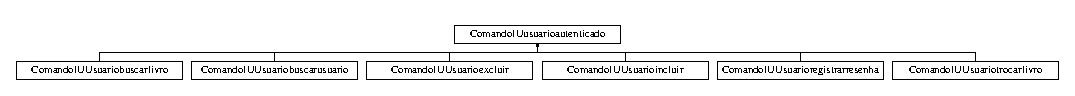
\includegraphics[height=0.844646cm]{classComandoIUusuarioautenticado}
\end{center}
\end{figure}
\subsection*{Public Member Functions}
\begin{DoxyCompactItemize}
\item 
\mbox{\Hypertarget{classComandoIUusuarioautenticado_ac11a39764a6d618e6cc6d870e6209b14}\label{classComandoIUusuarioautenticado_ac11a39764a6d618e6cc6d870e6209b14}} 
virtual void {\bfseries comandosusuarioautenticado} (\hyperlink{classILNComandosusuarioautenticado}{I\+L\+N\+Comandosusuarioautenticado} $\ast$)=0  throw (runtime\+\_\+error)
\end{DoxyCompactItemize}


\subsection{Detailed Description}
Classe de execução dos comandos de um usuário autenticado. 

The documentation for this class was generated from the following files\+:\begin{DoxyCompactItemize}
\item 
comandos.\+h\item 
comandos.\+cpp\end{DoxyCompactItemize}

\hypertarget{classComandoIUUsuariobuscarlivro}{}\section{Comando\+I\+U\+Usuariobuscarlivro Class Reference}
\label{classComandoIUUsuariobuscarlivro}\index{Comando\+I\+U\+Usuariobuscarlivro@{Comando\+I\+U\+Usuariobuscarlivro}}


Classe do comando de busca de livros um usuário autenticado.  




{\ttfamily \#include $<$comandos.\+h$>$}

Inheritance diagram for Comando\+I\+U\+Usuariobuscarlivro\+:\begin{figure}[H]
\begin{center}
\leavevmode
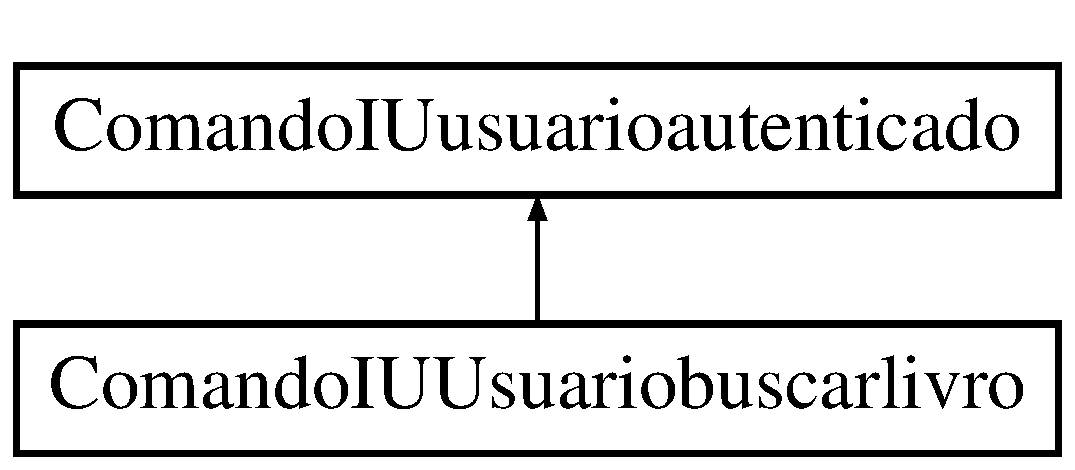
\includegraphics[height=2.000000cm]{classComandoIUUsuariobuscarlivro}
\end{center}
\end{figure}
\subsection*{Public Member Functions}
\begin{DoxyCompactItemize}
\item 
void \hyperlink{classComandoIUUsuariobuscarlivro_a366a108bac44b73daa0777557811e514}{comandosusuarioautenticado} (\hyperlink{classILNComandosusuarioautenticado}{I\+L\+N\+Comandosusuarioautenticado} $\ast$)  throw (runtime\+\_\+error)
\end{DoxyCompactItemize}


\subsection{Detailed Description}
Classe do comando de busca de livros um usuário autenticado. 

\subsection{Member Function Documentation}
\mbox{\Hypertarget{classComandoIUUsuariobuscarlivro_a366a108bac44b73daa0777557811e514}\label{classComandoIUUsuariobuscarlivro_a366a108bac44b73daa0777557811e514}} 
\index{Comando\+I\+U\+Usuariobuscarlivro@{Comando\+I\+U\+Usuariobuscarlivro}!comandosusuarioautenticado@{comandosusuarioautenticado}}
\index{comandosusuarioautenticado@{comandosusuarioautenticado}!Comando\+I\+U\+Usuariobuscarlivro@{Comando\+I\+U\+Usuariobuscarlivro}}
\subsubsection{\texorpdfstring{comandosusuarioautenticado()}{comandosusuarioautenticado()}}
{\footnotesize\ttfamily void Comando\+I\+U\+Usuariobuscarlivro\+::comandosusuarioautenticado (\begin{DoxyParamCaption}\item[{\hyperlink{classILNComandosusuarioautenticado}{I\+L\+N\+Comandosusuarioautenticado} $\ast$}]{cntr\+L\+N\+Comandosusuarioautenticado }\end{DoxyParamCaption}) throw  runtime\+\_\+error) \hspace{0.3cm}{\ttfamily [virtual]}}

Método de comando de busca de livros da controladora 

Implements \hyperlink{classComandoIUusuarioautenticado}{Comando\+I\+Uusuarioautenticado}.



The documentation for this class was generated from the following files\+:\begin{DoxyCompactItemize}
\item 
comandos.\+h\item 
comandos.\+cpp\end{DoxyCompactItemize}

\hypertarget{classComandoIUUsuariobuscarusuario}{}\section{Comando\+I\+U\+Usuariobuscarusuario Class Reference}
\label{classComandoIUUsuariobuscarusuario}\index{Comando\+I\+U\+Usuariobuscarusuario@{Comando\+I\+U\+Usuariobuscarusuario}}


Classe do comando de busca de usuarios de um usuário autenticado.  




{\ttfamily \#include $<$comandos.\+h$>$}

Inheritance diagram for Comando\+I\+U\+Usuariobuscarusuario\+:\begin{figure}[H]
\begin{center}
\leavevmode
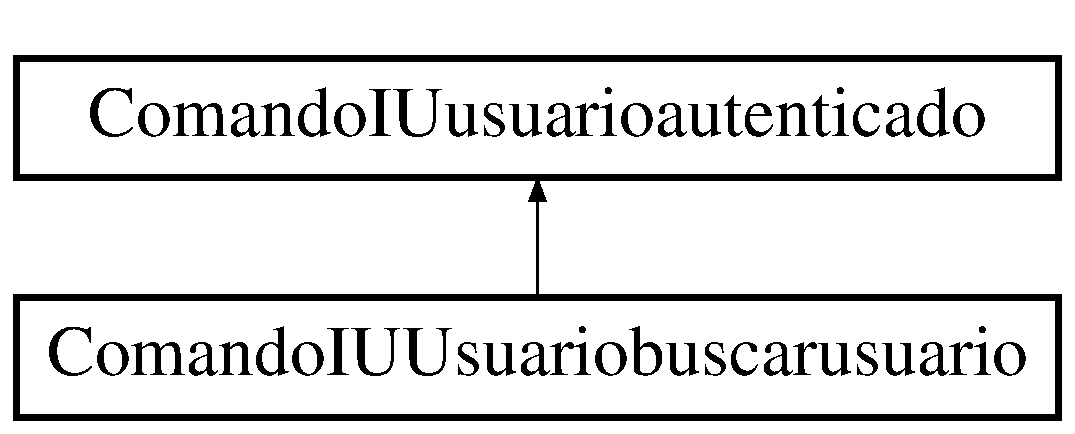
\includegraphics[height=2.000000cm]{classComandoIUUsuariobuscarusuario}
\end{center}
\end{figure}
\subsection*{Public Member Functions}
\begin{DoxyCompactItemize}
\item 
void \hyperlink{classComandoIUUsuariobuscarusuario_af1bcc7671932c7394b3c1b459e64b574}{comandosusuarioautenticado} (\hyperlink{classILNComandosusuarioautenticado}{I\+L\+N\+Comandosusuarioautenticado} $\ast$)  throw (runtime\+\_\+error)
\end{DoxyCompactItemize}


\subsection{Detailed Description}
Classe do comando de busca de usuarios de um usuário autenticado. 

\subsection{Member Function Documentation}
\mbox{\Hypertarget{classComandoIUUsuariobuscarusuario_af1bcc7671932c7394b3c1b459e64b574}\label{classComandoIUUsuariobuscarusuario_af1bcc7671932c7394b3c1b459e64b574}} 
\index{Comando\+I\+U\+Usuariobuscarusuario@{Comando\+I\+U\+Usuariobuscarusuario}!comandosusuarioautenticado@{comandosusuarioautenticado}}
\index{comandosusuarioautenticado@{comandosusuarioautenticado}!Comando\+I\+U\+Usuariobuscarusuario@{Comando\+I\+U\+Usuariobuscarusuario}}
\subsubsection{\texorpdfstring{comandosusuarioautenticado()}{comandosusuarioautenticado()}}
{\footnotesize\ttfamily void Comando\+I\+U\+Usuariobuscarusuario\+::comandosusuarioautenticado (\begin{DoxyParamCaption}\item[{\hyperlink{classILNComandosusuarioautenticado}{I\+L\+N\+Comandosusuarioautenticado} $\ast$}]{cntr\+L\+N\+Comandosusuarioautenticado }\end{DoxyParamCaption}) throw  runtime\+\_\+error) \hspace{0.3cm}{\ttfamily [virtual]}}

Método de comando de busca de usuario da controladora 

Implements \hyperlink{classComandoIUusuarioautenticado}{Comando\+I\+Uusuarioautenticado}.



The documentation for this class was generated from the following files\+:\begin{DoxyCompactItemize}
\item 
comandos.\+h\item 
comandos.\+cpp\end{DoxyCompactItemize}

\hypertarget{classComandoIUUsuarioexcluir}{}\section{Comando\+I\+U\+Usuarioexcluir Class Reference}
\label{classComandoIUUsuarioexcluir}\index{Comando\+I\+U\+Usuarioexcluir@{Comando\+I\+U\+Usuarioexcluir}}


Classe do comando de exclusão de um usuário autenticado.  




{\ttfamily \#include $<$comandos.\+h$>$}

Inheritance diagram for Comando\+I\+U\+Usuarioexcluir\+:\begin{figure}[H]
\begin{center}
\leavevmode
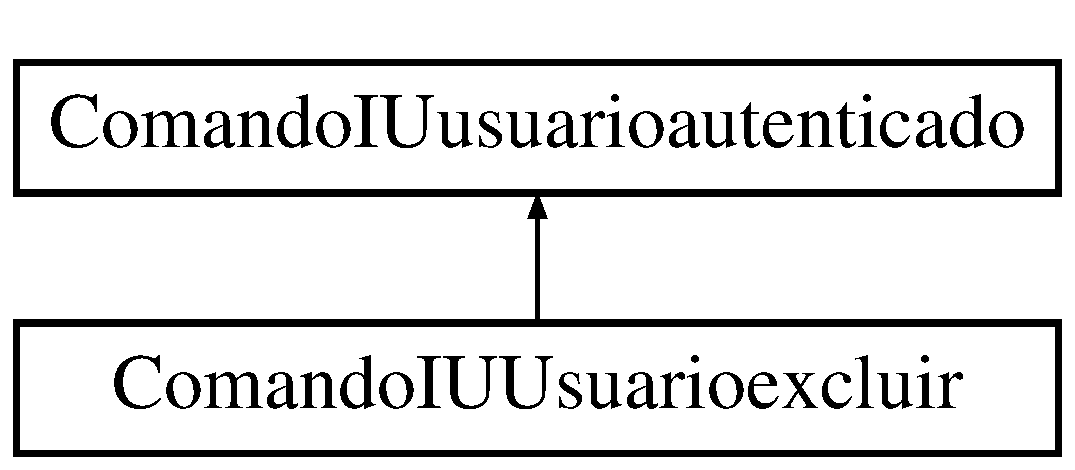
\includegraphics[height=2.000000cm]{classComandoIUUsuarioexcluir}
\end{center}
\end{figure}
\subsection*{Public Member Functions}
\begin{DoxyCompactItemize}
\item 
void \hyperlink{classComandoIUUsuarioexcluir_a891b23e41ec18031eb81f978796a7163}{comandosusuarioautenticado} (\hyperlink{classILNComandosusuarioautenticado}{I\+L\+N\+Comandosusuarioautenticado} $\ast$)  throw (runtime\+\_\+error)
\end{DoxyCompactItemize}


\subsection{Detailed Description}
Classe do comando de exclusão de um usuário autenticado. 

\subsection{Member Function Documentation}
\mbox{\Hypertarget{classComandoIUUsuarioexcluir_a891b23e41ec18031eb81f978796a7163}\label{classComandoIUUsuarioexcluir_a891b23e41ec18031eb81f978796a7163}} 
\index{Comando\+I\+U\+Usuarioexcluir@{Comando\+I\+U\+Usuarioexcluir}!comandosusuarioautenticado@{comandosusuarioautenticado}}
\index{comandosusuarioautenticado@{comandosusuarioautenticado}!Comando\+I\+U\+Usuarioexcluir@{Comando\+I\+U\+Usuarioexcluir}}
\subsubsection{\texorpdfstring{comandosusuarioautenticado()}{comandosusuarioautenticado()}}
{\footnotesize\ttfamily void Comando\+I\+U\+Usuarioexcluir\+::comandosusuarioautenticado (\begin{DoxyParamCaption}\item[{\hyperlink{classILNComandosusuarioautenticado}{I\+L\+N\+Comandosusuarioautenticado} $\ast$}]{cntr\+L\+N\+Comandosusuarioautenticado }\end{DoxyParamCaption}) throw  runtime\+\_\+error) \hspace{0.3cm}{\ttfamily [virtual]}}

Método de comando de exclusao da controladora 

Implements \hyperlink{classComandoIUusuarioautenticado}{Comando\+I\+Uusuarioautenticado}.



The documentation for this class was generated from the following files\+:\begin{DoxyCompactItemize}
\item 
comandos.\+h\item 
comandos.\+cpp\end{DoxyCompactItemize}

\hypertarget{classComandoIUUsuarioincluir}{}\section{Comando\+I\+U\+Usuarioincluir Class Reference}
\label{classComandoIUUsuarioincluir}\index{Comando\+I\+U\+Usuarioincluir@{Comando\+I\+U\+Usuarioincluir}}


Classe do comando de inclusão de um usuário autenticado.  




{\ttfamily \#include $<$comandos.\+h$>$}

Inheritance diagram for Comando\+I\+U\+Usuarioincluir\+:\begin{figure}[H]
\begin{center}
\leavevmode
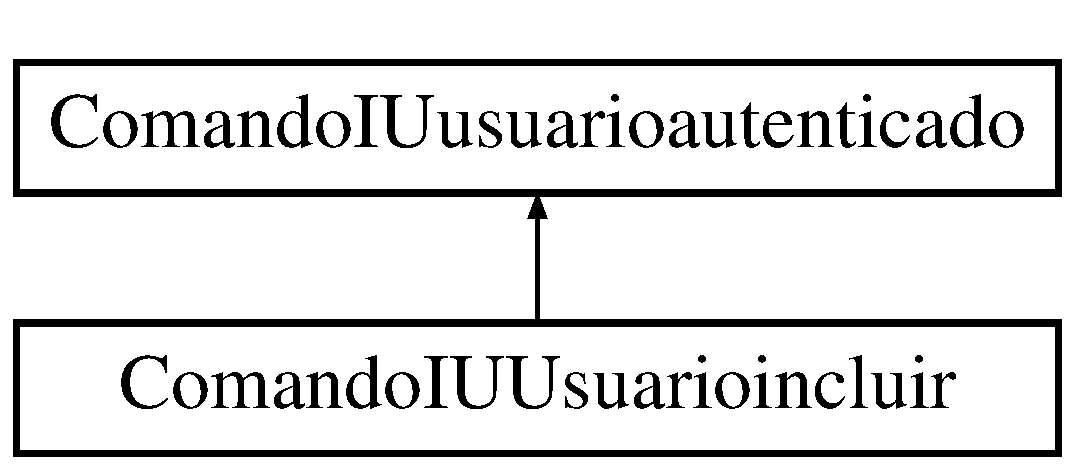
\includegraphics[height=2.000000cm]{classComandoIUUsuarioincluir}
\end{center}
\end{figure}
\subsection*{Public Member Functions}
\begin{DoxyCompactItemize}
\item 
void \hyperlink{classComandoIUUsuarioincluir_a10d61b3ff5e7a675699132662cb82887}{comandosusuarioautenticado} (\hyperlink{classILNComandosusuarioautenticado}{I\+L\+N\+Comandosusuarioautenticado} $\ast$)  throw (runtime\+\_\+error)
\end{DoxyCompactItemize}


\subsection{Detailed Description}
Classe do comando de inclusão de um usuário autenticado. 

\subsection{Member Function Documentation}
\mbox{\Hypertarget{classComandoIUUsuarioincluir_a10d61b3ff5e7a675699132662cb82887}\label{classComandoIUUsuarioincluir_a10d61b3ff5e7a675699132662cb82887}} 
\index{Comando\+I\+U\+Usuarioincluir@{Comando\+I\+U\+Usuarioincluir}!comandosusuarioautenticado@{comandosusuarioautenticado}}
\index{comandosusuarioautenticado@{comandosusuarioautenticado}!Comando\+I\+U\+Usuarioincluir@{Comando\+I\+U\+Usuarioincluir}}
\subsubsection{\texorpdfstring{comandosusuarioautenticado()}{comandosusuarioautenticado()}}
{\footnotesize\ttfamily void Comando\+I\+U\+Usuarioincluir\+::comandosusuarioautenticado (\begin{DoxyParamCaption}\item[{\hyperlink{classILNComandosusuarioautenticado}{I\+L\+N\+Comandosusuarioautenticado} $\ast$}]{cntr\+L\+N\+Comandosusuarioautenticado }\end{DoxyParamCaption}) throw  runtime\+\_\+error) \hspace{0.3cm}{\ttfamily [virtual]}}

Método de comando de inclusao da controladora 

Implements \hyperlink{classComandoIUusuarioautenticado}{Comando\+I\+Uusuarioautenticado}.



The documentation for this class was generated from the following files\+:\begin{DoxyCompactItemize}
\item 
comandos.\+h\item 
comandos.\+cpp\end{DoxyCompactItemize}

\hypertarget{classComandoIUUsuarioregistrarresenha}{}\section{Comando\+I\+U\+Usuarioregistrarresenha Class Reference}
\label{classComandoIUUsuarioregistrarresenha}\index{Comando\+I\+U\+Usuarioregistrarresenha@{Comando\+I\+U\+Usuarioregistrarresenha}}


Classe do comando de registro de resenha de um usuário autenticado.  




{\ttfamily \#include $<$comandos.\+h$>$}

Inheritance diagram for Comando\+I\+U\+Usuarioregistrarresenha\+:\begin{figure}[H]
\begin{center}
\leavevmode
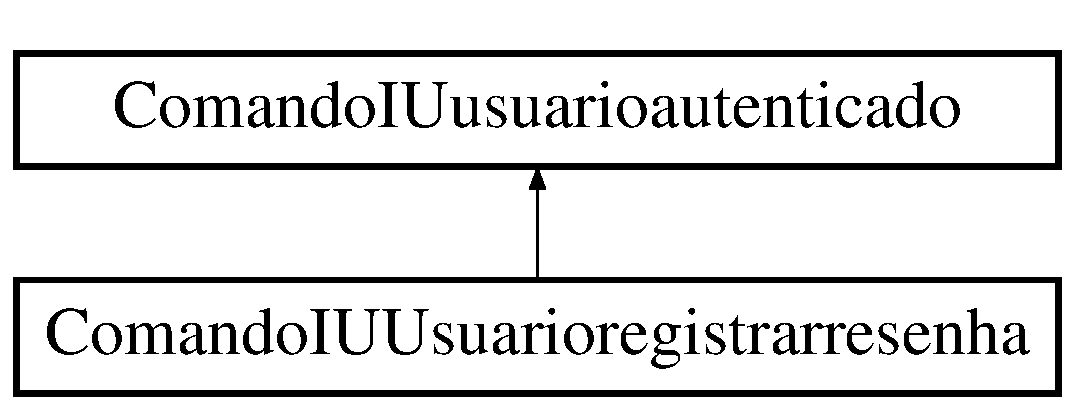
\includegraphics[height=2.000000cm]{classComandoIUUsuarioregistrarresenha}
\end{center}
\end{figure}
\subsection*{Public Member Functions}
\begin{DoxyCompactItemize}
\item 
void \hyperlink{classComandoIUUsuarioregistrarresenha_a606646855da85764201ca85d37884a71}{comandosusuarioautenticado} (\hyperlink{classILNComandosusuarioautenticado}{I\+L\+N\+Comandosusuarioautenticado} $\ast$)  throw (runtime\+\_\+error)
\end{DoxyCompactItemize}


\subsection{Detailed Description}
Classe do comando de registro de resenha de um usuário autenticado. 

\subsection{Member Function Documentation}
\mbox{\Hypertarget{classComandoIUUsuarioregistrarresenha_a606646855da85764201ca85d37884a71}\label{classComandoIUUsuarioregistrarresenha_a606646855da85764201ca85d37884a71}} 
\index{Comando\+I\+U\+Usuarioregistrarresenha@{Comando\+I\+U\+Usuarioregistrarresenha}!comandosusuarioautenticado@{comandosusuarioautenticado}}
\index{comandosusuarioautenticado@{comandosusuarioautenticado}!Comando\+I\+U\+Usuarioregistrarresenha@{Comando\+I\+U\+Usuarioregistrarresenha}}
\subsubsection{\texorpdfstring{comandosusuarioautenticado()}{comandosusuarioautenticado()}}
{\footnotesize\ttfamily void Comando\+I\+U\+Usuarioregistrarresenha\+::comandosusuarioautenticado (\begin{DoxyParamCaption}\item[{\hyperlink{classILNComandosusuarioautenticado}{I\+L\+N\+Comandosusuarioautenticado} $\ast$}]{cntr\+L\+N\+Comandosusuarioautenticado }\end{DoxyParamCaption}) throw  runtime\+\_\+error) \hspace{0.3cm}{\ttfamily [virtual]}}

Método de comando de registro de resenhas da controladora 

Implements \hyperlink{classComandoIUusuarioautenticado}{Comando\+I\+Uusuarioautenticado}.



The documentation for this class was generated from the following files\+:\begin{DoxyCompactItemize}
\item 
comandos.\+h\item 
comandos.\+cpp\end{DoxyCompactItemize}

\hypertarget{classComandoIUUsuariotrocarlivro}{}\section{Comando\+I\+U\+Usuariotrocarlivro Class Reference}
\label{classComandoIUUsuariotrocarlivro}\index{Comando\+I\+U\+Usuariotrocarlivro@{Comando\+I\+U\+Usuariotrocarlivro}}


Classe do comando de troca de livros de um usuário autenticado.  




{\ttfamily \#include $<$comandos.\+h$>$}

Inheritance diagram for Comando\+I\+U\+Usuariotrocarlivro\+:\begin{figure}[H]
\begin{center}
\leavevmode
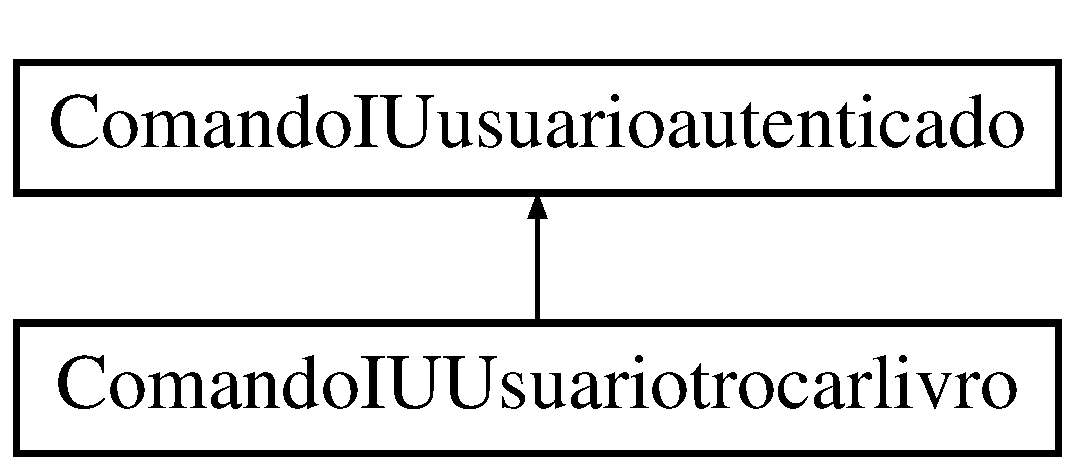
\includegraphics[height=2.000000cm]{classComandoIUUsuariotrocarlivro}
\end{center}
\end{figure}
\subsection*{Public Member Functions}
\begin{DoxyCompactItemize}
\item 
void \hyperlink{classComandoIUUsuariotrocarlivro_acc17db322d213c4bb8780e7896a466d7}{comandosusuarioautenticado} (\hyperlink{classILNComandosusuarioautenticado}{I\+L\+N\+Comandosusuarioautenticado} $\ast$)  throw (runtime\+\_\+error)
\end{DoxyCompactItemize}


\subsection{Detailed Description}
Classe do comando de troca de livros de um usuário autenticado. 

\subsection{Member Function Documentation}
\mbox{\Hypertarget{classComandoIUUsuariotrocarlivro_acc17db322d213c4bb8780e7896a466d7}\label{classComandoIUUsuariotrocarlivro_acc17db322d213c4bb8780e7896a466d7}} 
\index{Comando\+I\+U\+Usuariotrocarlivro@{Comando\+I\+U\+Usuariotrocarlivro}!comandosusuarioautenticado@{comandosusuarioautenticado}}
\index{comandosusuarioautenticado@{comandosusuarioautenticado}!Comando\+I\+U\+Usuariotrocarlivro@{Comando\+I\+U\+Usuariotrocarlivro}}
\subsubsection{\texorpdfstring{comandosusuarioautenticado()}{comandosusuarioautenticado()}}
{\footnotesize\ttfamily void Comando\+I\+U\+Usuariotrocarlivro\+::comandosusuarioautenticado (\begin{DoxyParamCaption}\item[{\hyperlink{classILNComandosusuarioautenticado}{I\+L\+N\+Comandosusuarioautenticado} $\ast$}]{cntr\+L\+N\+Comandosusuarioautenticado }\end{DoxyParamCaption}) throw  runtime\+\_\+error) \hspace{0.3cm}{\ttfamily [virtual]}}

Método de comando de troca de livros da controladora 

Implements \hyperlink{classComandoIUusuarioautenticado}{Comando\+I\+Uusuarioautenticado}.



The documentation for this class was generated from the following files\+:\begin{DoxyCompactItemize}
\item 
comandos.\+h\item 
comandos.\+cpp\end{DoxyCompactItemize}

\hypertarget{classCTRLAutenticacao}{}\section{C\+T\+R\+L\+Autenticacao Class Reference}
\label{classCTRLAutenticacao}\index{C\+T\+R\+L\+Autenticacao@{C\+T\+R\+L\+Autenticacao}}


Classe controladora da autenticação.  




{\ttfamily \#include $<$controladoras.\+h$>$}

Inheritance diagram for C\+T\+R\+L\+Autenticacao\+:\begin{figure}[H]
\begin{center}
\leavevmode
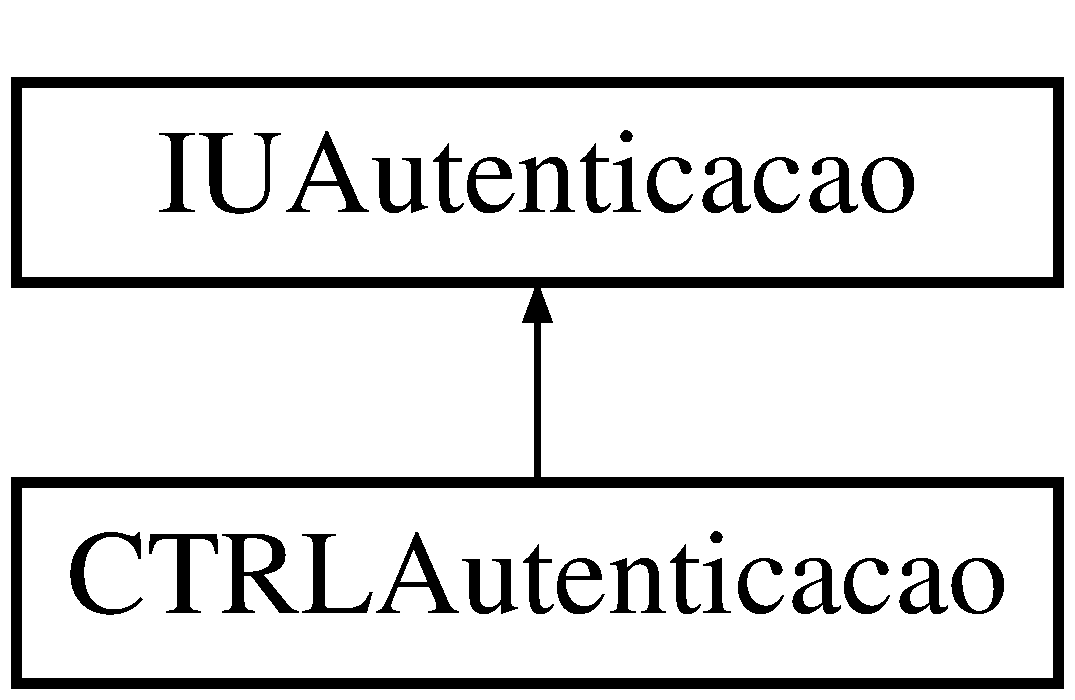
\includegraphics[height=2.000000cm]{classCTRLAutenticacao}
\end{center}
\end{figure}
\subsection*{Public Member Functions}
\begin{DoxyCompactItemize}
\item 
\hyperlink{classResultado}{Resultado} \hyperlink{classCTRLAutenticacao_a9758636458f90f8054637e70a94f1825}{autenticar} ()  throw (runtime\+\_\+error)
\item 
void \hyperlink{classCTRLAutenticacao_aa81983ebd30b5ec21e49670034ebd2b9}{set\+Cntr\+L\+N\+Autenticacao} (\hyperlink{classILNAutenticacao}{I\+L\+N\+Autenticacao} $\ast$)
\end{DoxyCompactItemize}


\subsection{Detailed Description}
Classe controladora da autenticação. 

\subsection{Member Function Documentation}
\mbox{\Hypertarget{classCTRLAutenticacao_a9758636458f90f8054637e70a94f1825}\label{classCTRLAutenticacao_a9758636458f90f8054637e70a94f1825}} 
\index{C\+T\+R\+L\+Autenticacao@{C\+T\+R\+L\+Autenticacao}!autenticar@{autenticar}}
\index{autenticar@{autenticar}!C\+T\+R\+L\+Autenticacao@{C\+T\+R\+L\+Autenticacao}}
\subsubsection{\texorpdfstring{autenticar()}{autenticar()}}
{\footnotesize\ttfamily \hyperlink{classResultado}{Resultado} C\+T\+R\+L\+Autenticacao\+::autenticar (\begin{DoxyParamCaption}{ }\end{DoxyParamCaption}) throw  runtime\+\_\+error) \hspace{0.3cm}{\ttfamily [virtual]}}

Método de autenticação da controladora 

Implements \hyperlink{classIUAutenticacao}{I\+U\+Autenticacao}.

\mbox{\Hypertarget{classCTRLAutenticacao_aa81983ebd30b5ec21e49670034ebd2b9}\label{classCTRLAutenticacao_aa81983ebd30b5ec21e49670034ebd2b9}} 
\index{C\+T\+R\+L\+Autenticacao@{C\+T\+R\+L\+Autenticacao}!set\+Cntr\+L\+N\+Autenticacao@{set\+Cntr\+L\+N\+Autenticacao}}
\index{set\+Cntr\+L\+N\+Autenticacao@{set\+Cntr\+L\+N\+Autenticacao}!C\+T\+R\+L\+Autenticacao@{C\+T\+R\+L\+Autenticacao}}
\subsubsection{\texorpdfstring{set\+Cntr\+L\+N\+Autenticacao()}{setCntrLNAutenticacao()}}
{\footnotesize\ttfamily void C\+T\+R\+L\+Autenticacao\+::set\+Cntr\+L\+N\+Autenticacao (\begin{DoxyParamCaption}\item[{\hyperlink{classILNAutenticacao}{I\+L\+N\+Autenticacao} $\ast$}]{L\+N\+Autenticacao }\end{DoxyParamCaption})\hspace{0.3cm}{\ttfamily [inline]}, {\ttfamily [virtual]}}

Método responsável por fazer a ligação entre controladora de autenticação e lógica de negócio 

Implements \hyperlink{classIUAutenticacao}{I\+U\+Autenticacao}.



The documentation for this class was generated from the following files\+:\begin{DoxyCompactItemize}
\item 
controladoras.\+h\item 
controladoras.\+cpp\end{DoxyCompactItemize}

\hypertarget{classCTRLBuscarlivro}{}\section{C\+T\+R\+L\+Buscarlivro Class Reference}
\label{classCTRLBuscarlivro}\index{C\+T\+R\+L\+Buscarlivro@{C\+T\+R\+L\+Buscarlivro}}


Classe controladora da busca de livros.  




{\ttfamily \#include $<$controladoras.\+h$>$}

Inheritance diagram for C\+T\+R\+L\+Buscarlivro\+:\begin{figure}[H]
\begin{center}
\leavevmode
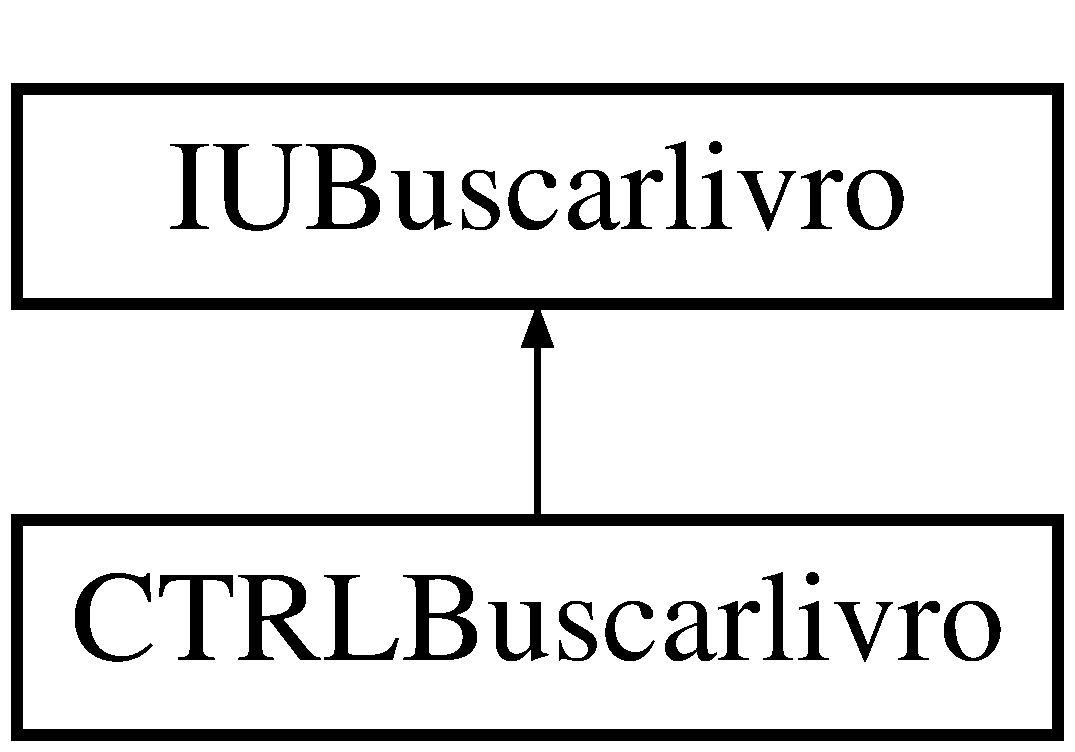
\includegraphics[height=2.000000cm]{classCTRLBuscarlivro}
\end{center}
\end{figure}
\subsection*{Public Member Functions}
\begin{DoxyCompactItemize}
\item 
\hyperlink{classResultado}{Resultado} \hyperlink{classCTRLBuscarlivro_a220f5a7d88a1316eb04a37cacc20c542}{buscarlivro} (\hyperlink{classLivro}{Livro} $\ast$$\ast$)  throw (runtime\+\_\+error)
\item 
\mbox{\Hypertarget{classCTRLBuscarlivro_a9ba558c715f6af58b8694b8fbd8cde49}\label{classCTRLBuscarlivro_a9ba558c715f6af58b8694b8fbd8cde49}} 
void {\bfseries set\+Container} (\hyperlink{classContainerLivro}{Container\+Livro} $\ast$)
\end{DoxyCompactItemize}


\subsection{Detailed Description}
Classe controladora da busca de livros. 

\subsection{Member Function Documentation}
\mbox{\Hypertarget{classCTRLBuscarlivro_a220f5a7d88a1316eb04a37cacc20c542}\label{classCTRLBuscarlivro_a220f5a7d88a1316eb04a37cacc20c542}} 
\index{C\+T\+R\+L\+Buscarlivro@{C\+T\+R\+L\+Buscarlivro}!buscarlivro@{buscarlivro}}
\index{buscarlivro@{buscarlivro}!C\+T\+R\+L\+Buscarlivro@{C\+T\+R\+L\+Buscarlivro}}
\subsubsection{\texorpdfstring{buscarlivro()}{buscarlivro()}}
{\footnotesize\ttfamily \hyperlink{classResultado}{Resultado} C\+T\+R\+L\+Buscarlivro\+::buscarlivro (\begin{DoxyParamCaption}\item[{\hyperlink{classLivro}{Livro} $\ast$$\ast$}]{livro }\end{DoxyParamCaption}) throw  runtime\+\_\+error) \hspace{0.3cm}{\ttfamily [virtual]}}

Método de busca de livros da controladora 

Implements \hyperlink{classIUBuscarlivro}{I\+U\+Buscarlivro}.



The documentation for this class was generated from the following files\+:\begin{DoxyCompactItemize}
\item 
controladoras.\+h\item 
controladoras.\+cpp\end{DoxyCompactItemize}

\hypertarget{classCTRLBuscarusuario}{}\section{C\+T\+R\+L\+Buscarusuario Class Reference}
\label{classCTRLBuscarusuario}\index{C\+T\+R\+L\+Buscarusuario@{C\+T\+R\+L\+Buscarusuario}}


Classe controladora da busca de usuários.  




{\ttfamily \#include $<$controladoras.\+h$>$}

Inheritance diagram for C\+T\+R\+L\+Buscarusuario\+:\begin{figure}[H]
\begin{center}
\leavevmode
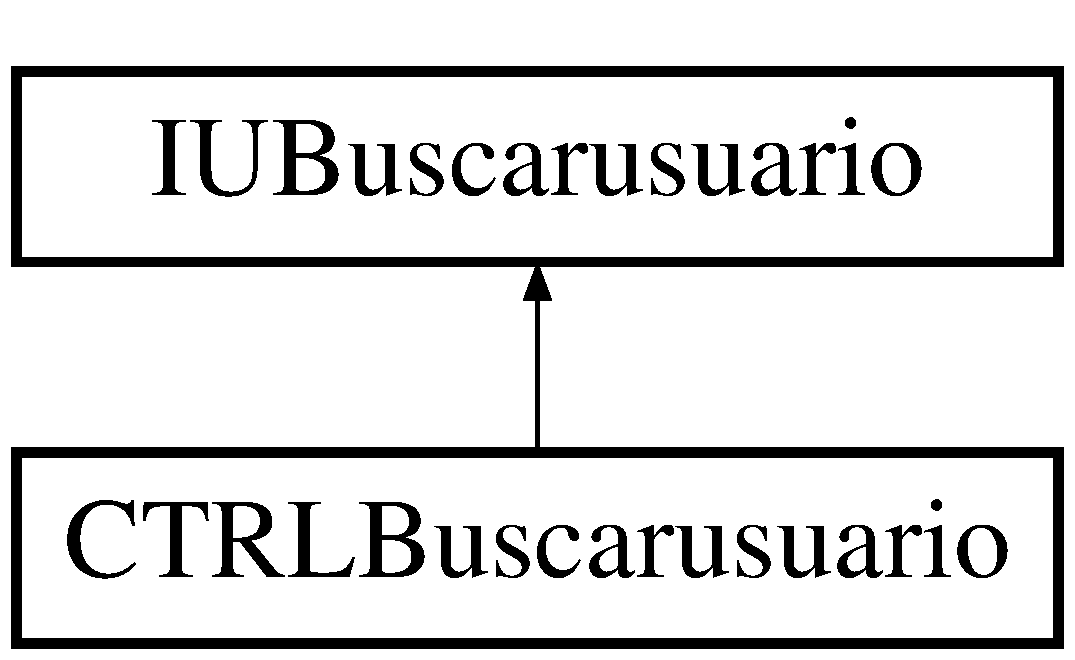
\includegraphics[height=2.000000cm]{classCTRLBuscarusuario}
\end{center}
\end{figure}
\subsection*{Public Member Functions}
\begin{DoxyCompactItemize}
\item 
\hyperlink{classResultado}{Resultado} \hyperlink{classCTRLBuscarusuario_a4c73f22cb6b0083a99a21e3abe45cc5a}{buscarusuario} ()  throw (runtime\+\_\+error)
\item 
void \hyperlink{classCTRLBuscarusuario_afb7a2a586b958579f7a777b3d93da661}{set\+Cntr\+L\+N\+Buscarusuario} (\hyperlink{classILNBuscarusuario}{I\+L\+N\+Buscarusuario} $\ast$)
\end{DoxyCompactItemize}


\subsection{Detailed Description}
Classe controladora da busca de usuários. 

\subsection{Member Function Documentation}
\mbox{\Hypertarget{classCTRLBuscarusuario_a4c73f22cb6b0083a99a21e3abe45cc5a}\label{classCTRLBuscarusuario_a4c73f22cb6b0083a99a21e3abe45cc5a}} 
\index{C\+T\+R\+L\+Buscarusuario@{C\+T\+R\+L\+Buscarusuario}!buscarusuario@{buscarusuario}}
\index{buscarusuario@{buscarusuario}!C\+T\+R\+L\+Buscarusuario@{C\+T\+R\+L\+Buscarusuario}}
\subsubsection{\texorpdfstring{buscarusuario()}{buscarusuario()}}
{\footnotesize\ttfamily \hyperlink{classResultado}{Resultado} C\+T\+R\+L\+Buscarusuario\+::buscarusuario (\begin{DoxyParamCaption}{ }\end{DoxyParamCaption}) throw  runtime\+\_\+error) \hspace{0.3cm}{\ttfamily [virtual]}}

Método de busca de usuários da controladora 

Implements \hyperlink{classIUBuscarusuario}{I\+U\+Buscarusuario}.

\mbox{\Hypertarget{classCTRLBuscarusuario_afb7a2a586b958579f7a777b3d93da661}\label{classCTRLBuscarusuario_afb7a2a586b958579f7a777b3d93da661}} 
\index{C\+T\+R\+L\+Buscarusuario@{C\+T\+R\+L\+Buscarusuario}!set\+Cntr\+L\+N\+Buscarusuario@{set\+Cntr\+L\+N\+Buscarusuario}}
\index{set\+Cntr\+L\+N\+Buscarusuario@{set\+Cntr\+L\+N\+Buscarusuario}!C\+T\+R\+L\+Buscarusuario@{C\+T\+R\+L\+Buscarusuario}}
\subsubsection{\texorpdfstring{set\+Cntr\+L\+N\+Buscarusuario()}{setCntrLNBuscarusuario()}}
{\footnotesize\ttfamily void C\+T\+R\+L\+Buscarusuario\+::set\+Cntr\+L\+N\+Buscarusuario (\begin{DoxyParamCaption}\item[{\hyperlink{classILNBuscarusuario}{I\+L\+N\+Buscarusuario} $\ast$}]{L\+N\+Buscarusuario }\end{DoxyParamCaption})\hspace{0.3cm}{\ttfamily [inline]}, {\ttfamily [virtual]}}

Método responsável por fazer a ligação entre controladora de busca de usuários e lógica de negócio 

Implements \hyperlink{classIUBuscarusuario}{I\+U\+Buscarusuario}.



The documentation for this class was generated from the following files\+:\begin{DoxyCompactItemize}
\item 
controladoras.\+h\item 
controladoras.\+cpp\end{DoxyCompactItemize}

\hypertarget{classCTRLCadastro}{}\section{C\+T\+R\+L\+Cadastro Class Reference}
\label{classCTRLCadastro}\index{C\+T\+R\+L\+Cadastro@{C\+T\+R\+L\+Cadastro}}


Classe controladora do cadastro de usuário.  




{\ttfamily \#include $<$controladoras.\+h$>$}

Inheritance diagram for C\+T\+R\+L\+Cadastro\+:\begin{figure}[H]
\begin{center}
\leavevmode
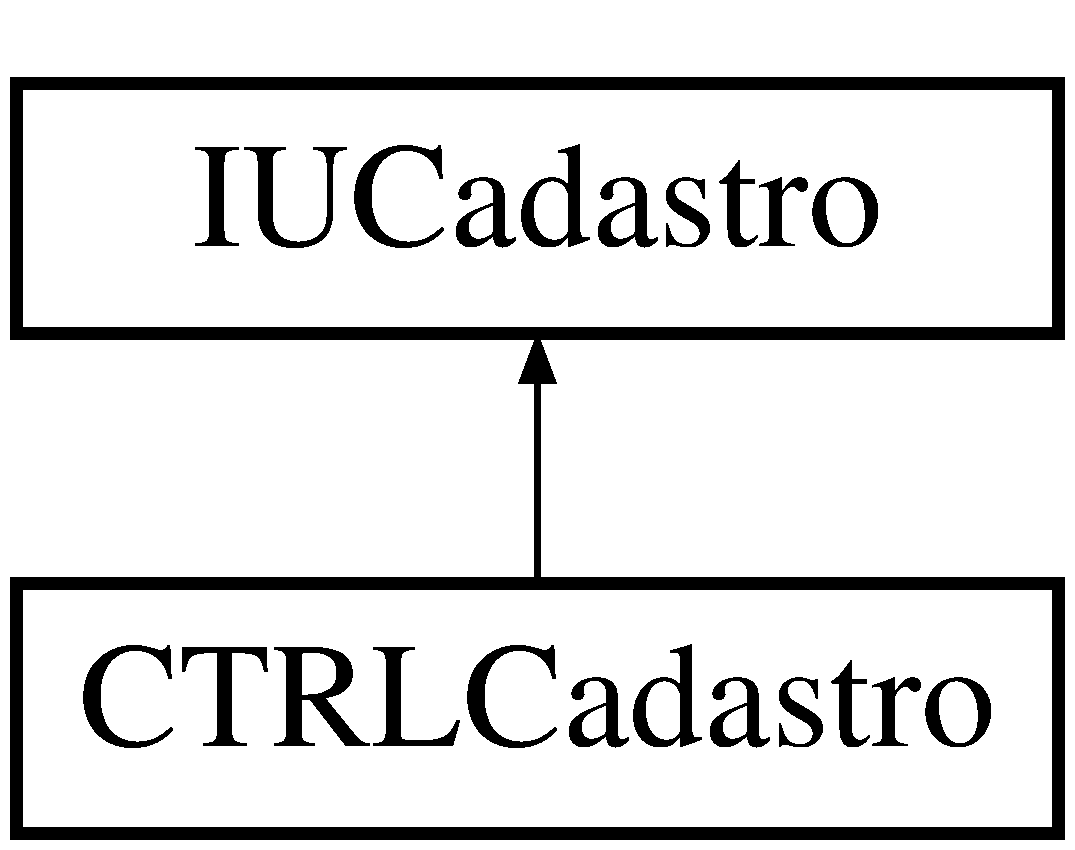
\includegraphics[height=2.000000cm]{classCTRLCadastro}
\end{center}
\end{figure}
\subsection*{Public Member Functions}
\begin{DoxyCompactItemize}
\item 
\hyperlink{classResultado}{Resultado} \hyperlink{classCTRLCadastro_a22e15e47f34bb629a27204be76abf69c}{cadastrar} ()  throw (runtime\+\_\+error)
\item 
void \hyperlink{classCTRLCadastro_aa9324e682be46537c44c2feb33e05991}{set\+Cntr\+L\+N\+Cadastro} (\hyperlink{classILNCadastro}{I\+L\+N\+Cadastro} $\ast$)
\end{DoxyCompactItemize}


\subsection{Detailed Description}
Classe controladora do cadastro de usuário. 

\subsection{Member Function Documentation}
\mbox{\Hypertarget{classCTRLCadastro_a22e15e47f34bb629a27204be76abf69c}\label{classCTRLCadastro_a22e15e47f34bb629a27204be76abf69c}} 
\index{C\+T\+R\+L\+Cadastro@{C\+T\+R\+L\+Cadastro}!cadastrar@{cadastrar}}
\index{cadastrar@{cadastrar}!C\+T\+R\+L\+Cadastro@{C\+T\+R\+L\+Cadastro}}
\subsubsection{\texorpdfstring{cadastrar()}{cadastrar()}}
{\footnotesize\ttfamily \hyperlink{classResultado}{Resultado} C\+T\+R\+L\+Cadastro\+::cadastrar (\begin{DoxyParamCaption}{ }\end{DoxyParamCaption}) throw  runtime\+\_\+error) \hspace{0.3cm}{\ttfamily [virtual]}}

Método de cadastramento de usuário da controladora 

Implements \hyperlink{classIUCadastro}{I\+U\+Cadastro}.

\mbox{\Hypertarget{classCTRLCadastro_aa9324e682be46537c44c2feb33e05991}\label{classCTRLCadastro_aa9324e682be46537c44c2feb33e05991}} 
\index{C\+T\+R\+L\+Cadastro@{C\+T\+R\+L\+Cadastro}!set\+Cntr\+L\+N\+Cadastro@{set\+Cntr\+L\+N\+Cadastro}}
\index{set\+Cntr\+L\+N\+Cadastro@{set\+Cntr\+L\+N\+Cadastro}!C\+T\+R\+L\+Cadastro@{C\+T\+R\+L\+Cadastro}}
\subsubsection{\texorpdfstring{set\+Cntr\+L\+N\+Cadastro()}{setCntrLNCadastro()}}
{\footnotesize\ttfamily void C\+T\+R\+L\+Cadastro\+::set\+Cntr\+L\+N\+Cadastro (\begin{DoxyParamCaption}\item[{\hyperlink{classILNCadastro}{I\+L\+N\+Cadastro} $\ast$}]{L\+N\+Cadastro }\end{DoxyParamCaption})\hspace{0.3cm}{\ttfamily [inline]}, {\ttfamily [virtual]}}

Método responsável por fazer a ligação entre controladora de cadastro de usuário e lógica de negócio 

Implements \hyperlink{classIUCadastro}{I\+U\+Cadastro}.



The documentation for this class was generated from the following files\+:\begin{DoxyCompactItemize}
\item 
controladoras.\+h\item 
controladoras.\+cpp\end{DoxyCompactItemize}

\hypertarget{classCTRLCadastrolivro}{}\section{C\+T\+R\+L\+Cadastrolivro Class Reference}
\label{classCTRLCadastrolivro}\index{C\+T\+R\+L\+Cadastrolivro@{C\+T\+R\+L\+Cadastrolivro}}


Classe controladora do cadastro de livro.  




{\ttfamily \#include $<$controladoras.\+h$>$}

Inheritance diagram for C\+T\+R\+L\+Cadastrolivro\+:\begin{figure}[H]
\begin{center}
\leavevmode
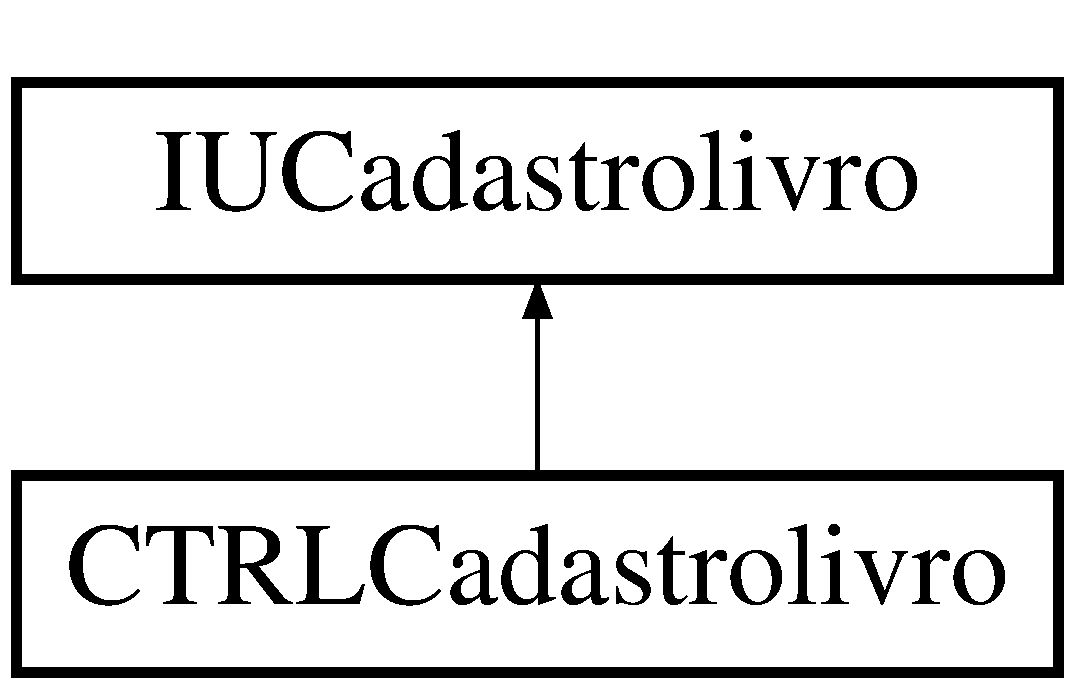
\includegraphics[height=2.000000cm]{classCTRLCadastrolivro}
\end{center}
\end{figure}
\subsection*{Public Member Functions}
\begin{DoxyCompactItemize}
\item 
\hyperlink{classResultado}{Resultado} \hyperlink{classCTRLCadastrolivro_ad932abd7bd49e2a5fbf4ba137c4df381}{cadastrarlivro} ()  throw (runtime\+\_\+error)
\item 
\mbox{\Hypertarget{classCTRLCadastrolivro_aabb75fa8e3d9d4b81df8de87debabe20}\label{classCTRLCadastrolivro_aabb75fa8e3d9d4b81df8de87debabe20}} 
void {\bfseries set\+Container} (\hyperlink{classContainerLivro}{Container\+Livro} $\ast$)
\end{DoxyCompactItemize}


\subsection{Detailed Description}
Classe controladora do cadastro de livro. 

\subsection{Member Function Documentation}
\mbox{\Hypertarget{classCTRLCadastrolivro_ad932abd7bd49e2a5fbf4ba137c4df381}\label{classCTRLCadastrolivro_ad932abd7bd49e2a5fbf4ba137c4df381}} 
\index{C\+T\+R\+L\+Cadastrolivro@{C\+T\+R\+L\+Cadastrolivro}!cadastrarlivro@{cadastrarlivro}}
\index{cadastrarlivro@{cadastrarlivro}!C\+T\+R\+L\+Cadastrolivro@{C\+T\+R\+L\+Cadastrolivro}}
\subsubsection{\texorpdfstring{cadastrarlivro()}{cadastrarlivro()}}
{\footnotesize\ttfamily \hyperlink{classResultado}{Resultado} C\+T\+R\+L\+Cadastrolivro\+::cadastrarlivro (\begin{DoxyParamCaption}{ }\end{DoxyParamCaption}) throw  runtime\+\_\+error) \hspace{0.3cm}{\ttfamily [virtual]}}

Método de cadastramento de livro da controladora 

Implements \hyperlink{classIUCadastrolivro}{I\+U\+Cadastrolivro}.



The documentation for this class was generated from the following files\+:\begin{DoxyCompactItemize}
\item 
controladoras.\+h\item 
controladoras.\+cpp\end{DoxyCompactItemize}

\hypertarget{classCTRLComandosusuarioautenticado}{}\section{C\+T\+R\+L\+Comandosusuarioautenticado Class Reference}
\label{classCTRLComandosusuarioautenticado}\index{C\+T\+R\+L\+Comandosusuarioautenticado@{C\+T\+R\+L\+Comandosusuarioautenticado}}


Classe controladora dos comandos de um usuário autenticado.  




{\ttfamily \#include $<$controladoras.\+h$>$}

Inheritance diagram for C\+T\+R\+L\+Comandosusuarioautenticado\+:\begin{figure}[H]
\begin{center}
\leavevmode
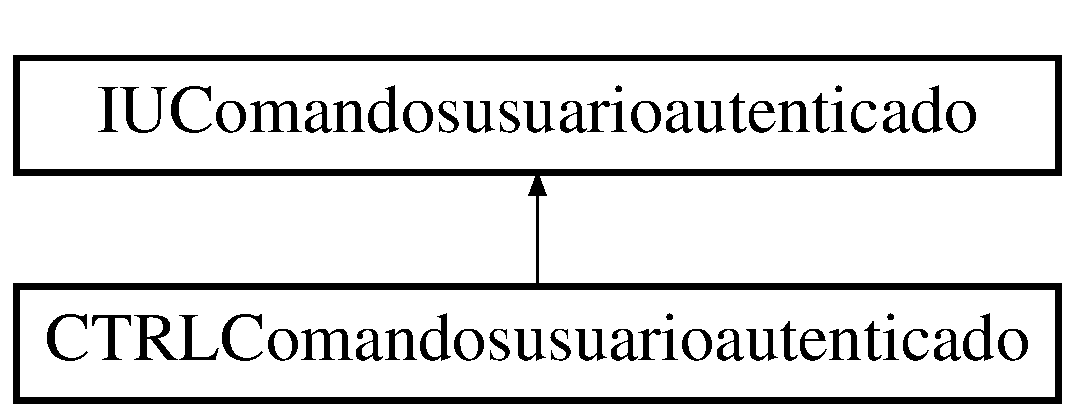
\includegraphics[height=2.000000cm]{classCTRLComandosusuarioautenticado}
\end{center}
\end{figure}
\subsection*{Public Member Functions}
\begin{DoxyCompactItemize}
\item 
void \hyperlink{classCTRLComandosusuarioautenticado_a6c0ee44bfadcf9854fca6fcf4e3379c2}{comandosusuarioautenticado} ()  throw (runtime\+\_\+error)
\item 
void \hyperlink{classCTRLComandosusuarioautenticado_a921e8dec09b5861ea96b737b673ab785}{set\+Cntr\+L\+N\+Comandosusuarioautenticado} (\hyperlink{classILNComandosusuarioautenticado}{I\+L\+N\+Comandosusuarioautenticado} $\ast$)
\end{DoxyCompactItemize}


\subsection{Detailed Description}
Classe controladora dos comandos de um usuário autenticado. 

\subsection{Member Function Documentation}
\mbox{\Hypertarget{classCTRLComandosusuarioautenticado_a6c0ee44bfadcf9854fca6fcf4e3379c2}\label{classCTRLComandosusuarioautenticado_a6c0ee44bfadcf9854fca6fcf4e3379c2}} 
\index{C\+T\+R\+L\+Comandosusuarioautenticado@{C\+T\+R\+L\+Comandosusuarioautenticado}!comandosusuarioautenticado@{comandosusuarioautenticado}}
\index{comandosusuarioautenticado@{comandosusuarioautenticado}!C\+T\+R\+L\+Comandosusuarioautenticado@{C\+T\+R\+L\+Comandosusuarioautenticado}}
\subsubsection{\texorpdfstring{comandosusuarioautenticado()}{comandosusuarioautenticado()}}
{\footnotesize\ttfamily void C\+T\+R\+L\+Comandosusuarioautenticado\+::comandosusuarioautenticado (\begin{DoxyParamCaption}{ }\end{DoxyParamCaption}) throw  runtime\+\_\+error) \hspace{0.3cm}{\ttfamily [virtual]}}

Método de comandos de usuario da controladora 

Implements \hyperlink{classIUComandosusuarioautenticado}{I\+U\+Comandosusuarioautenticado}.

\mbox{\Hypertarget{classCTRLComandosusuarioautenticado_a921e8dec09b5861ea96b737b673ab785}\label{classCTRLComandosusuarioautenticado_a921e8dec09b5861ea96b737b673ab785}} 
\index{C\+T\+R\+L\+Comandosusuarioautenticado@{C\+T\+R\+L\+Comandosusuarioautenticado}!set\+Cntr\+L\+N\+Comandosusuarioautenticado@{set\+Cntr\+L\+N\+Comandosusuarioautenticado}}
\index{set\+Cntr\+L\+N\+Comandosusuarioautenticado@{set\+Cntr\+L\+N\+Comandosusuarioautenticado}!C\+T\+R\+L\+Comandosusuarioautenticado@{C\+T\+R\+L\+Comandosusuarioautenticado}}
\subsubsection{\texorpdfstring{set\+Cntr\+L\+N\+Comandosusuarioautenticado()}{setCntrLNComandosusuarioautenticado()}}
{\footnotesize\ttfamily void C\+T\+R\+L\+Comandosusuarioautenticado\+::set\+Cntr\+L\+N\+Comandosusuarioautenticado (\begin{DoxyParamCaption}\item[{\hyperlink{classILNComandosusuarioautenticado}{I\+L\+N\+Comandosusuarioautenticado} $\ast$}]{cntr\+L\+N\+Comandosusuarioautenticado }\end{DoxyParamCaption})\hspace{0.3cm}{\ttfamily [inline]}, {\ttfamily [virtual]}}

Método responsável por fazer a ligação entre controladora de comandos de um usuário autenticado e lógica de negócio 

Implements \hyperlink{classIUComandosusuarioautenticado}{I\+U\+Comandosusuarioautenticado}.



The documentation for this class was generated from the following files\+:\begin{DoxyCompactItemize}
\item 
controladoras.\+h\item 
controladoras.\+cpp\end{DoxyCompactItemize}

\hypertarget{classCTRLRegistroresenha}{}\section{C\+T\+R\+L\+Registroresenha Class Reference}
\label{classCTRLRegistroresenha}\index{C\+T\+R\+L\+Registroresenha@{C\+T\+R\+L\+Registroresenha}}


Classe controladora do registro de resenhas.  




{\ttfamily \#include $<$controladoras.\+h$>$}

Inheritance diagram for C\+T\+R\+L\+Registroresenha\+:\begin{figure}[H]
\begin{center}
\leavevmode
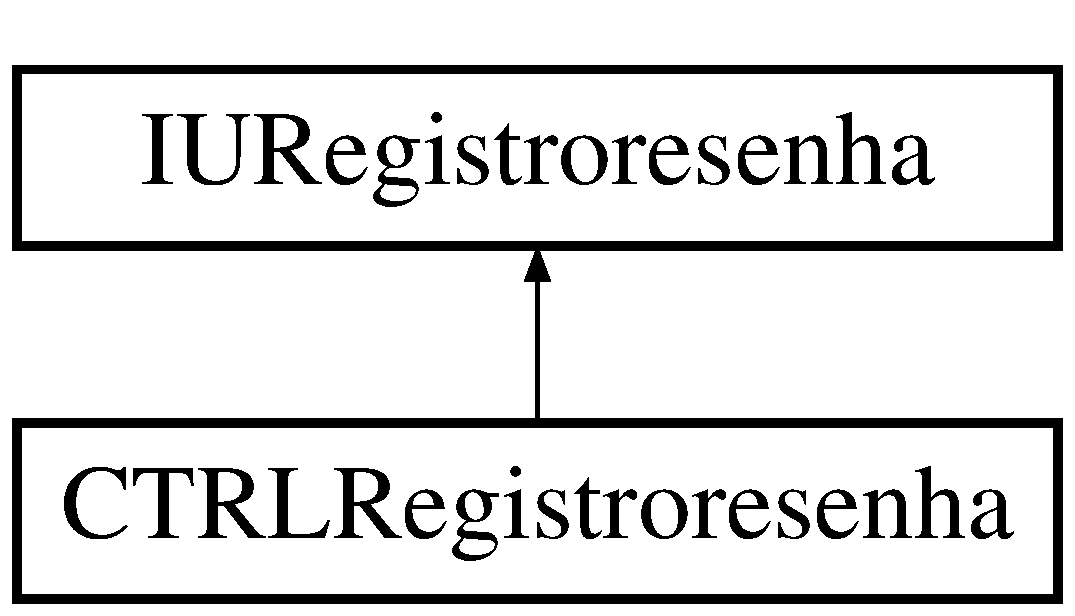
\includegraphics[height=2.000000cm]{classCTRLRegistroresenha}
\end{center}
\end{figure}
\subsection*{Public Member Functions}
\begin{DoxyCompactItemize}
\item 
\hyperlink{classResultado}{Resultado} \hyperlink{classCTRLRegistroresenha_a7ffdc7e6a667bbf5d93c95659944f621}{registrarresenha} (string, string)  throw (runtime\+\_\+error)
\item 
\mbox{\Hypertarget{classCTRLRegistroresenha_ac7ee6ec7da046f2b61b138c996f17d45}\label{classCTRLRegistroresenha_ac7ee6ec7da046f2b61b138c996f17d45}} 
void {\bfseries set\+Container} (\hyperlink{classContainerResenha}{Container\+Resenha} $\ast$)
\end{DoxyCompactItemize}


\subsection{Detailed Description}
Classe controladora do registro de resenhas. 

\subsection{Member Function Documentation}
\mbox{\Hypertarget{classCTRLRegistroresenha_a7ffdc7e6a667bbf5d93c95659944f621}\label{classCTRLRegistroresenha_a7ffdc7e6a667bbf5d93c95659944f621}} 
\index{C\+T\+R\+L\+Registroresenha@{C\+T\+R\+L\+Registroresenha}!registrarresenha@{registrarresenha}}
\index{registrarresenha@{registrarresenha}!C\+T\+R\+L\+Registroresenha@{C\+T\+R\+L\+Registroresenha}}
\subsubsection{\texorpdfstring{registrarresenha()}{registrarresenha()}}
{\footnotesize\ttfamily \hyperlink{classResultado}{Resultado} C\+T\+R\+L\+Registroresenha\+::registrarresenha (\begin{DoxyParamCaption}\item[{string}]{entrada\+\_\+titulo,  }\item[{string}]{entrada\+\_\+autor }\end{DoxyParamCaption}) throw  runtime\+\_\+error) \hspace{0.3cm}{\ttfamily [virtual]}}

Método de registramento de resenha da controladora 

Implements \hyperlink{classIURegistroresenha}{I\+U\+Registroresenha}.



The documentation for this class was generated from the following files\+:\begin{DoxyCompactItemize}
\item 
controladoras.\+h\item 
controladoras.\+cpp\end{DoxyCompactItemize}

\hypertarget{classCTRLTrocarlivro}{}\section{C\+T\+R\+L\+Trocarlivro Class Reference}
\label{classCTRLTrocarlivro}\index{C\+T\+R\+L\+Trocarlivro@{C\+T\+R\+L\+Trocarlivro}}


Classe controladora da troca de livros.  




{\ttfamily \#include $<$controladoras.\+h$>$}

Inheritance diagram for C\+T\+R\+L\+Trocarlivro\+:\begin{figure}[H]
\begin{center}
\leavevmode
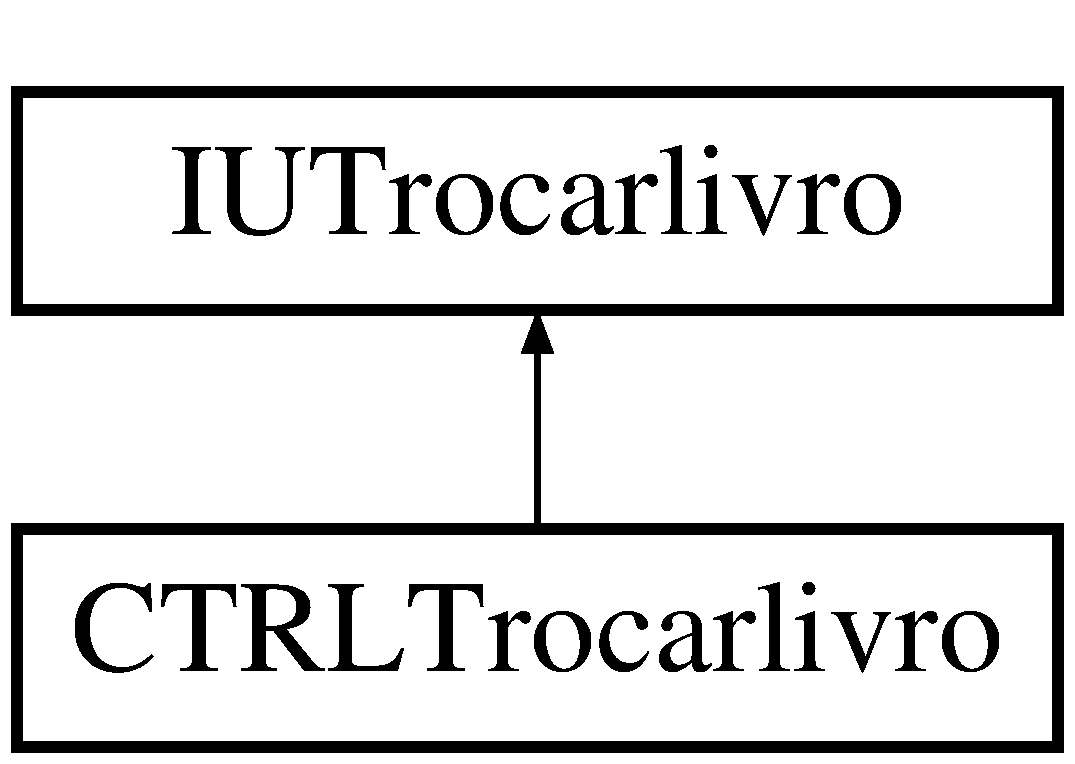
\includegraphics[height=2.000000cm]{classCTRLTrocarlivro}
\end{center}
\end{figure}
\subsection*{Public Member Functions}
\begin{DoxyCompactItemize}
\item 
\hyperlink{classResultado}{Resultado} \hyperlink{classCTRLTrocarlivro_ab0bd103af757427e4272e44dfbe47a49}{trocarlivro} ()  throw (runtime\+\_\+error)
\item 
void \hyperlink{classCTRLTrocarlivro_af157f82ed9d7febfe8f4175d50990e8e}{set\+Cntr\+L\+N\+Trocarlivro} (\hyperlink{classILNTrocarlivro}{I\+L\+N\+Trocarlivro} $\ast$)
\end{DoxyCompactItemize}


\subsection{Detailed Description}
Classe controladora da troca de livros. 

\subsection{Member Function Documentation}
\mbox{\Hypertarget{classCTRLTrocarlivro_af157f82ed9d7febfe8f4175d50990e8e}\label{classCTRLTrocarlivro_af157f82ed9d7febfe8f4175d50990e8e}} 
\index{C\+T\+R\+L\+Trocarlivro@{C\+T\+R\+L\+Trocarlivro}!set\+Cntr\+L\+N\+Trocarlivro@{set\+Cntr\+L\+N\+Trocarlivro}}
\index{set\+Cntr\+L\+N\+Trocarlivro@{set\+Cntr\+L\+N\+Trocarlivro}!C\+T\+R\+L\+Trocarlivro@{C\+T\+R\+L\+Trocarlivro}}
\subsubsection{\texorpdfstring{set\+Cntr\+L\+N\+Trocarlivro()}{setCntrLNTrocarlivro()}}
{\footnotesize\ttfamily void C\+T\+R\+L\+Trocarlivro\+::set\+Cntr\+L\+N\+Trocarlivro (\begin{DoxyParamCaption}\item[{\hyperlink{classILNTrocarlivro}{I\+L\+N\+Trocarlivro} $\ast$}]{L\+N\+Trocarlivro }\end{DoxyParamCaption})\hspace{0.3cm}{\ttfamily [inline]}, {\ttfamily [virtual]}}

Método responsável por fazer a ligação entre controladora de troca de livro e lógica de negócio 

Implements \hyperlink{classIUTrocarlivro}{I\+U\+Trocarlivro}.

\mbox{\Hypertarget{classCTRLTrocarlivro_ab0bd103af757427e4272e44dfbe47a49}\label{classCTRLTrocarlivro_ab0bd103af757427e4272e44dfbe47a49}} 
\index{C\+T\+R\+L\+Trocarlivro@{C\+T\+R\+L\+Trocarlivro}!trocarlivro@{trocarlivro}}
\index{trocarlivro@{trocarlivro}!C\+T\+R\+L\+Trocarlivro@{C\+T\+R\+L\+Trocarlivro}}
\subsubsection{\texorpdfstring{trocarlivro()}{trocarlivro()}}
{\footnotesize\ttfamily \hyperlink{classResultado}{Resultado} C\+T\+R\+L\+Trocarlivro\+::trocarlivro (\begin{DoxyParamCaption}{ }\end{DoxyParamCaption}) throw  runtime\+\_\+error) \hspace{0.3cm}{\ttfamily [virtual]}}

Método de troca de livros da controladora 

Implements \hyperlink{classIUTrocarlivro}{I\+U\+Trocarlivro}.



The documentation for this class was generated from the following files\+:\begin{DoxyCompactItemize}
\item 
controladoras.\+h\item 
controladoras.\+cpp\end{DoxyCompactItemize}

\hypertarget{classData}{}\section{Data Class Reference}
\label{classData}\index{Data@{Data}}
\subsection*{Public Member Functions}
\begin{DoxyCompactItemize}
\item 
\mbox{\Hypertarget{classData_a75a50f88bc966f20826a3959717a5acc}\label{classData_a75a50f88bc966f20826a3959717a5acc}} 
void {\bfseries set\+Data} (string)  throw (invalid\+\_\+argument)
\item 
\mbox{\Hypertarget{classData_a13f25eafdc138d743e99eb4086d765a2}\label{classData_a13f25eafdc138d743e99eb4086d765a2}} 
string {\bfseries get\+Data} () const
\end{DoxyCompactItemize}


The documentation for this class was generated from the following files\+:\begin{DoxyCompactItemize}
\item 
dominios.\+h\item 
dominios.\+cpp\end{DoxyCompactItemize}

\hypertarget{classGenero}{}\section{Genero Class Reference}
\label{classGenero}\index{Genero@{Genero}}
\subsection*{Public Member Functions}
\begin{DoxyCompactItemize}
\item 
void \hyperlink{classGenero_adc53f59f5147fb37da8782378cffda9c}{set\+Genero} (string)  throw (invalid\+\_\+argument)
\item 
string \hyperlink{classGenero_aa2a093d178f71b41a07b2b497494e7b4}{get\+Genero} () const
\item 
void \hyperlink{classGenero_a1f7c047f6d2c5b75520673a5c3cca6a6}{show\+Generos} () const
\end{DoxyCompactItemize}


\subsection{Member Function Documentation}
\mbox{\Hypertarget{classGenero_aa2a093d178f71b41a07b2b497494e7b4}\label{classGenero_aa2a093d178f71b41a07b2b497494e7b4}} 
\index{Genero@{Genero}!get\+Genero@{get\+Genero}}
\index{get\+Genero@{get\+Genero}!Genero@{Genero}}
\subsubsection{\texorpdfstring{get\+Genero()}{getGenero()}}
{\footnotesize\ttfamily string Genero\+::get\+Genero (\begin{DoxyParamCaption}{ }\end{DoxyParamCaption}) const\hspace{0.3cm}{\ttfamily [inline]}}

Método responsável por retornar o gênero literário que fora armazenado. Retorna uma string. \mbox{\Hypertarget{classGenero_adc53f59f5147fb37da8782378cffda9c}\label{classGenero_adc53f59f5147fb37da8782378cffda9c}} 
\index{Genero@{Genero}!set\+Genero@{set\+Genero}}
\index{set\+Genero@{set\+Genero}!Genero@{Genero}}
\subsubsection{\texorpdfstring{set\+Genero()}{setGenero()}}
{\footnotesize\ttfamily void Genero\+::set\+Genero (\begin{DoxyParamCaption}\item[{string}]{genero }\end{DoxyParamCaption}) throw  invalid\+\_\+argument) }

Método responsável por armazenar uma gênero literário e avaliar a integridade do mesmo. É necessário uma string como entrada e lança uma exceção caso esta não seja válida. Avalia se este gênero está presente na lista de gêneros disponíveis. \mbox{\Hypertarget{classGenero_a1f7c047f6d2c5b75520673a5c3cca6a6}\label{classGenero_a1f7c047f6d2c5b75520673a5c3cca6a6}} 
\index{Genero@{Genero}!show\+Generos@{show\+Generos}}
\index{show\+Generos@{show\+Generos}!Genero@{Genero}}
\subsubsection{\texorpdfstring{show\+Generos()}{showGeneros()}}
{\footnotesize\ttfamily void Genero\+::show\+Generos (\begin{DoxyParamCaption}{ }\end{DoxyParamCaption}) const}

Método responsável por mostrar a lista de gêneros literários disponíveis. Não é requerido uma entrada. 

The documentation for this class was generated from the following files\+:\begin{DoxyCompactItemize}
\item 
dominios.\+h\item 
dominios.\+cpp\end{DoxyCompactItemize}

\hypertarget{classILNAutenticacao}{}\section{I\+L\+N\+Autenticacao Class Reference}
\label{classILNAutenticacao}\index{I\+L\+N\+Autenticacao@{I\+L\+N\+Autenticacao}}


Classe que representa a interface da lógica de negócio da autenticação.  




{\ttfamily \#include $<$interfaces.\+h$>$}

Inheritance diagram for I\+L\+N\+Autenticacao\+:\begin{figure}[H]
\begin{center}
\leavevmode
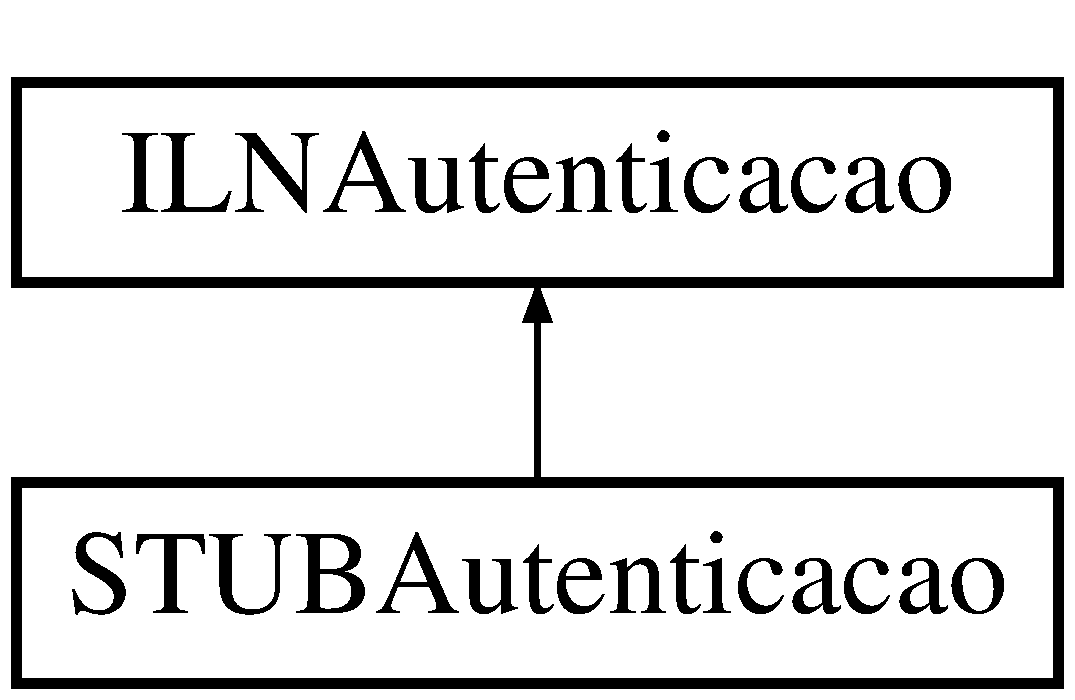
\includegraphics[height=2.000000cm]{classILNAutenticacao}
\end{center}
\end{figure}
\subsection*{Public Member Functions}
\begin{DoxyCompactItemize}
\item 
\mbox{\Hypertarget{classILNAutenticacao_ad14a6619170981ce7cfbabc5d1b38d7d}\label{classILNAutenticacao_ad14a6619170981ce7cfbabc5d1b38d7d}} 
virtual \hyperlink{classResultado}{Resultado} {\bfseries autenticar} (const \hyperlink{classApelido}{Apelido} \&, const \hyperlink{classSenha}{Senha} \&)=0  throw (runtime\+\_\+error)
\end{DoxyCompactItemize}


\subsection{Detailed Description}
Classe que representa a interface da lógica de negócio da autenticação. 

The documentation for this class was generated from the following files\+:\begin{DoxyCompactItemize}
\item 
interfaces.\+h\item 
interfaces.\+cpp\end{DoxyCompactItemize}

\hypertarget{classILNBuscarlivro}{}\section{I\+L\+N\+Buscarlivro Class Reference}
\label{classILNBuscarlivro}\index{I\+L\+N\+Buscarlivro@{I\+L\+N\+Buscarlivro}}


Classe que representa a interface da lógica de negócios da busca de livros.  




{\ttfamily \#include $<$interfaces.\+h$>$}

Inheritance diagram for I\+L\+N\+Buscarlivro\+:\begin{figure}[H]
\begin{center}
\leavevmode
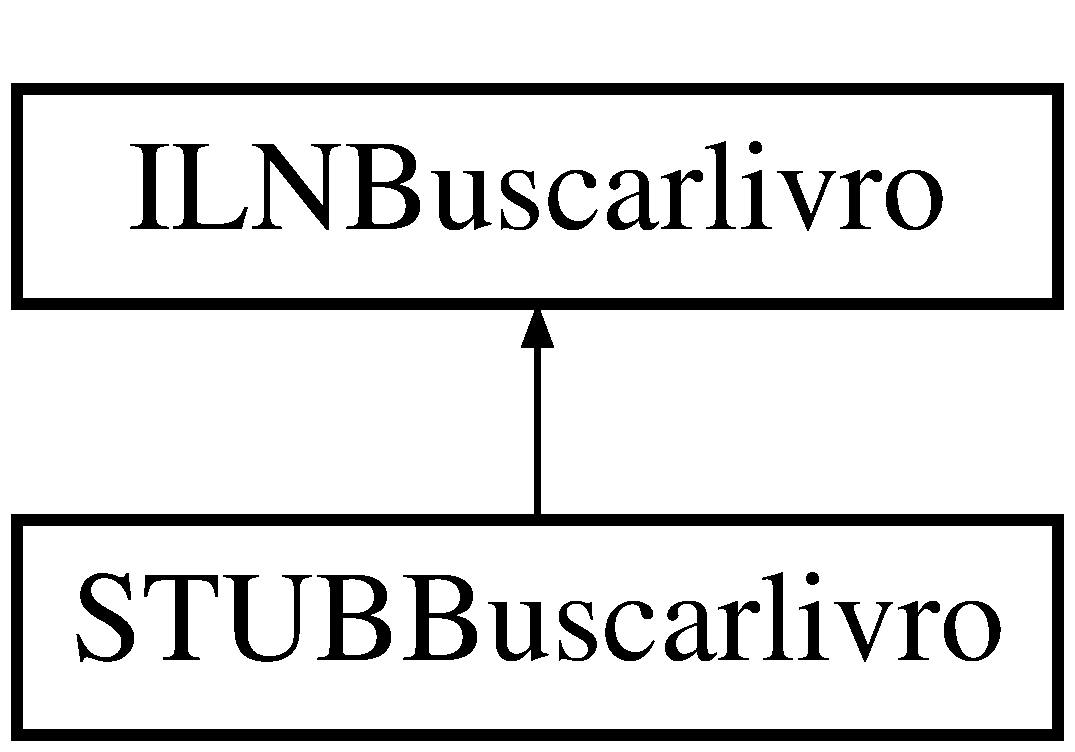
\includegraphics[height=2.000000cm]{classILNBuscarlivro}
\end{center}
\end{figure}
\subsection*{Public Member Functions}
\begin{DoxyCompactItemize}
\item 
\mbox{\Hypertarget{classILNBuscarlivro_ae04cb0c1a3461c65c07d5b97ffc0a926}\label{classILNBuscarlivro_ae04cb0c1a3461c65c07d5b97ffc0a926}} 
virtual \hyperlink{classResultado}{Resultado} {\bfseries buscarlivro} (\hyperlink{classTitulo}{Titulo} titulo)=0  throw (runtime\+\_\+error)
\end{DoxyCompactItemize}


\subsection{Detailed Description}
Classe que representa a interface da lógica de negócios da busca de livros. 

The documentation for this class was generated from the following files\+:\begin{DoxyCompactItemize}
\item 
interfaces.\+h\item 
interfaces.\+cpp\end{DoxyCompactItemize}

\hypertarget{classILNBuscarusuario}{}\section{I\+L\+N\+Buscarusuario Class Reference}
\label{classILNBuscarusuario}\index{I\+L\+N\+Buscarusuario@{I\+L\+N\+Buscarusuario}}


Classe que representa a interface da lógica de negócios da busca de usuários.  




{\ttfamily \#include $<$interfaces.\+h$>$}

Inheritance diagram for I\+L\+N\+Buscarusuario\+:\begin{figure}[H]
\begin{center}
\leavevmode
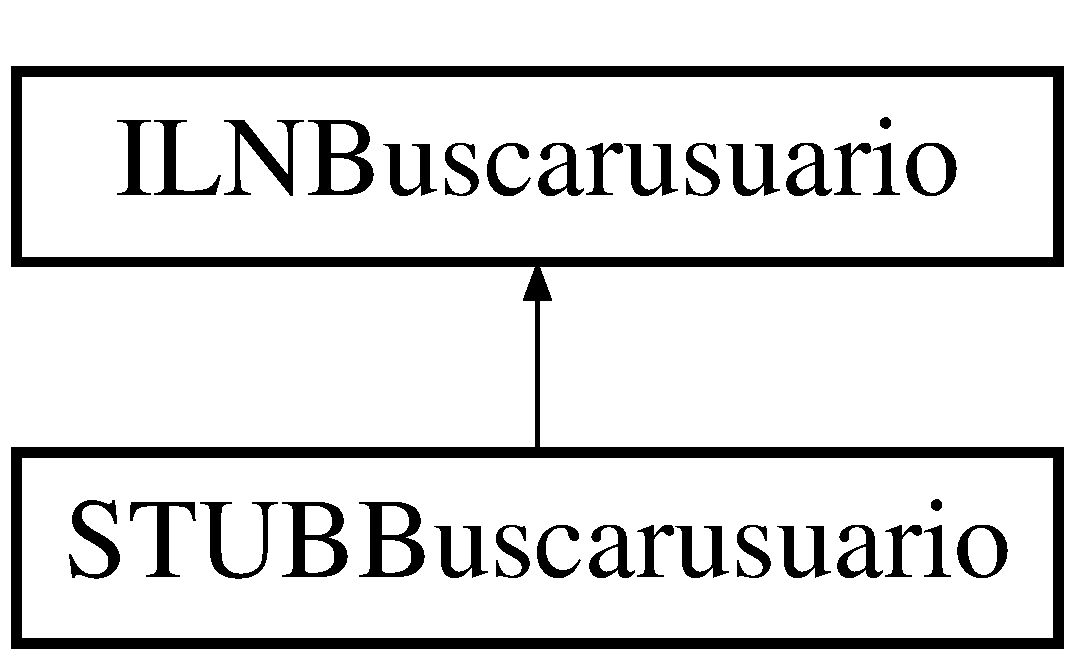
\includegraphics[height=2.000000cm]{classILNBuscarusuario}
\end{center}
\end{figure}
\subsection*{Public Member Functions}
\begin{DoxyCompactItemize}
\item 
\mbox{\Hypertarget{classILNBuscarusuario_a7880b61bd4b9d07a35609bd66c5238a2}\label{classILNBuscarusuario_a7880b61bd4b9d07a35609bd66c5238a2}} 
virtual \hyperlink{classResultado}{Resultado} {\bfseries buscarusuario} (\hyperlink{classApelido}{Apelido} apelido)=0  throw (runtime\+\_\+error)
\end{DoxyCompactItemize}


\subsection{Detailed Description}
Classe que representa a interface da lógica de negócios da busca de usuários. 

The documentation for this class was generated from the following files\+:\begin{DoxyCompactItemize}
\item 
interfaces.\+h\item 
interfaces.\+cpp\end{DoxyCompactItemize}

\hypertarget{classILNCadastro}{}\section{I\+L\+N\+Cadastro Class Reference}
\label{classILNCadastro}\index{I\+L\+N\+Cadastro@{I\+L\+N\+Cadastro}}


Classe que representa a interface da logica de negócio do cadastro.  




{\ttfamily \#include $<$interfaces.\+h$>$}

Inheritance diagram for I\+L\+N\+Cadastro\+:\begin{figure}[H]
\begin{center}
\leavevmode
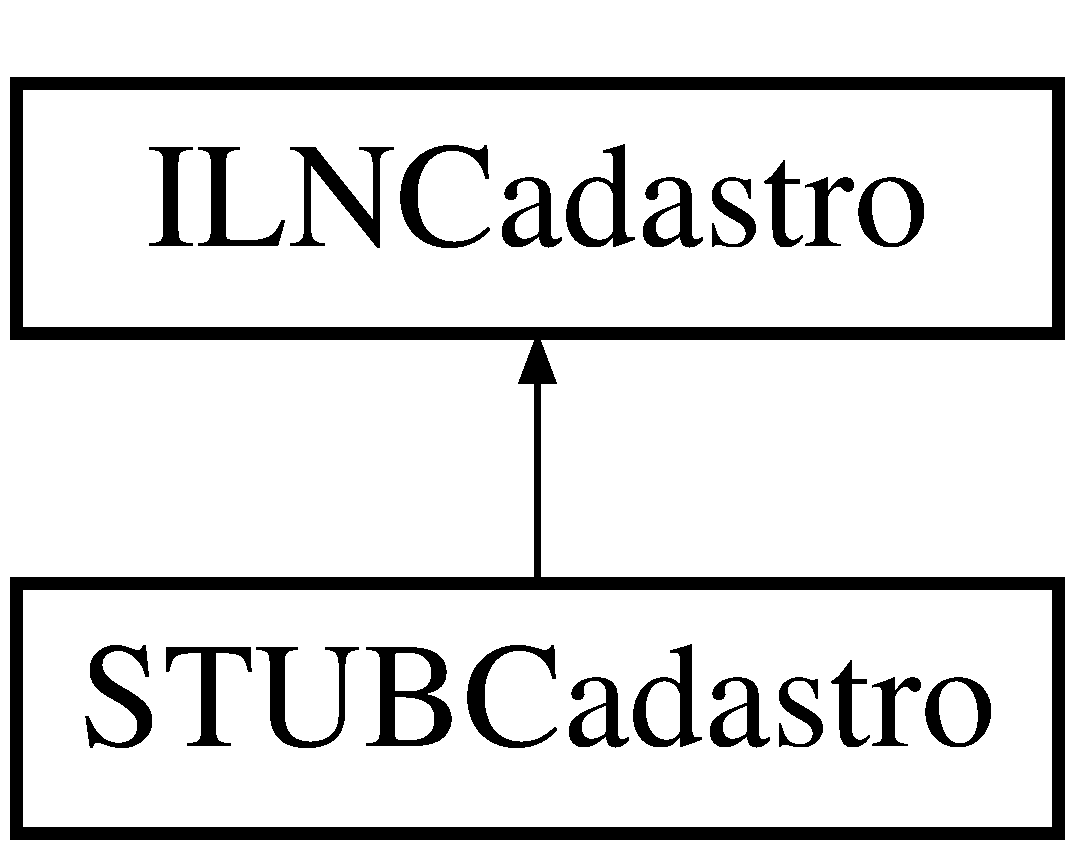
\includegraphics[height=2.000000cm]{classILNCadastro}
\end{center}
\end{figure}
\subsection*{Public Member Functions}
\begin{DoxyCompactItemize}
\item 
\mbox{\Hypertarget{classILNCadastro_a8a13b3169f6256ef2341ca13f32772b7}\label{classILNCadastro_a8a13b3169f6256ef2341ca13f32772b7}} 
virtual \hyperlink{classResultado}{Resultado} {\bfseries cadastrar} (\hyperlink{classNome}{Nome} nome, \hyperlink{classApelido}{Apelido} apelido, \hyperlink{classSenha}{Senha} senha, \hyperlink{classTelefone}{Telefone} telefone)=0  throw (runtime\+\_\+error)
\end{DoxyCompactItemize}


\subsection{Detailed Description}
Classe que representa a interface da logica de negócio do cadastro. 

The documentation for this class was generated from the following files\+:\begin{DoxyCompactItemize}
\item 
interfaces.\+h\item 
interfaces.\+cpp\end{DoxyCompactItemize}

\hypertarget{classILNCadastrolivro}{}\section{I\+L\+N\+Cadastrolivro Class Reference}
\label{classILNCadastrolivro}\index{I\+L\+N\+Cadastrolivro@{I\+L\+N\+Cadastrolivro}}


Classe que representa a interface da logica de negócio do cadastro do livro.  




{\ttfamily \#include $<$interfaces.\+h$>$}

Inheritance diagram for I\+L\+N\+Cadastrolivro\+:\begin{figure}[H]
\begin{center}
\leavevmode
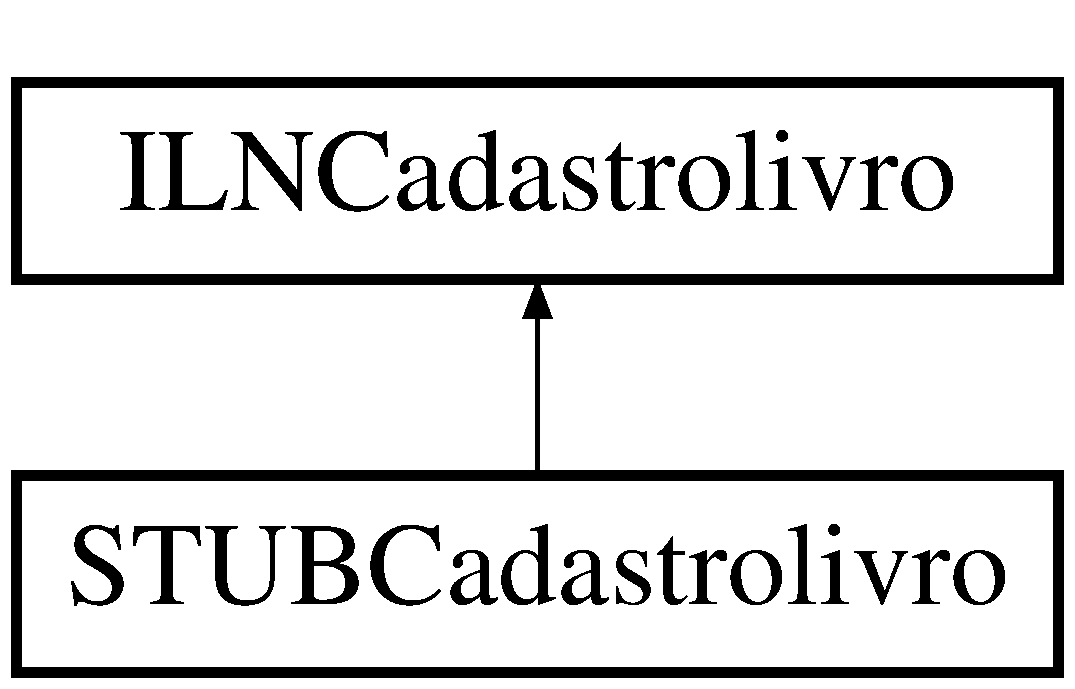
\includegraphics[height=2.000000cm]{classILNCadastrolivro}
\end{center}
\end{figure}
\subsection*{Public Member Functions}
\begin{DoxyCompactItemize}
\item 
\mbox{\Hypertarget{classILNCadastrolivro_a88ba46808fe59c8e4df1cab259e4b674}\label{classILNCadastrolivro_a88ba46808fe59c8e4df1cab259e4b674}} 
virtual \hyperlink{classResultado}{Resultado} {\bfseries cadastrarlivro} (\hyperlink{classTitulo}{Titulo} titulo, \hyperlink{classNome}{Nome} autor, \hyperlink{classData}{Data} data, \hyperlink{classCodigo}{Codigo} codigo, \hyperlink{classGenero}{Genero} genero)=0  throw (runtime\+\_\+error)
\end{DoxyCompactItemize}


\subsection{Detailed Description}
Classe que representa a interface da logica de negócio do cadastro do livro. 

The documentation for this class was generated from the following files\+:\begin{DoxyCompactItemize}
\item 
interfaces.\+h\item 
interfaces.\+cpp\end{DoxyCompactItemize}

\hypertarget{classILNComandosusuarioautenticado}{}\section{I\+L\+N\+Comandosusuarioautenticado Class Reference}
\label{classILNComandosusuarioautenticado}\index{I\+L\+N\+Comandosusuarioautenticado@{I\+L\+N\+Comandosusuarioautenticado}}


Classe que representa a interface da lógica de negócios enolvendo os comandos de um usuário autenticado.  




{\ttfamily \#include $<$interfaces.\+h$>$}

Inheritance diagram for I\+L\+N\+Comandosusuarioautenticado\+:\begin{figure}[H]
\begin{center}
\leavevmode
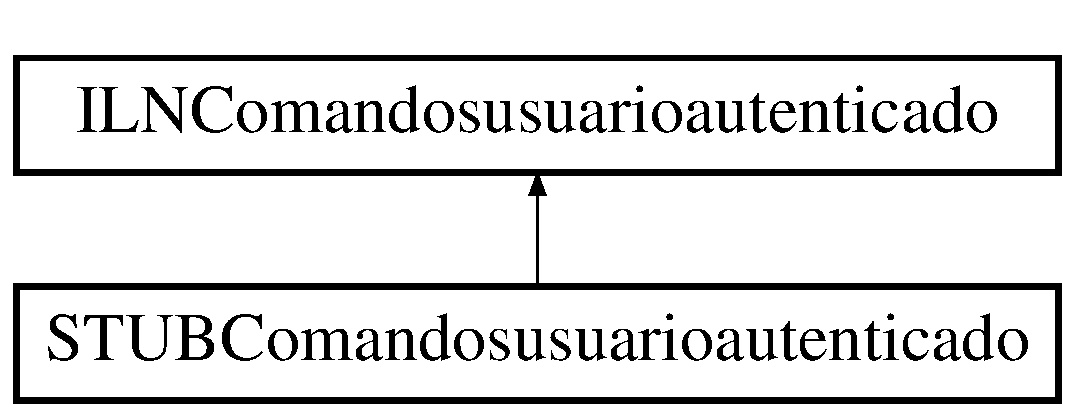
\includegraphics[height=2.000000cm]{classILNComandosusuarioautenticado}
\end{center}
\end{figure}
\subsection*{Public Member Functions}
\begin{DoxyCompactItemize}
\item 
\mbox{\Hypertarget{classILNComandosusuarioautenticado_ab2ca5ec649e35c255365036e6b01b9d3}\label{classILNComandosusuarioautenticado_ab2ca5ec649e35c255365036e6b01b9d3}} 
virtual \hyperlink{classResultado}{Resultado} {\bfseries incluir} (const \hyperlink{classTitulo}{Titulo} \&, const \hyperlink{classNome}{Nome} \&, const \hyperlink{classData}{Data} \&, const \hyperlink{classCodigo}{Codigo} \&, const \hyperlink{classGenero}{Genero} \&)=0  throw (runtime\+\_\+error)
\item 
\mbox{\Hypertarget{classILNComandosusuarioautenticado_a3aa5a13eeee0cb3e29cece7863fc4ea7}\label{classILNComandosusuarioautenticado_a3aa5a13eeee0cb3e29cece7863fc4ea7}} 
virtual \hyperlink{classResultado}{Resultado} {\bfseries remover} (const \hyperlink{classTitulo}{Titulo} \&)=0  throw (runtime\+\_\+error)
\item 
\mbox{\Hypertarget{classILNComandosusuarioautenticado_a48070d42283390450ae47e465aa81751}\label{classILNComandosusuarioautenticado_a48070d42283390450ae47e465aa81751}} 
virtual \hyperlink{classResultado}{Resultado} {\bfseries registrarresenha} (const \hyperlink{classNome}{Nome} \&, const \hyperlink{classTitulo}{Titulo} \&, const \hyperlink{classTexto}{Texto} \&)=0  throw (runtime\+\_\+error)
\item 
\mbox{\Hypertarget{classILNComandosusuarioautenticado_a38e0e08ef0a0c1e797cfe1794f3f3eda}\label{classILNComandosusuarioautenticado_a38e0e08ef0a0c1e797cfe1794f3f3eda}} 
virtual \hyperlink{classResultado}{Resultado} {\bfseries trocarlivro} (const \hyperlink{classTitulo}{Titulo} \&)=0  throw (runtime\+\_\+error)
\item 
\mbox{\Hypertarget{classILNComandosusuarioautenticado_a5c82aec8f7d5211ab0a1acc445d8f3dd}\label{classILNComandosusuarioautenticado_a5c82aec8f7d5211ab0a1acc445d8f3dd}} 
virtual \hyperlink{classResultado}{Resultado} {\bfseries buscarlivro} (const \hyperlink{classTitulo}{Titulo} \&)=0  throw (runtime\+\_\+error)
\item 
\mbox{\Hypertarget{classILNComandosusuarioautenticado_a7e33d964a8961cd305b67e2f6184b9a6}\label{classILNComandosusuarioautenticado_a7e33d964a8961cd305b67e2f6184b9a6}} 
virtual \hyperlink{classResultado}{Resultado} {\bfseries buscarusuario} (const \hyperlink{classApelido}{Apelido} \&)=0  throw (runtime\+\_\+error)
\end{DoxyCompactItemize}


\subsection{Detailed Description}
Classe que representa a interface da lógica de negócios enolvendo os comandos de um usuário autenticado. 

The documentation for this class was generated from the following files\+:\begin{DoxyCompactItemize}
\item 
interfaces.\+h\item 
interfaces.\+cpp\end{DoxyCompactItemize}

\hypertarget{classILNRegistroresenha}{}\section{I\+L\+N\+Registroresenha Class Reference}
\label{classILNRegistroresenha}\index{I\+L\+N\+Registroresenha@{I\+L\+N\+Registroresenha}}


Classe que representa a interface da lógica de negócios do registro de resenhas.  




{\ttfamily \#include $<$interfaces.\+h$>$}

Inheritance diagram for I\+L\+N\+Registroresenha\+:\begin{figure}[H]
\begin{center}
\leavevmode
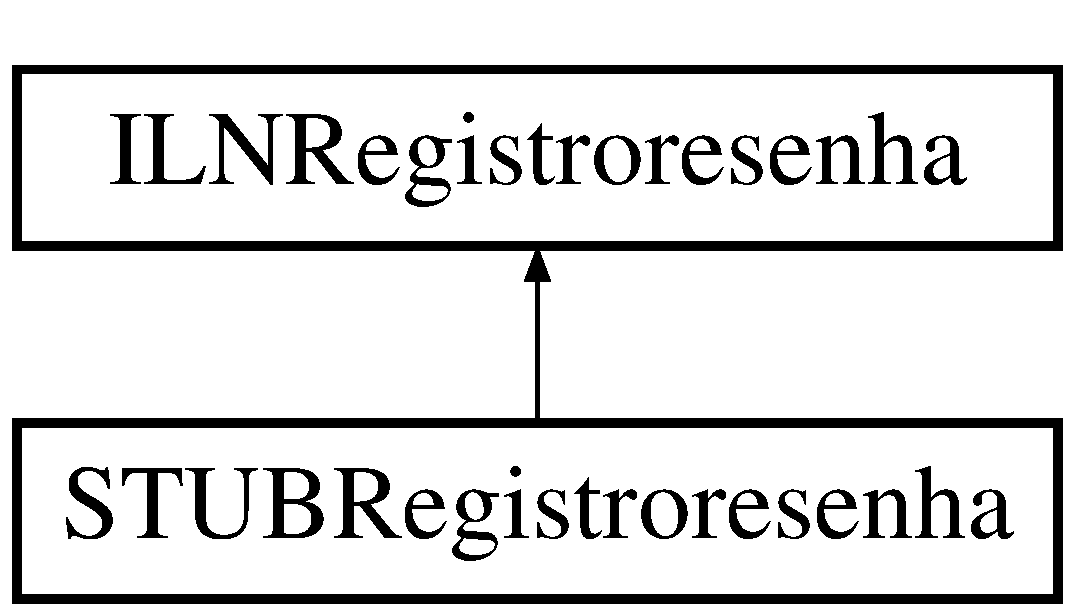
\includegraphics[height=2.000000cm]{classILNRegistroresenha}
\end{center}
\end{figure}
\subsection*{Public Member Functions}
\begin{DoxyCompactItemize}
\item 
\mbox{\Hypertarget{classILNRegistroresenha_a9949a5e396cb177a8f135f6734b517c1}\label{classILNRegistroresenha_a9949a5e396cb177a8f135f6734b517c1}} 
virtual \hyperlink{classResultado}{Resultado} {\bfseries registrarresenha} (const \hyperlink{classNome}{Nome} \&, const \hyperlink{classTitulo}{Titulo} \&, const \hyperlink{classTexto}{Texto} \&)=0  throw (runtime\+\_\+error)
\end{DoxyCompactItemize}


\subsection{Detailed Description}
Classe que representa a interface da lógica de negócios do registro de resenhas. 

The documentation for this class was generated from the following files\+:\begin{DoxyCompactItemize}
\item 
interfaces.\+h\item 
interfaces.\+cpp\end{DoxyCompactItemize}

\hypertarget{classILNTrocarlivro}{}\section{I\+L\+N\+Trocarlivro Class Reference}
\label{classILNTrocarlivro}\index{I\+L\+N\+Trocarlivro@{I\+L\+N\+Trocarlivro}}


Classe que representa a interface da lógica de negócios da troca de livros.  




{\ttfamily \#include $<$interfaces.\+h$>$}

Inheritance diagram for I\+L\+N\+Trocarlivro\+:\begin{figure}[H]
\begin{center}
\leavevmode
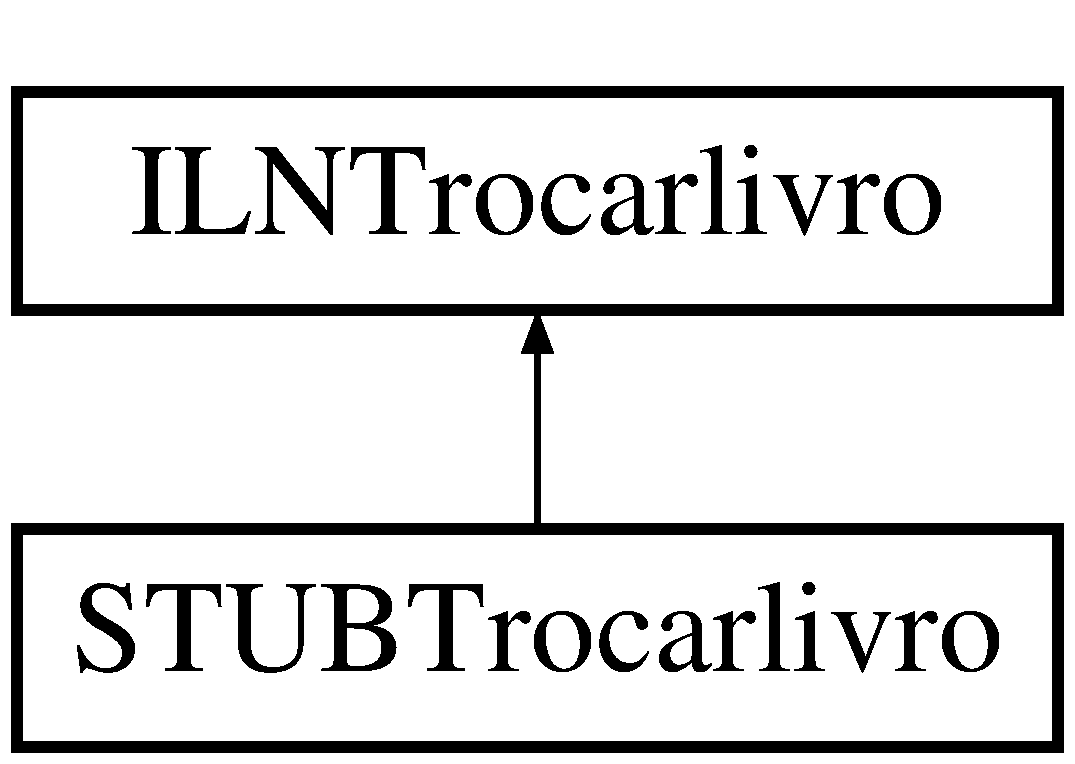
\includegraphics[height=2.000000cm]{classILNTrocarlivro}
\end{center}
\end{figure}
\subsection*{Public Member Functions}
\begin{DoxyCompactItemize}
\item 
\mbox{\Hypertarget{classILNTrocarlivro_a01c734c2dde5fd2ed32b0bb873afc4a0}\label{classILNTrocarlivro_a01c734c2dde5fd2ed32b0bb873afc4a0}} 
virtual \hyperlink{classResultado}{Resultado} {\bfseries trocarlivro} (const \hyperlink{classTitulo}{Titulo} \&)=0  throw (runtime\+\_\+error)
\end{DoxyCompactItemize}


\subsection{Detailed Description}
Classe que representa a interface da lógica de negócios da troca de livros. 

The documentation for this class was generated from the following files\+:\begin{DoxyCompactItemize}
\item 
interfaces.\+h\item 
interfaces.\+cpp\end{DoxyCompactItemize}

\hypertarget{classIUAutenticacao}{}\section{I\+U\+Autenticacao Class Reference}
\label{classIUAutenticacao}\index{I\+U\+Autenticacao@{I\+U\+Autenticacao}}


Classe que representa a interface de usuario da autenticação.  




{\ttfamily \#include $<$interfaces.\+h$>$}

Inheritance diagram for I\+U\+Autenticacao\+:\begin{figure}[H]
\begin{center}
\leavevmode
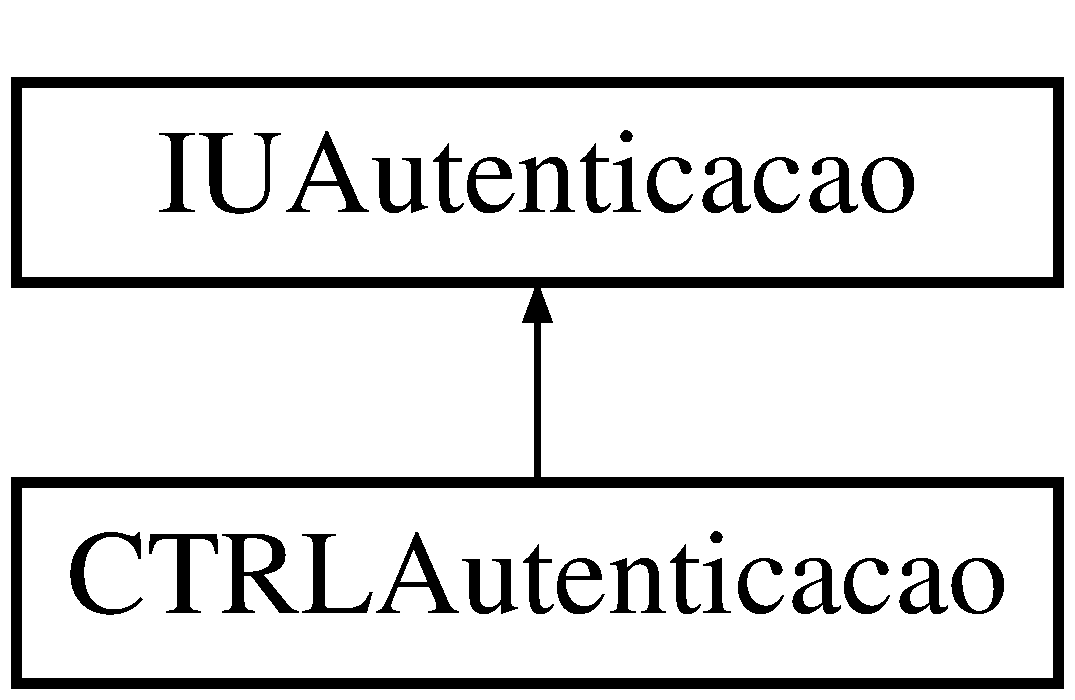
\includegraphics[height=2.000000cm]{classIUAutenticacao}
\end{center}
\end{figure}
\subsection*{Public Member Functions}
\begin{DoxyCompactItemize}
\item 
\mbox{\Hypertarget{classIUAutenticacao_aad1e46db9061a785e3462a1f78d032f9}\label{classIUAutenticacao_aad1e46db9061a785e3462a1f78d032f9}} 
virtual \hyperlink{classResultado}{Resultado} {\bfseries autenticar} (\hyperlink{classUsuario}{Usuario} $\ast$$\ast$)=0  throw (runtime\+\_\+error)
\item 
\mbox{\Hypertarget{classIUAutenticacao_a86f10a01262f1ef6a6944bdb71aa6a88}\label{classIUAutenticacao_a86f10a01262f1ef6a6944bdb71aa6a88}} 
virtual void {\bfseries set\+Container} (\hyperlink{classContainerUsuario}{Container\+Usuario} $\ast$)=0
\end{DoxyCompactItemize}


\subsection{Detailed Description}
Classe que representa a interface de usuario da autenticação. 

The documentation for this class was generated from the following files\+:\begin{DoxyCompactItemize}
\item 
interfaces.\+h\item 
interfaces.\+cpp\end{DoxyCompactItemize}

\hypertarget{classIUBuscarlivro}{}\section{I\+U\+Buscarlivro Class Reference}
\label{classIUBuscarlivro}\index{I\+U\+Buscarlivro@{I\+U\+Buscarlivro}}


Classe que representa a interface de usuario da busca de livros.  




{\ttfamily \#include $<$interfaces.\+h$>$}

Inheritance diagram for I\+U\+Buscarlivro\+:\begin{figure}[H]
\begin{center}
\leavevmode
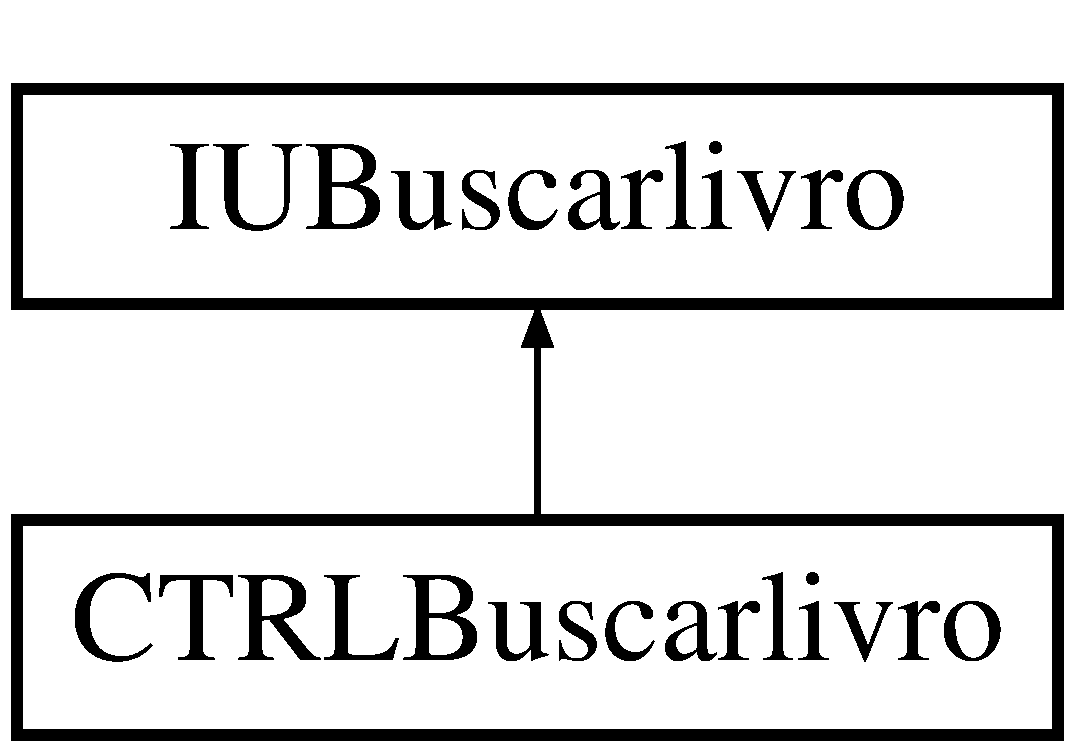
\includegraphics[height=2.000000cm]{classIUBuscarlivro}
\end{center}
\end{figure}
\subsection*{Public Member Functions}
\begin{DoxyCompactItemize}
\item 
\mbox{\Hypertarget{classIUBuscarlivro_ae52dbdd65e898fcb0173895117cb62c7}\label{classIUBuscarlivro_ae52dbdd65e898fcb0173895117cb62c7}} 
virtual \hyperlink{classResultado}{Resultado} {\bfseries buscarlivro} ()=0  throw (runtime\+\_\+error)
\item 
\mbox{\Hypertarget{classIUBuscarlivro_abbb9b7eb41b4ec7352fecb9376ec0207}\label{classIUBuscarlivro_abbb9b7eb41b4ec7352fecb9376ec0207}} 
virtual void {\bfseries set\+Cntr\+L\+N\+Buscarlivro} (\hyperlink{classILNBuscarlivro}{I\+L\+N\+Buscarlivro} $\ast$)=0
\end{DoxyCompactItemize}


\subsection{Detailed Description}
Classe que representa a interface de usuario da busca de livros. 

The documentation for this class was generated from the following files\+:\begin{DoxyCompactItemize}
\item 
interfaces.\+h\item 
interfaces.\+cpp\end{DoxyCompactItemize}

\hypertarget{classIUBuscarusuario}{}\section{I\+U\+Buscarusuario Class Reference}
\label{classIUBuscarusuario}\index{I\+U\+Buscarusuario@{I\+U\+Buscarusuario}}


Classe que representa a interface de usuario da busca de usuários.  




{\ttfamily \#include $<$interfaces.\+h$>$}

Inheritance diagram for I\+U\+Buscarusuario\+:\begin{figure}[H]
\begin{center}
\leavevmode
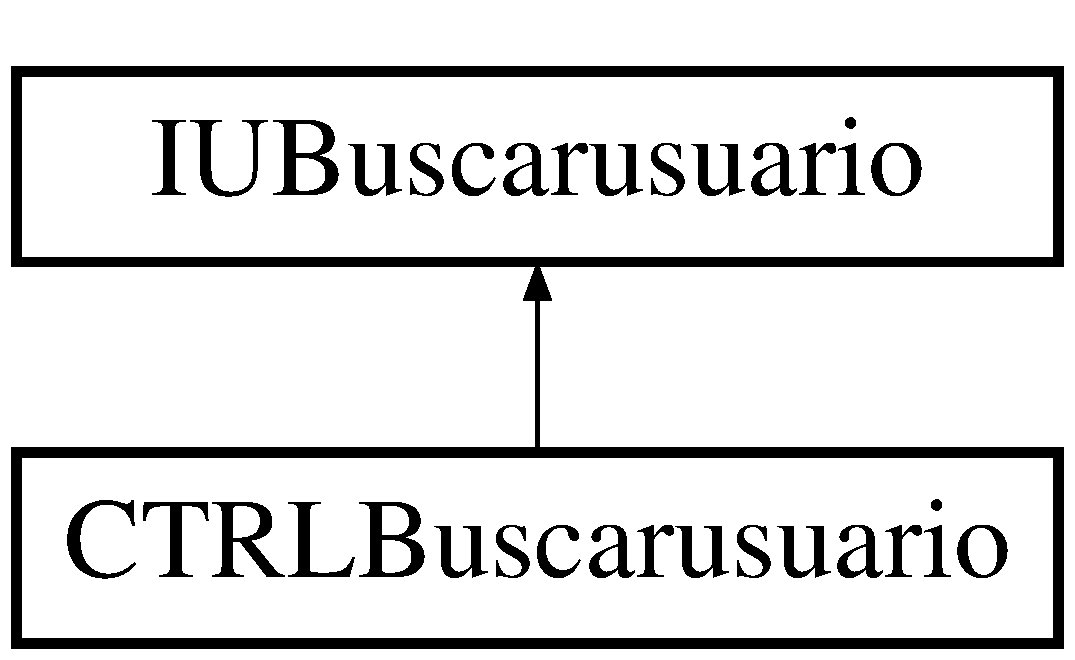
\includegraphics[height=2.000000cm]{classIUBuscarusuario}
\end{center}
\end{figure}
\subsection*{Public Member Functions}
\begin{DoxyCompactItemize}
\item 
\mbox{\Hypertarget{classIUBuscarusuario_a325a581f5e61a973ced408613a12af0e}\label{classIUBuscarusuario_a325a581f5e61a973ced408613a12af0e}} 
virtual \hyperlink{classResultado}{Resultado} {\bfseries buscarusuario} ()=0  throw (runtime\+\_\+error)
\item 
\mbox{\Hypertarget{classIUBuscarusuario_acee43910719a0e8b0f70ee1f0c189535}\label{classIUBuscarusuario_acee43910719a0e8b0f70ee1f0c189535}} 
virtual void {\bfseries set\+Container} (\hyperlink{classContainerUsuario}{Container\+Usuario} $\ast$)=0
\end{DoxyCompactItemize}


\subsection{Detailed Description}
Classe que representa a interface de usuario da busca de usuários. 

The documentation for this class was generated from the following files\+:\begin{DoxyCompactItemize}
\item 
interfaces.\+h\item 
interfaces.\+cpp\end{DoxyCompactItemize}

\hypertarget{classIUCadastro}{}\section{I\+U\+Cadastro Class Reference}
\label{classIUCadastro}\index{I\+U\+Cadastro@{I\+U\+Cadastro}}


Classe que representa a interface de usuario do cadastro.  




{\ttfamily \#include $<$interfaces.\+h$>$}

Inheritance diagram for I\+U\+Cadastro\+:\begin{figure}[H]
\begin{center}
\leavevmode
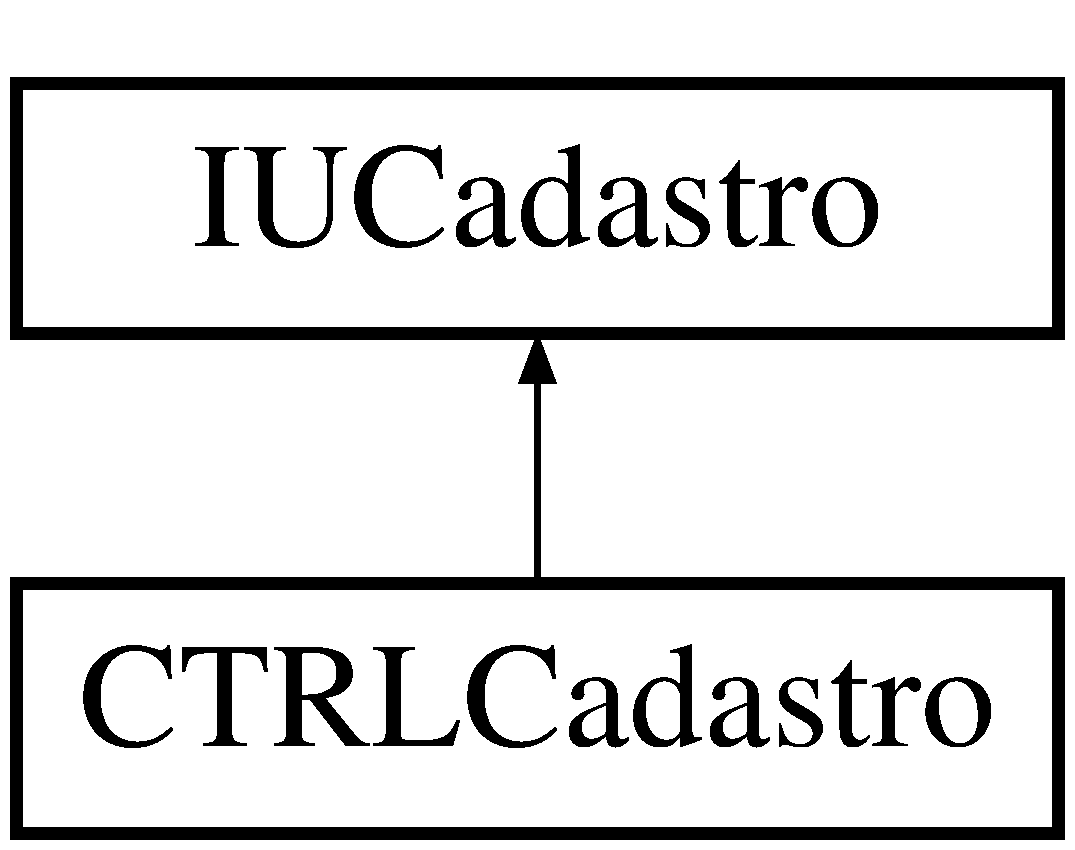
\includegraphics[height=2.000000cm]{classIUCadastro}
\end{center}
\end{figure}
\subsection*{Public Member Functions}
\begin{DoxyCompactItemize}
\item 
\mbox{\Hypertarget{classIUCadastro_af4089cca946d856abae69b931a1dc1e8}\label{classIUCadastro_af4089cca946d856abae69b931a1dc1e8}} 
virtual \hyperlink{classResultado}{Resultado} {\bfseries cadastrar} ()=0  throw (runtime\+\_\+error)
\item 
\mbox{\Hypertarget{classIUCadastro_a50128c18e84b837c6f50aaa6f898bf34}\label{classIUCadastro_a50128c18e84b837c6f50aaa6f898bf34}} 
virtual void {\bfseries set\+Container} (\hyperlink{classContainerUsuario}{Container\+Usuario} $\ast$)=0
\end{DoxyCompactItemize}


\subsection{Detailed Description}
Classe que representa a interface de usuario do cadastro. 

The documentation for this class was generated from the following files\+:\begin{DoxyCompactItemize}
\item 
interfaces.\+h\item 
interfaces.\+cpp\end{DoxyCompactItemize}

\hypertarget{classIUCadastrolivro}{}\section{I\+U\+Cadastrolivro Class Reference}
\label{classIUCadastrolivro}\index{I\+U\+Cadastrolivro@{I\+U\+Cadastrolivro}}


Classe que representa a interface de usuario do cadastro do livro.  




{\ttfamily \#include $<$interfaces.\+h$>$}

Inheritance diagram for I\+U\+Cadastrolivro\+:\begin{figure}[H]
\begin{center}
\leavevmode
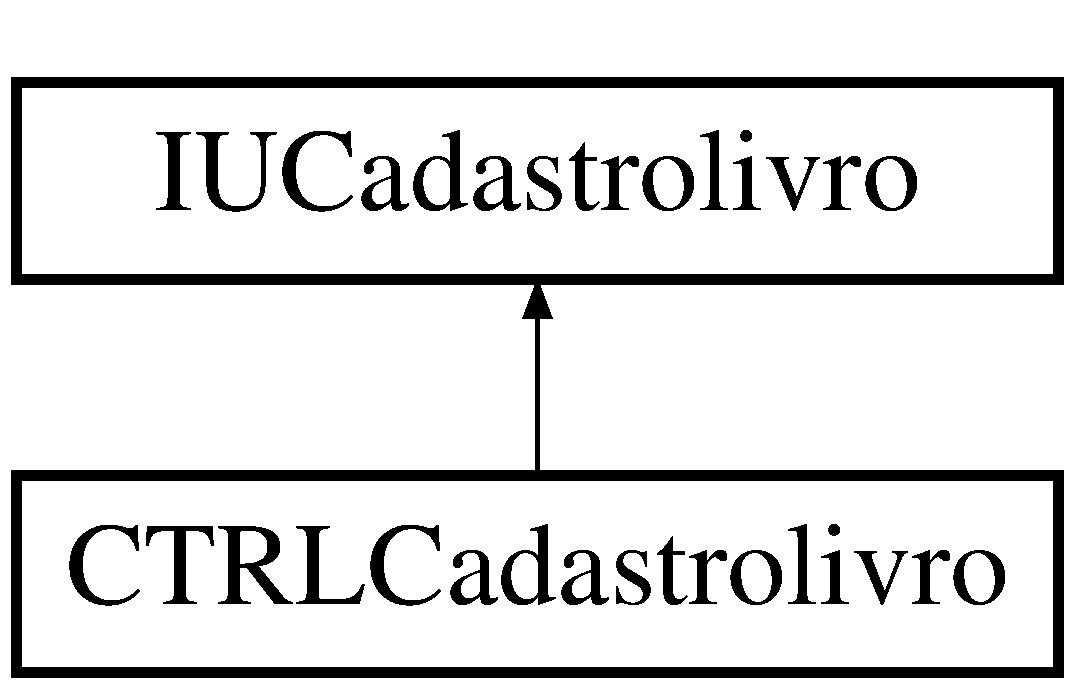
\includegraphics[height=2.000000cm]{classIUCadastrolivro}
\end{center}
\end{figure}
\subsection*{Public Member Functions}
\begin{DoxyCompactItemize}
\item 
\mbox{\Hypertarget{classIUCadastrolivro_a356b23a58950960453d24732018432e1}\label{classIUCadastrolivro_a356b23a58950960453d24732018432e1}} 
virtual \hyperlink{classResultado}{Resultado} {\bfseries cadastrarlivro} ()=0  throw (runtime\+\_\+error)
\item 
\mbox{\Hypertarget{classIUCadastrolivro_a7e660ae3e25cb51040f80a0c422b42d7}\label{classIUCadastrolivro_a7e660ae3e25cb51040f80a0c422b42d7}} 
virtual void {\bfseries set\+Cntr\+L\+N\+Cadastrolivro} (\hyperlink{classILNCadastrolivro}{I\+L\+N\+Cadastrolivro} $\ast$)=0
\end{DoxyCompactItemize}


\subsection{Detailed Description}
Classe que representa a interface de usuario do cadastro do livro. 

The documentation for this class was generated from the following files\+:\begin{DoxyCompactItemize}
\item 
interfaces.\+h\item 
interfaces.\+cpp\end{DoxyCompactItemize}

\hypertarget{classIUComandosusuarioautenticado}{}\section{I\+U\+Comandosusuarioautenticado Class Reference}
\label{classIUComandosusuarioautenticado}\index{I\+U\+Comandosusuarioautenticado@{I\+U\+Comandosusuarioautenticado}}


Classe que representa a interface de usuario dos comandos de um usuário autenticado.  




{\ttfamily \#include $<$interfaces.\+h$>$}

Inheritance diagram for I\+U\+Comandosusuarioautenticado\+:\begin{figure}[H]
\begin{center}
\leavevmode
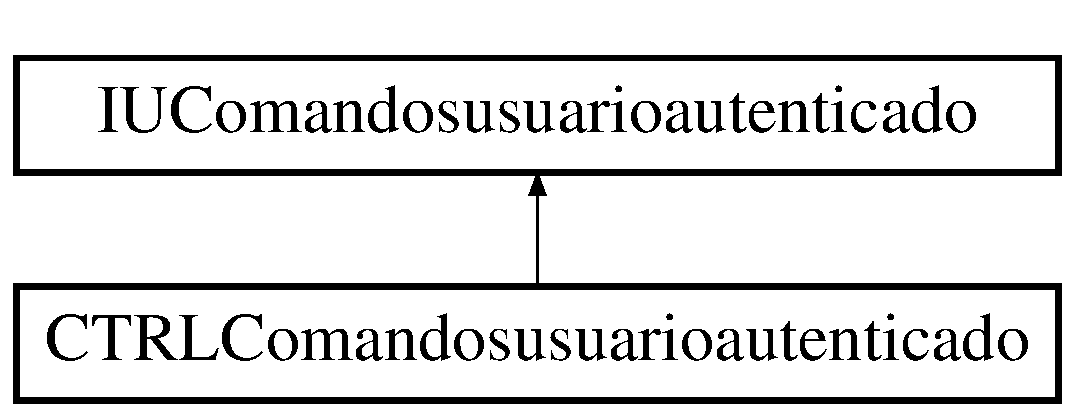
\includegraphics[height=2.000000cm]{classIUComandosusuarioautenticado}
\end{center}
\end{figure}
\subsection*{Public Member Functions}
\begin{DoxyCompactItemize}
\item 
\mbox{\Hypertarget{classIUComandosusuarioautenticado_a7c799f39789df35026e6a712e912e01a}\label{classIUComandosusuarioautenticado_a7c799f39789df35026e6a712e912e01a}} 
virtual void {\bfseries comandosusuarioautenticado} ()=0  throw (runtime\+\_\+error)
\item 
\mbox{\Hypertarget{classIUComandosusuarioautenticado_adeedafbe26781918a1fb7471a721e0b2}\label{classIUComandosusuarioautenticado_adeedafbe26781918a1fb7471a721e0b2}} 
virtual void {\bfseries set\+Cntr\+L\+N\+Comandosusuarioautenticado} (\hyperlink{classILNComandosusuarioautenticado}{I\+L\+N\+Comandosusuarioautenticado} $\ast$)=0
\end{DoxyCompactItemize}


\subsection{Detailed Description}
Classe que representa a interface de usuario dos comandos de um usuário autenticado. 

The documentation for this class was generated from the following files\+:\begin{DoxyCompactItemize}
\item 
interfaces.\+h\item 
interfaces.\+cpp\end{DoxyCompactItemize}

\hypertarget{classIURegistroresenha}{}\section{I\+U\+Registroresenha Class Reference}
\label{classIURegistroresenha}\index{I\+U\+Registroresenha@{I\+U\+Registroresenha}}


Classe que representa a interface de usuario do registro de resenhas.  




{\ttfamily \#include $<$interfaces.\+h$>$}

Inheritance diagram for I\+U\+Registroresenha\+:\begin{figure}[H]
\begin{center}
\leavevmode
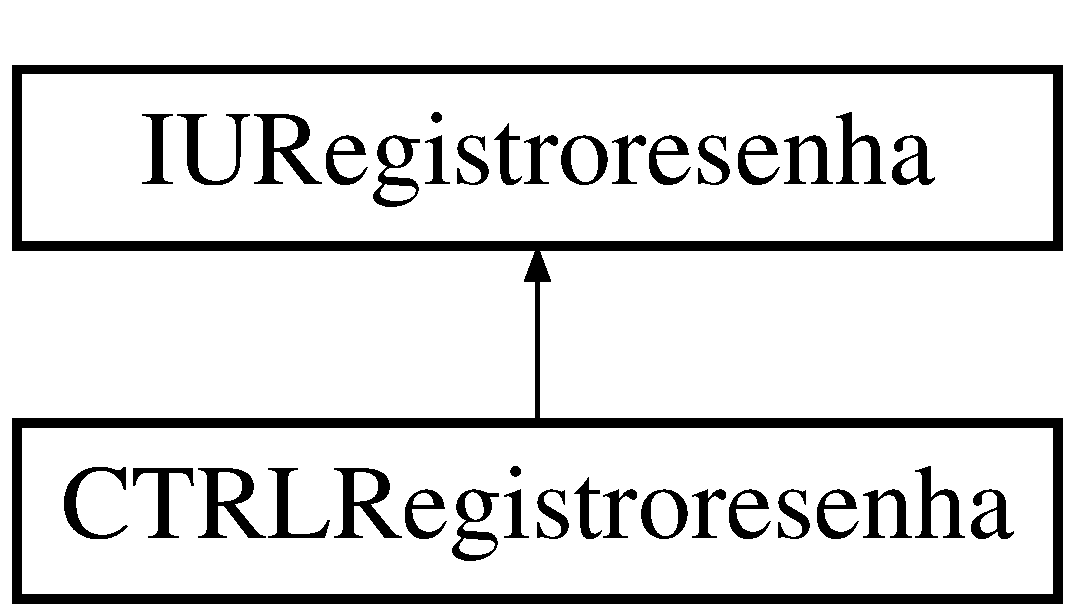
\includegraphics[height=2.000000cm]{classIURegistroresenha}
\end{center}
\end{figure}
\subsection*{Public Member Functions}
\begin{DoxyCompactItemize}
\item 
\mbox{\Hypertarget{classIURegistroresenha_abf6819abf4508a0b9df02e089a2cbba1}\label{classIURegistroresenha_abf6819abf4508a0b9df02e089a2cbba1}} 
virtual \hyperlink{classResultado}{Resultado} {\bfseries registrarresenha} ()=0  throw (runtime\+\_\+error)
\item 
\mbox{\Hypertarget{classIURegistroresenha_a4cff1619add6e6cb7081b195ce385957}\label{classIURegistroresenha_a4cff1619add6e6cb7081b195ce385957}} 
virtual void {\bfseries set\+Cntr\+L\+N\+Registroresenha} (\hyperlink{classILNRegistroresenha}{I\+L\+N\+Registroresenha} $\ast$)=0
\end{DoxyCompactItemize}


\subsection{Detailed Description}
Classe que representa a interface de usuario do registro de resenhas. 

The documentation for this class was generated from the following files\+:\begin{DoxyCompactItemize}
\item 
interfaces.\+h\item 
interfaces.\+cpp\end{DoxyCompactItemize}

\hypertarget{classIUTrocarlivro}{}\section{I\+U\+Trocarlivro Class Reference}
\label{classIUTrocarlivro}\index{I\+U\+Trocarlivro@{I\+U\+Trocarlivro}}


Classe que representa a interface de usuario da troca de livros.  




{\ttfamily \#include $<$interfaces.\+h$>$}

Inheritance diagram for I\+U\+Trocarlivro\+:\begin{figure}[H]
\begin{center}
\leavevmode
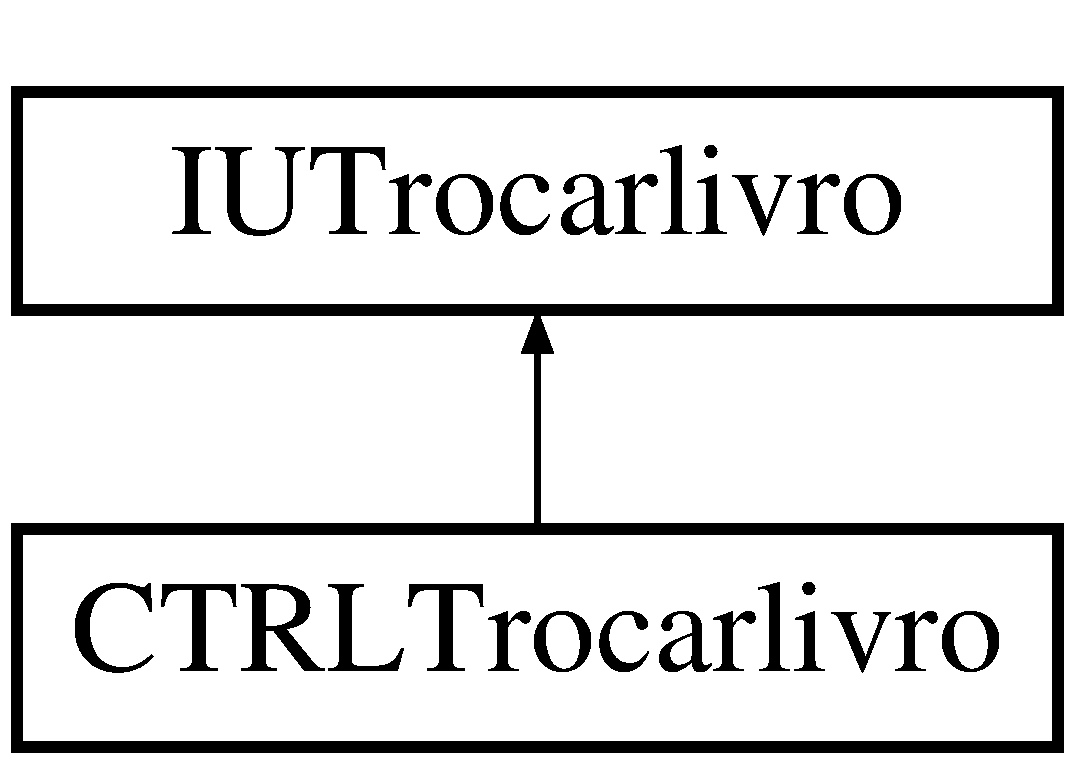
\includegraphics[height=2.000000cm]{classIUTrocarlivro}
\end{center}
\end{figure}
\subsection*{Public Member Functions}
\begin{DoxyCompactItemize}
\item 
\mbox{\Hypertarget{classIUTrocarlivro_aedae37ad25cc9af5a18fcb8afd5f987f}\label{classIUTrocarlivro_aedae37ad25cc9af5a18fcb8afd5f987f}} 
virtual \hyperlink{classResultado}{Resultado} {\bfseries trocarlivro} ()=0  throw (runtime\+\_\+error)
\item 
\mbox{\Hypertarget{classIUTrocarlivro_acfae9cd5977eb34ae9fbe0bbe70c3025}\label{classIUTrocarlivro_acfae9cd5977eb34ae9fbe0bbe70c3025}} 
virtual void {\bfseries set\+Container} (\hyperlink{classContainerLivro}{Container\+Livro} $\ast$)=0
\end{DoxyCompactItemize}


\subsection{Detailed Description}
Classe que representa a interface de usuario da troca de livros. 

The documentation for this class was generated from the following files\+:\begin{DoxyCompactItemize}
\item 
interfaces.\+h\item 
interfaces.\+cpp\end{DoxyCompactItemize}

\hypertarget{classLivro}{}\section{Livro Class Reference}
\label{classLivro}\index{Livro@{Livro}}


Classe que representa a entidade \hyperlink{classLivro}{Livro}, esta que contém os atributos\+: título, autor, data, código e gênero.  




{\ttfamily \#include $<$entidades.\+h$>$}

\subsection*{Public Member Functions}
\begin{DoxyCompactItemize}
\item 
void \hyperlink{classLivro_adbae26ce6938e1f56ed6d88b458351c7}{set\+Titulo} (string titulo)  throw (invalid\+\_\+argument)
\item 
string \hyperlink{classLivro_a4b4e2e74d4fa1a0e6e9a4d6c05dc3bd4}{get\+Titulo} () const
\item 
void \hyperlink{classLivro_ab6979584fef48cc9b2ca4dc0359dd69d}{set\+Autor} (string autor)  throw (invalid\+\_\+argument)
\item 
string \hyperlink{classLivro_ae8f2ea7e82a3ddd33e1d0e242c43f3e5}{get\+Autor} () const
\item 
void \hyperlink{classLivro_a073f7124564707c5c36e9a44448aa13a}{set\+Data} (string data)  throw (invalid\+\_\+argument)
\item 
string \hyperlink{classLivro_aaf7d614049f22c09631bae2a5f83c16a}{get\+Data} () const
\item 
void \hyperlink{classLivro_a814d21b9fc0e35f974fcd7739082ea58}{set\+Codigo} (string codigo)  throw (invalid\+\_\+argument)
\item 
string \hyperlink{classLivro_ac0bf6014dae1a0a3cb15ffac8b886f13}{get\+Codigo} () const
\item 
void \hyperlink{classLivro_a642383a02f6a1dac3f69de8ac80184e7}{set\+Genero} (string genero)  throw (invalid\+\_\+argument)
\item 
string \hyperlink{classLivro_a00b6085b059571efab6d29630cf95a50}{get\+Genero} () const
\end{DoxyCompactItemize}


\subsection{Detailed Description}
Classe que representa a entidade \hyperlink{classLivro}{Livro}, esta que contém os atributos\+: título, autor, data, código e gênero. 

\subsection{Member Function Documentation}
\mbox{\Hypertarget{classLivro_ae8f2ea7e82a3ddd33e1d0e242c43f3e5}\label{classLivro_ae8f2ea7e82a3ddd33e1d0e242c43f3e5}} 
\index{Livro@{Livro}!get\+Autor@{get\+Autor}}
\index{get\+Autor@{get\+Autor}!Livro@{Livro}}
\subsubsection{\texorpdfstring{get\+Autor()}{getAutor()}}
{\footnotesize\ttfamily string Livro\+::get\+Autor (\begin{DoxyParamCaption}{ }\end{DoxyParamCaption}) const\hspace{0.3cm}{\ttfamily [inline]}}

Método responsável por retornar o autor do livro. Retorna uma string. \mbox{\Hypertarget{classLivro_ac0bf6014dae1a0a3cb15ffac8b886f13}\label{classLivro_ac0bf6014dae1a0a3cb15ffac8b886f13}} 
\index{Livro@{Livro}!get\+Codigo@{get\+Codigo}}
\index{get\+Codigo@{get\+Codigo}!Livro@{Livro}}
\subsubsection{\texorpdfstring{get\+Codigo()}{getCodigo()}}
{\footnotesize\ttfamily string Livro\+::get\+Codigo (\begin{DoxyParamCaption}{ }\end{DoxyParamCaption}) const\hspace{0.3cm}{\ttfamily [inline]}}

Método responsável por retornar o código do livro. Retorna uma string. \mbox{\Hypertarget{classLivro_aaf7d614049f22c09631bae2a5f83c16a}\label{classLivro_aaf7d614049f22c09631bae2a5f83c16a}} 
\index{Livro@{Livro}!get\+Data@{get\+Data}}
\index{get\+Data@{get\+Data}!Livro@{Livro}}
\subsubsection{\texorpdfstring{get\+Data()}{getData()}}
{\footnotesize\ttfamily string Livro\+::get\+Data (\begin{DoxyParamCaption}{ }\end{DoxyParamCaption}) const\hspace{0.3cm}{\ttfamily [inline]}}

Método responsável por retornar a data de publicação do livro. Retorna uma string. \mbox{\Hypertarget{classLivro_a00b6085b059571efab6d29630cf95a50}\label{classLivro_a00b6085b059571efab6d29630cf95a50}} 
\index{Livro@{Livro}!get\+Genero@{get\+Genero}}
\index{get\+Genero@{get\+Genero}!Livro@{Livro}}
\subsubsection{\texorpdfstring{get\+Genero()}{getGenero()}}
{\footnotesize\ttfamily string Livro\+::get\+Genero (\begin{DoxyParamCaption}{ }\end{DoxyParamCaption}) const\hspace{0.3cm}{\ttfamily [inline]}}

Método responsável por retornar o gênero literário do livro. Retorna uma string. \mbox{\Hypertarget{classLivro_a4b4e2e74d4fa1a0e6e9a4d6c05dc3bd4}\label{classLivro_a4b4e2e74d4fa1a0e6e9a4d6c05dc3bd4}} 
\index{Livro@{Livro}!get\+Titulo@{get\+Titulo}}
\index{get\+Titulo@{get\+Titulo}!Livro@{Livro}}
\subsubsection{\texorpdfstring{get\+Titulo()}{getTitulo()}}
{\footnotesize\ttfamily string Livro\+::get\+Titulo (\begin{DoxyParamCaption}{ }\end{DoxyParamCaption}) const\hspace{0.3cm}{\ttfamily [inline]}}

Método responsável por retornar o título do livro. Retorna uma string. \mbox{\Hypertarget{classLivro_ab6979584fef48cc9b2ca4dc0359dd69d}\label{classLivro_ab6979584fef48cc9b2ca4dc0359dd69d}} 
\index{Livro@{Livro}!set\+Autor@{set\+Autor}}
\index{set\+Autor@{set\+Autor}!Livro@{Livro}}
\subsubsection{\texorpdfstring{set\+Autor()}{setAutor()}}
{\footnotesize\ttfamily void Livro\+::set\+Autor (\begin{DoxyParamCaption}\item[{string}]{autor }\end{DoxyParamCaption}) throw  invalid\+\_\+argument) \hspace{0.3cm}{\ttfamily [inline]}}

Método responsável por armazenar o autor de determinado livro. É necessário uma string como entrada e lança uma exceção caso esta não seja válida. \mbox{\Hypertarget{classLivro_a814d21b9fc0e35f974fcd7739082ea58}\label{classLivro_a814d21b9fc0e35f974fcd7739082ea58}} 
\index{Livro@{Livro}!set\+Codigo@{set\+Codigo}}
\index{set\+Codigo@{set\+Codigo}!Livro@{Livro}}
\subsubsection{\texorpdfstring{set\+Codigo()}{setCodigo()}}
{\footnotesize\ttfamily void Livro\+::set\+Codigo (\begin{DoxyParamCaption}\item[{string}]{codigo }\end{DoxyParamCaption}) throw  invalid\+\_\+argument) \hspace{0.3cm}{\ttfamily [inline]}}

Método responsável por armazenar o código de determinado livro. É necessário uma string como entrada e lança uma exceção caso esta não seja válida. \mbox{\Hypertarget{classLivro_a073f7124564707c5c36e9a44448aa13a}\label{classLivro_a073f7124564707c5c36e9a44448aa13a}} 
\index{Livro@{Livro}!set\+Data@{set\+Data}}
\index{set\+Data@{set\+Data}!Livro@{Livro}}
\subsubsection{\texorpdfstring{set\+Data()}{setData()}}
{\footnotesize\ttfamily void Livro\+::set\+Data (\begin{DoxyParamCaption}\item[{string}]{data }\end{DoxyParamCaption}) throw  invalid\+\_\+argument) \hspace{0.3cm}{\ttfamily [inline]}}

Método responsável por armazenar a data de publicação de determinado livro. É necessário uma string como entrada e lança uma exceção caso esta não seja válida. \mbox{\Hypertarget{classLivro_a642383a02f6a1dac3f69de8ac80184e7}\label{classLivro_a642383a02f6a1dac3f69de8ac80184e7}} 
\index{Livro@{Livro}!set\+Genero@{set\+Genero}}
\index{set\+Genero@{set\+Genero}!Livro@{Livro}}
\subsubsection{\texorpdfstring{set\+Genero()}{setGenero()}}
{\footnotesize\ttfamily void Livro\+::set\+Genero (\begin{DoxyParamCaption}\item[{string}]{genero }\end{DoxyParamCaption}) throw  invalid\+\_\+argument) \hspace{0.3cm}{\ttfamily [inline]}}

Método responsável por armazenar o gênero literário de determinado livro. É necessário uma string como entrada e lança uma exceção caso esta não seja válida. \mbox{\Hypertarget{classLivro_adbae26ce6938e1f56ed6d88b458351c7}\label{classLivro_adbae26ce6938e1f56ed6d88b458351c7}} 
\index{Livro@{Livro}!set\+Titulo@{set\+Titulo}}
\index{set\+Titulo@{set\+Titulo}!Livro@{Livro}}
\subsubsection{\texorpdfstring{set\+Titulo()}{setTitulo()}}
{\footnotesize\ttfamily void Livro\+::set\+Titulo (\begin{DoxyParamCaption}\item[{string}]{titulo }\end{DoxyParamCaption}) throw  invalid\+\_\+argument) \hspace{0.3cm}{\ttfamily [inline]}}

Método responsável por armazenar o título de determinado livro. É necessário uma string como entrada e lança uma exceção caso esta não seja válida. 

The documentation for this class was generated from the following file\+:\begin{DoxyCompactItemize}
\item 
entidades.\+h\end{DoxyCompactItemize}

\hypertarget{classNome}{}\section{Nome Class Reference}
\label{classNome}\index{Nome@{Nome}}
\subsection*{Public Member Functions}
\begin{DoxyCompactItemize}
\item 
void \hyperlink{classNome_ab1507b81047efb89b50b6be0d33c08e5}{set\+Nome} (string)  throw (invalid\+\_\+argument)
\item 
string \hyperlink{classNome_a1c08f5b9827a1e97a2631196ff99fdef}{get\+Nome} () const
\end{DoxyCompactItemize}


\subsection{Member Function Documentation}
\mbox{\Hypertarget{classNome_a1c08f5b9827a1e97a2631196ff99fdef}\label{classNome_a1c08f5b9827a1e97a2631196ff99fdef}} 
\index{Nome@{Nome}!get\+Nome@{get\+Nome}}
\index{get\+Nome@{get\+Nome}!Nome@{Nome}}
\subsubsection{\texorpdfstring{get\+Nome()}{getNome()}}
{\footnotesize\ttfamily string Nome\+::get\+Nome (\begin{DoxyParamCaption}{ }\end{DoxyParamCaption}) const\hspace{0.3cm}{\ttfamily [inline]}}

Método responsável por retornar o nome que fora armazenado. Retorna uma string. \mbox{\Hypertarget{classNome_ab1507b81047efb89b50b6be0d33c08e5}\label{classNome_ab1507b81047efb89b50b6be0d33c08e5}} 
\index{Nome@{Nome}!set\+Nome@{set\+Nome}}
\index{set\+Nome@{set\+Nome}!Nome@{Nome}}
\subsubsection{\texorpdfstring{set\+Nome()}{setNome()}}
{\footnotesize\ttfamily void Nome\+::set\+Nome (\begin{DoxyParamCaption}\item[{string}]{nome }\end{DoxyParamCaption}) throw  invalid\+\_\+argument) }

Método responsável por armazenar um nome e avaliar a integridade do mesmo. É necessário uma string como entrada e lança uma exceção caso esta não seja válida. Avalia se este excede o limite de caracteres e se contém apenas letras, espaços ou pontos. 

The documentation for this class was generated from the following files\+:\begin{DoxyCompactItemize}
\item 
dominios.\+h\item 
dominios.\+cpp\end{DoxyCompactItemize}

\hypertarget{classResenha}{}\section{Resenha Class Reference}
\label{classResenha}\index{Resenha@{Resenha}}


Classe que representa a entidade \hyperlink{classResenha}{Resenha}, esta que contém os atributos\+: autor, título e texto.  




{\ttfamily \#include $<$entidades.\+h$>$}

\subsection*{Public Member Functions}
\begin{DoxyCompactItemize}
\item 
void \hyperlink{classResenha_aa2e063e37df9f280258bf1bb492bf818}{set\+Titulo} (string titulo)  throw (invalid\+\_\+argument)
\item 
string \hyperlink{classResenha_a8c0966bc51ba8d43c769594446797d9f}{get\+Titulo} () const
\item 
void \hyperlink{classResenha_a5c12319c40b3001ba8b6771e2a86285b}{set\+Autor} (string autor)  throw (invalid\+\_\+argument)
\item 
string \hyperlink{classResenha_a9ba7b00c49de97e2c29caba9b229dfab}{get\+Autor} () const
\item 
void \hyperlink{classResenha_ad760365db2202742706238d74fe55e6e}{set\+Texto} (string texto)
\item 
string \hyperlink{classResenha_a17b193d598f0b50f90310a67afc0b524}{get\+Texto} () const
\end{DoxyCompactItemize}


\subsection{Detailed Description}
Classe que representa a entidade \hyperlink{classResenha}{Resenha}, esta que contém os atributos\+: autor, título e texto. 

\subsection{Member Function Documentation}
\mbox{\Hypertarget{classResenha_a9ba7b00c49de97e2c29caba9b229dfab}\label{classResenha_a9ba7b00c49de97e2c29caba9b229dfab}} 
\index{Resenha@{Resenha}!get\+Autor@{get\+Autor}}
\index{get\+Autor@{get\+Autor}!Resenha@{Resenha}}
\subsubsection{\texorpdfstring{get\+Autor()}{getAutor()}}
{\footnotesize\ttfamily string Resenha\+::get\+Autor (\begin{DoxyParamCaption}{ }\end{DoxyParamCaption}) const\hspace{0.3cm}{\ttfamily [inline]}}

Método responsável por retornar o autor da resenha. Retorna uma string. \mbox{\Hypertarget{classResenha_a17b193d598f0b50f90310a67afc0b524}\label{classResenha_a17b193d598f0b50f90310a67afc0b524}} 
\index{Resenha@{Resenha}!get\+Texto@{get\+Texto}}
\index{get\+Texto@{get\+Texto}!Resenha@{Resenha}}
\subsubsection{\texorpdfstring{get\+Texto()}{getTexto()}}
{\footnotesize\ttfamily string Resenha\+::get\+Texto (\begin{DoxyParamCaption}{ }\end{DoxyParamCaption}) const\hspace{0.3cm}{\ttfamily [inline]}}

Método responsável por retornar o conteúdo textual da resenha. Retorna uma string. \mbox{\Hypertarget{classResenha_a8c0966bc51ba8d43c769594446797d9f}\label{classResenha_a8c0966bc51ba8d43c769594446797d9f}} 
\index{Resenha@{Resenha}!get\+Titulo@{get\+Titulo}}
\index{get\+Titulo@{get\+Titulo}!Resenha@{Resenha}}
\subsubsection{\texorpdfstring{get\+Titulo()}{getTitulo()}}
{\footnotesize\ttfamily string Resenha\+::get\+Titulo (\begin{DoxyParamCaption}{ }\end{DoxyParamCaption}) const\hspace{0.3cm}{\ttfamily [inline]}}

Método responsável por retornar o título do livro da resenha. Retorna uma string. \mbox{\Hypertarget{classResenha_a5c12319c40b3001ba8b6771e2a86285b}\label{classResenha_a5c12319c40b3001ba8b6771e2a86285b}} 
\index{Resenha@{Resenha}!set\+Autor@{set\+Autor}}
\index{set\+Autor@{set\+Autor}!Resenha@{Resenha}}
\subsubsection{\texorpdfstring{set\+Autor()}{setAutor()}}
{\footnotesize\ttfamily void Resenha\+::set\+Autor (\begin{DoxyParamCaption}\item[{string}]{autor }\end{DoxyParamCaption}) throw  invalid\+\_\+argument) \hspace{0.3cm}{\ttfamily [inline]}}

Método responsável por armazenar o autor da resenha. É necessário uma string como entrada e lança uma exceção caso esta não seja válida. \mbox{\Hypertarget{classResenha_ad760365db2202742706238d74fe55e6e}\label{classResenha_ad760365db2202742706238d74fe55e6e}} 
\index{Resenha@{Resenha}!set\+Texto@{set\+Texto}}
\index{set\+Texto@{set\+Texto}!Resenha@{Resenha}}
\subsubsection{\texorpdfstring{set\+Texto()}{setTexto()}}
{\footnotesize\ttfamily void Resenha\+::set\+Texto (\begin{DoxyParamCaption}\item[{string}]{texto }\end{DoxyParamCaption})\hspace{0.3cm}{\ttfamily [inline]}}

Método responsável por armazenar o conteúdo textual da resenha. É necessário uma string como entrada e lança uma exceção caso esta não seja válida. \mbox{\Hypertarget{classResenha_aa2e063e37df9f280258bf1bb492bf818}\label{classResenha_aa2e063e37df9f280258bf1bb492bf818}} 
\index{Resenha@{Resenha}!set\+Titulo@{set\+Titulo}}
\index{set\+Titulo@{set\+Titulo}!Resenha@{Resenha}}
\subsubsection{\texorpdfstring{set\+Titulo()}{setTitulo()}}
{\footnotesize\ttfamily void Resenha\+::set\+Titulo (\begin{DoxyParamCaption}\item[{string}]{titulo }\end{DoxyParamCaption}) throw  invalid\+\_\+argument) \hspace{0.3cm}{\ttfamily [inline]}}

Método responsável por armazenar o título do livro da resenha. É necessário uma string como entrada e lança uma exceção caso esta não seja válida. 

The documentation for this class was generated from the following file\+:\begin{DoxyCompactItemize}
\item 
entidades.\+h\end{DoxyCompactItemize}

\hypertarget{classResultado}{}\section{Resultado Class Reference}
\label{classResultado}\index{Resultado@{Resultado}}


Classe que representa a entidade Resultados, esta que contém valores a serem validados pelas S\+T\+U\+B\+S/\+C\+O\+N\+T\+R\+O\+L\+A\+D\+O\+R\+AS respectivas.  




{\ttfamily \#include $<$entidades.\+h$>$}

\subsection*{Public Member Functions}
\begin{DoxyCompactItemize}
\item 
void \hyperlink{classResultado_ab0c3c0ed280eefb95e89d90dc7e239e2}{set\+Valor} (int valor)
\item 
int \hyperlink{classResultado_a029dc1436d6ed7963b5b90400e972e15}{get\+Valor} () const
\end{DoxyCompactItemize}
\subsection*{Static Public Attributes}
\begin{DoxyCompactItemize}
\item 
\mbox{\Hypertarget{classResultado_a910674f65d9d2a0367a48223190e9095}\label{classResultado_a910674f65d9d2a0367a48223190e9095}} 
static const int {\bfseries F\+A\+L\+H\+A\+\_\+\+C\+A\+D\+A\+S\+T\+RO} = 0
\item 
\mbox{\Hypertarget{classResultado_a3b6e9416cd0f16582a55e857303992f6}\label{classResultado_a3b6e9416cd0f16582a55e857303992f6}} 
static const int {\bfseries S\+U\+C\+E\+S\+S\+O\+\_\+\+C\+A\+D\+A\+S\+T\+RO} = 1
\item 
\mbox{\Hypertarget{classResultado_adb43d99688b2e483c47bd6a518918938}\label{classResultado_adb43d99688b2e483c47bd6a518918938}} 
static const int {\bfseries F\+A\+L\+H\+A\+\_\+\+C\+A\+D\+A\+S\+T\+R\+O\+\_\+\+L\+I\+V\+RO} = 2
\item 
\mbox{\Hypertarget{classResultado_adbb9fe9cef578339e48fd04308e0604a}\label{classResultado_adbb9fe9cef578339e48fd04308e0604a}} 
static const int {\bfseries S\+U\+C\+E\+S\+S\+O\+\_\+\+C\+A\+D\+A\+S\+T\+R\+O\+\_\+\+L\+I\+V\+RO} = 3
\item 
\mbox{\Hypertarget{classResultado_a2533f82b85414236612ce18297e233e2}\label{classResultado_a2533f82b85414236612ce18297e233e2}} 
static const int {\bfseries F\+A\+L\+H\+A\+\_\+\+A\+U\+T\+E\+N\+T\+I\+C\+A\+C\+AO} = 4
\item 
\mbox{\Hypertarget{classResultado_a5e96ef3ccc847e0d3be6da5203dc15d6}\label{classResultado_a5e96ef3ccc847e0d3be6da5203dc15d6}} 
static const int {\bfseries S\+U\+C\+E\+S\+S\+O\+\_\+\+A\+U\+T\+E\+N\+T\+I\+C\+A\+C\+AO} = 5
\item 
\mbox{\Hypertarget{classResultado_a1872e97cf799c99b2ea9942b922608a7}\label{classResultado_a1872e97cf799c99b2ea9942b922608a7}} 
static const int {\bfseries F\+A\+L\+H\+A\+\_\+\+R\+E\+G\+I\+S\+T\+R\+O\+\_\+\+R\+E\+S\+E\+N\+HA} = 6
\item 
\mbox{\Hypertarget{classResultado_aa9a0b91a332139b36805c48cee9952d5}\label{classResultado_aa9a0b91a332139b36805c48cee9952d5}} 
static const int {\bfseries S\+U\+C\+E\+S\+S\+O\+\_\+\+R\+E\+G\+I\+S\+T\+R\+O\+\_\+\+R\+E\+S\+E\+N\+HA} = 7
\item 
\mbox{\Hypertarget{classResultado_aecd3e08624fb2c44a2acc99afb38c0dc}\label{classResultado_aecd3e08624fb2c44a2acc99afb38c0dc}} 
static const int {\bfseries F\+A\+L\+H\+A\+\_\+\+B\+U\+S\+C\+A\+\_\+\+U\+S\+U\+A\+R\+IO} = 8
\item 
\mbox{\Hypertarget{classResultado_aa09cc749e044cf8023941a8170109a19}\label{classResultado_aa09cc749e044cf8023941a8170109a19}} 
static const int {\bfseries S\+U\+C\+E\+S\+S\+O\+\_\+\+B\+U\+S\+C\+A\+\_\+\+U\+S\+U\+A\+R\+IO} = 9
\item 
\mbox{\Hypertarget{classResultado_a1fe9b4821b17f229b86b7d9ec0d924f0}\label{classResultado_a1fe9b4821b17f229b86b7d9ec0d924f0}} 
static const int {\bfseries U\+S\+U\+A\+R\+I\+O\+\_\+\+N\+A\+O\+\_\+\+E\+N\+C\+O\+N\+T\+R\+A\+DO} = 10
\item 
\mbox{\Hypertarget{classResultado_a8a027a5d7f34af6e23920ea7f165c7a5}\label{classResultado_a8a027a5d7f34af6e23920ea7f165c7a5}} 
static const int {\bfseries F\+A\+L\+H\+A\+\_\+\+B\+U\+S\+C\+A\+\_\+\+L\+I\+V\+RO} = 11
\item 
\mbox{\Hypertarget{classResultado_a16a24484c742f4ef6279047e1496f117}\label{classResultado_a16a24484c742f4ef6279047e1496f117}} 
static const int {\bfseries S\+U\+C\+E\+S\+S\+O\+\_\+\+B\+U\+S\+C\+A\+\_\+\+L\+I\+V\+RO} = 12
\item 
\mbox{\Hypertarget{classResultado_a47b88abe70e197311a76093b4083eea8}\label{classResultado_a47b88abe70e197311a76093b4083eea8}} 
static const int {\bfseries L\+I\+V\+R\+O\+\_\+\+N\+A\+O\+\_\+\+E\+N\+C\+O\+N\+T\+R\+A\+DO} = 13
\item 
\mbox{\Hypertarget{classResultado_a492d05d17c31be790c473c847666d7f8}\label{classResultado_a492d05d17c31be790c473c847666d7f8}} 
static const int {\bfseries F\+A\+L\+H\+A\+\_\+\+T\+R\+O\+C\+A\+\_\+\+L\+I\+V\+RO} = 14
\item 
\mbox{\Hypertarget{classResultado_afd82b29826fc7f5c2efe508652c2c890}\label{classResultado_afd82b29826fc7f5c2efe508652c2c890}} 
static const int {\bfseries S\+U\+C\+E\+S\+S\+O\+\_\+\+T\+R\+O\+C\+A\+\_\+\+L\+I\+V\+RO} = 15
\item 
\mbox{\Hypertarget{classResultado_abd7ba2d8f693cac5edcb3257cb318a56}\label{classResultado_abd7ba2d8f693cac5edcb3257cb318a56}} 
static const int {\bfseries T\+R\+O\+C\+A\+\_\+\+N\+A\+O\+\_\+\+E\+N\+C\+O\+N\+T\+R\+A\+DO} = 16
\end{DoxyCompactItemize}
\subsection*{Protected Attributes}
\begin{DoxyCompactItemize}
\item 
\mbox{\Hypertarget{classResultado_a452e65ac80b05f5081642c869d960ac9}\label{classResultado_a452e65ac80b05f5081642c869d960ac9}} 
int {\bfseries valor}
\end{DoxyCompactItemize}


\subsection{Detailed Description}
Classe que representa a entidade Resultados, esta que contém valores a serem validados pelas S\+T\+U\+B\+S/\+C\+O\+N\+T\+R\+O\+L\+A\+D\+O\+R\+AS respectivas. 

\subsection{Member Function Documentation}
\mbox{\Hypertarget{classResultado_a029dc1436d6ed7963b5b90400e972e15}\label{classResultado_a029dc1436d6ed7963b5b90400e972e15}} 
\index{Resultado@{Resultado}!get\+Valor@{get\+Valor}}
\index{get\+Valor@{get\+Valor}!Resultado@{Resultado}}
\subsubsection{\texorpdfstring{get\+Valor()}{getValor()}}
{\footnotesize\ttfamily int Resultado\+::get\+Valor (\begin{DoxyParamCaption}{ }\end{DoxyParamCaption}) const\hspace{0.3cm}{\ttfamily [inline]}}

Método responsável por retornar o valor de validação. Retorna um inteiro. \mbox{\Hypertarget{classResultado_ab0c3c0ed280eefb95e89d90dc7e239e2}\label{classResultado_ab0c3c0ed280eefb95e89d90dc7e239e2}} 
\index{Resultado@{Resultado}!set\+Valor@{set\+Valor}}
\index{set\+Valor@{set\+Valor}!Resultado@{Resultado}}
\subsubsection{\texorpdfstring{set\+Valor()}{setValor()}}
{\footnotesize\ttfamily void Resultado\+::set\+Valor (\begin{DoxyParamCaption}\item[{int}]{valor }\end{DoxyParamCaption})\hspace{0.3cm}{\ttfamily [inline]}}

Método responsável por armazenar o valor de validação. É necessário um valor inteiro como entrada. 

The documentation for this class was generated from the following file\+:\begin{DoxyCompactItemize}
\item 
entidades.\+h\end{DoxyCompactItemize}

\hypertarget{classSenha}{}\section{Senha Class Reference}
\label{classSenha}\index{Senha@{Senha}}
\subsection*{Public Member Functions}
\begin{DoxyCompactItemize}
\item 
\mbox{\Hypertarget{classSenha_a735e4bf5f65cc8d28daa7dbf202fd999}\label{classSenha_a735e4bf5f65cc8d28daa7dbf202fd999}} 
void {\bfseries set\+Senha} (string)  throw (invalid\+\_\+argument)
\item 
\mbox{\Hypertarget{classSenha_a1cc904431d0a8287d0b22dee3e9d34ae}\label{classSenha_a1cc904431d0a8287d0b22dee3e9d34ae}} 
string {\bfseries get\+Senha} () const
\end{DoxyCompactItemize}


The documentation for this class was generated from the following files\+:\begin{DoxyCompactItemize}
\item 
dominios.\+h\item 
dominios.\+cpp\end{DoxyCompactItemize}

\hypertarget{classSTUBAutenticacao}{}\section{S\+T\+U\+B\+Autenticacao Class Reference}
\label{classSTUBAutenticacao}\index{S\+T\+U\+B\+Autenticacao@{S\+T\+U\+B\+Autenticacao}}


Classe que representa o S\+T\+UB de autenticação.  




{\ttfamily \#include $<$stubs.\+h$>$}

Inheritance diagram for S\+T\+U\+B\+Autenticacao\+:\begin{figure}[H]
\begin{center}
\leavevmode
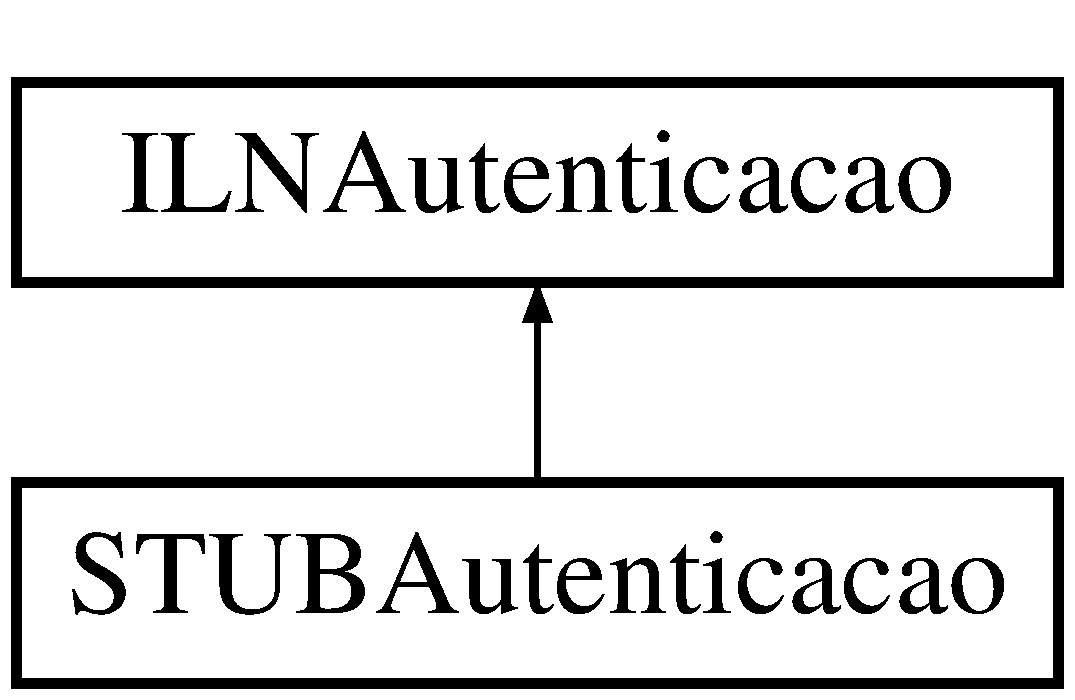
\includegraphics[height=2.000000cm]{classSTUBAutenticacao}
\end{center}
\end{figure}
\subsection*{Public Member Functions}
\begin{DoxyCompactItemize}
\item 
\hyperlink{classResultado}{Resultado} \hyperlink{classSTUBAutenticacao_a4b86dce88ab27b7b8d3fda491690bb18}{autenticar} (const \hyperlink{classApelido}{Apelido} \&, const \hyperlink{classSenha}{Senha} \&)  throw (runtime\+\_\+error)
\end{DoxyCompactItemize}
\subsection*{Static Public Attributes}
\begin{DoxyCompactItemize}
\item 
\mbox{\Hypertarget{classSTUBAutenticacao_a1ef623ead776d172cdcf868ceeb54cdf}\label{classSTUBAutenticacao_a1ef623ead776d172cdcf868ceeb54cdf}} 
static const string {\bfseries T\+R\+I\+G\+G\+E\+R\+\_\+\+F\+A\+L\+H\+A\+\_\+\+A\+U\+T\+E\+N\+T\+I\+C\+A\+C\+AO} = \char`\"{}malu\char`\"{}
\item 
\mbox{\Hypertarget{classSTUBAutenticacao_a7c598d8ac99b7dfc652bd2c7c617d29f}\label{classSTUBAutenticacao_a7c598d8ac99b7dfc652bd2c7c617d29f}} 
static const string {\bfseries T\+R\+I\+G\+G\+E\+R\+\_\+\+E\+R\+R\+O\+\_\+\+S\+I\+S\+T\+E\+M\+A\+\_\+\+A\+U\+T\+E\+N\+T\+I\+C\+A\+C\+AO} = \char`\"{}cao\char`\"{}
\end{DoxyCompactItemize}


\subsection{Detailed Description}
Classe que representa o S\+T\+UB de autenticação. 

\subsection{Member Function Documentation}
\mbox{\Hypertarget{classSTUBAutenticacao_a4b86dce88ab27b7b8d3fda491690bb18}\label{classSTUBAutenticacao_a4b86dce88ab27b7b8d3fda491690bb18}} 
\index{S\+T\+U\+B\+Autenticacao@{S\+T\+U\+B\+Autenticacao}!autenticar@{autenticar}}
\index{autenticar@{autenticar}!S\+T\+U\+B\+Autenticacao@{S\+T\+U\+B\+Autenticacao}}
\subsubsection{\texorpdfstring{autenticar()}{autenticar()}}
{\footnotesize\ttfamily \hyperlink{classResultado}{Resultado} S\+T\+U\+B\+Autenticacao\+::autenticar (\begin{DoxyParamCaption}\item[{const \hyperlink{classApelido}{Apelido} \&}]{apelido,  }\item[{const \hyperlink{classSenha}{Senha} \&}]{senha }\end{DoxyParamCaption}) throw  runtime\+\_\+error) \hspace{0.3cm}{\ttfamily [virtual]}}

Método de implementação do S\+T\+UB do cadastro de autenticação 

Implements \hyperlink{classILNAutenticacao}{I\+L\+N\+Autenticacao}.



The documentation for this class was generated from the following files\+:\begin{DoxyCompactItemize}
\item 
stubs.\+h\item 
stubs.\+cpp\end{DoxyCompactItemize}

\hypertarget{classSTUBBuscarlivro}{}\section{S\+T\+U\+B\+Buscarlivro Class Reference}
\label{classSTUBBuscarlivro}\index{S\+T\+U\+B\+Buscarlivro@{S\+T\+U\+B\+Buscarlivro}}


Classe que representa o S\+T\+UB de busca por livros.  




{\ttfamily \#include $<$stubs.\+h$>$}

Inheritance diagram for S\+T\+U\+B\+Buscarlivro\+:\begin{figure}[H]
\begin{center}
\leavevmode
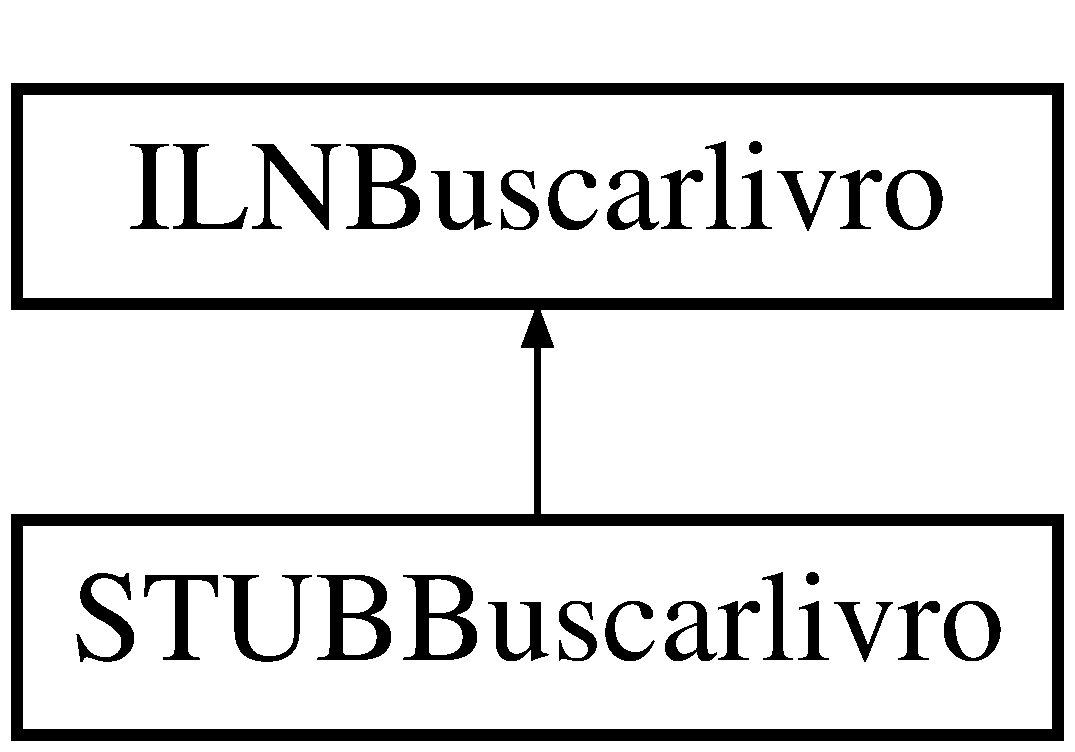
\includegraphics[height=2.000000cm]{classSTUBBuscarlivro}
\end{center}
\end{figure}
\subsection*{Public Member Functions}
\begin{DoxyCompactItemize}
\item 
\hyperlink{classResultado}{Resultado} \hyperlink{classSTUBBuscarlivro_a1c3d0080a08f2e9e7bc57454497b3eca}{buscarlivro} (\hyperlink{classTitulo}{Titulo} titulo)  throw (runtime\+\_\+error)
\end{DoxyCompactItemize}
\subsection*{Static Public Attributes}
\begin{DoxyCompactItemize}
\item 
\mbox{\Hypertarget{classSTUBBuscarlivro_acd3cf870633a937703102409213a4f63}\label{classSTUBBuscarlivro_acd3cf870633a937703102409213a4f63}} 
static const string {\bfseries T\+R\+I\+G\+G\+E\+R\+\_\+\+F\+A\+L\+H\+A\+\_\+\+B\+U\+S\+C\+A\+R\+\_\+\+L\+I\+V\+RO} = \char`\"{}forrest\char`\"{}
\item 
\mbox{\Hypertarget{classSTUBBuscarlivro_a6f8d3e3d50b130baeea5945e874b3bf3}\label{classSTUBBuscarlivro_a6f8d3e3d50b130baeea5945e874b3bf3}} 
static const string {\bfseries T\+R\+I\+G\+G\+E\+R\+\_\+\+E\+R\+R\+O\+\_\+\+S\+I\+S\+T\+E\+M\+A\+\_\+\+B\+U\+S\+C\+A\+R\+\_\+\+L\+I\+V\+RO} = \char`\"{}gump\char`\"{}
\item 
\mbox{\Hypertarget{classSTUBBuscarlivro_a45efb21c64109d5b6ac6a289c061d751}\label{classSTUBBuscarlivro_a45efb21c64109d5b6ac6a289c061d751}} 
static const string {\bfseries L\+I\+V\+R\+O\+\_\+\+C\+A\+D\+A\+S\+T\+R\+A\+DO} = \char`\"{}Lobinho\char`\"{}
\end{DoxyCompactItemize}


\subsection{Detailed Description}
Classe que representa o S\+T\+UB de busca por livros. 

\subsection{Member Function Documentation}
\mbox{\Hypertarget{classSTUBBuscarlivro_a1c3d0080a08f2e9e7bc57454497b3eca}\label{classSTUBBuscarlivro_a1c3d0080a08f2e9e7bc57454497b3eca}} 
\index{S\+T\+U\+B\+Buscarlivro@{S\+T\+U\+B\+Buscarlivro}!buscarlivro@{buscarlivro}}
\index{buscarlivro@{buscarlivro}!S\+T\+U\+B\+Buscarlivro@{S\+T\+U\+B\+Buscarlivro}}
\subsubsection{\texorpdfstring{buscarlivro()}{buscarlivro()}}
{\footnotesize\ttfamily \hyperlink{classResultado}{Resultado} S\+T\+U\+B\+Buscarlivro\+::buscarlivro (\begin{DoxyParamCaption}\item[{\hyperlink{classTitulo}{Titulo}}]{titulo }\end{DoxyParamCaption}) throw  runtime\+\_\+error) \hspace{0.3cm}{\ttfamily [virtual]}}

Método de implementação do S\+T\+UB da busca de livros 

Implements \hyperlink{classILNBuscarlivro}{I\+L\+N\+Buscarlivro}.



The documentation for this class was generated from the following files\+:\begin{DoxyCompactItemize}
\item 
stubs.\+h\item 
stubs.\+cpp\end{DoxyCompactItemize}

\hypertarget{classSTUBBuscarusuario}{}\section{S\+T\+U\+B\+Buscarusuario Class Reference}
\label{classSTUBBuscarusuario}\index{S\+T\+U\+B\+Buscarusuario@{S\+T\+U\+B\+Buscarusuario}}


Classe que representa o S\+T\+UB de busca por usuários.  




{\ttfamily \#include $<$stubs.\+h$>$}

Inheritance diagram for S\+T\+U\+B\+Buscarusuario\+:\begin{figure}[H]
\begin{center}
\leavevmode
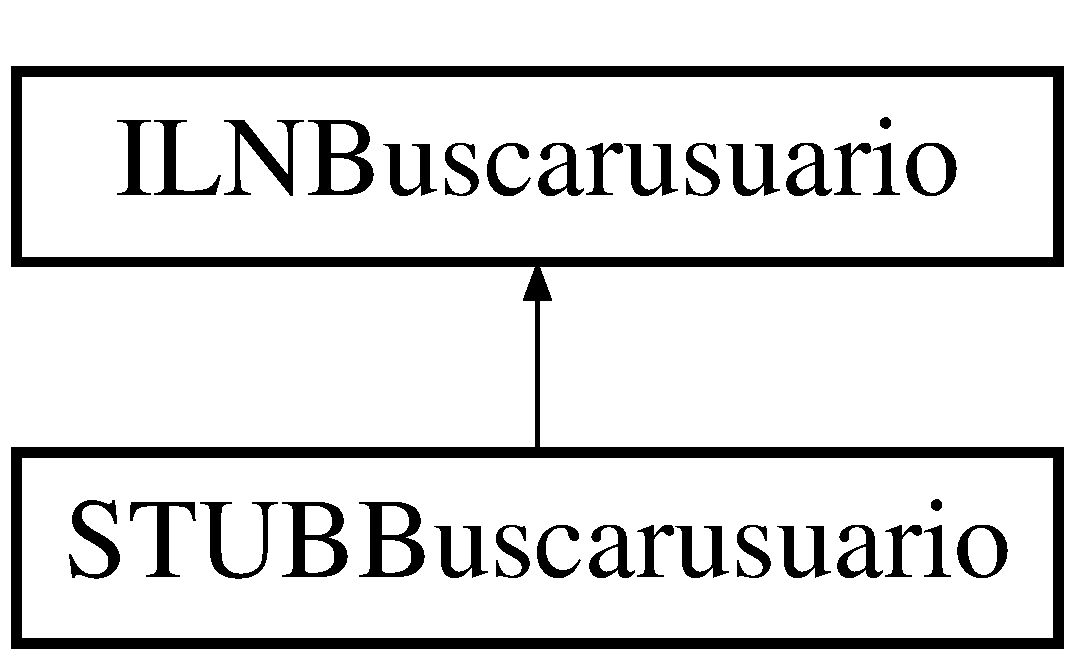
\includegraphics[height=2.000000cm]{classSTUBBuscarusuario}
\end{center}
\end{figure}
\subsection*{Public Member Functions}
\begin{DoxyCompactItemize}
\item 
\hyperlink{classResultado}{Resultado} \hyperlink{classSTUBBuscarusuario_a560dc5bf8f0a64163502ab496046c985}{buscarusuario} (\hyperlink{classApelido}{Apelido} apelido)  throw (runtime\+\_\+error)
\end{DoxyCompactItemize}
\subsection*{Static Public Attributes}
\begin{DoxyCompactItemize}
\item 
\mbox{\Hypertarget{classSTUBBuscarusuario_a47c8339e9b3576007afa98a8be1e5ec8}\label{classSTUBBuscarusuario_a47c8339e9b3576007afa98a8be1e5ec8}} 
static const string {\bfseries T\+R\+I\+G\+G\+E\+R\+\_\+\+F\+A\+L\+H\+A\+\_\+\+B\+U\+S\+C\+A\+R\+\_\+\+U\+S\+U\+A\+R\+IO} = \char`\"{}luca\char`\"{}
\item 
\mbox{\Hypertarget{classSTUBBuscarusuario_a7e000fa79422cdd12702bd3e7463d129}\label{classSTUBBuscarusuario_a7e000fa79422cdd12702bd3e7463d129}} 
static const string {\bfseries T\+R\+I\+G\+G\+E\+R\+\_\+\+E\+R\+R\+O\+\_\+\+S\+I\+S\+T\+E\+M\+A\+\_\+\+B\+U\+S\+C\+A\+R\+\_\+\+U\+S\+U\+A\+R\+IO} = \char`\"{}caio\char`\"{}
\item 
\mbox{\Hypertarget{classSTUBBuscarusuario_ac1b3a0f4334da571cb8cb89b2ad57643}\label{classSTUBBuscarusuario_ac1b3a0f4334da571cb8cb89b2ad57643}} 
static const string {\bfseries U\+S\+U\+A\+R\+I\+O\+\_\+\+C\+A\+D\+A\+S\+T\+R\+A\+DO} = \char`\"{}jon\char`\"{}
\end{DoxyCompactItemize}


\subsection{Detailed Description}
Classe que representa o S\+T\+UB de busca por usuários. 

\subsection{Member Function Documentation}
\mbox{\Hypertarget{classSTUBBuscarusuario_a560dc5bf8f0a64163502ab496046c985}\label{classSTUBBuscarusuario_a560dc5bf8f0a64163502ab496046c985}} 
\index{S\+T\+U\+B\+Buscarusuario@{S\+T\+U\+B\+Buscarusuario}!buscarusuario@{buscarusuario}}
\index{buscarusuario@{buscarusuario}!S\+T\+U\+B\+Buscarusuario@{S\+T\+U\+B\+Buscarusuario}}
\subsubsection{\texorpdfstring{buscarusuario()}{buscarusuario()}}
{\footnotesize\ttfamily \hyperlink{classResultado}{Resultado} S\+T\+U\+B\+Buscarusuario\+::buscarusuario (\begin{DoxyParamCaption}\item[{\hyperlink{classApelido}{Apelido}}]{apelido }\end{DoxyParamCaption}) throw  runtime\+\_\+error) \hspace{0.3cm}{\ttfamily [virtual]}}

Método de implementação do S\+T\+UB da busca de usuários 

Implements \hyperlink{classILNBuscarusuario}{I\+L\+N\+Buscarusuario}.



The documentation for this class was generated from the following files\+:\begin{DoxyCompactItemize}
\item 
stubs.\+h\item 
stubs.\+cpp\end{DoxyCompactItemize}

\hypertarget{classSTUBCadastro}{}\section{S\+T\+U\+B\+Cadastro Class Reference}
\label{classSTUBCadastro}\index{S\+T\+U\+B\+Cadastro@{S\+T\+U\+B\+Cadastro}}


Classe que representa o S\+T\+UB de cadastro de usuários.  




{\ttfamily \#include $<$stubs.\+h$>$}

Inheritance diagram for S\+T\+U\+B\+Cadastro\+:\begin{figure}[H]
\begin{center}
\leavevmode
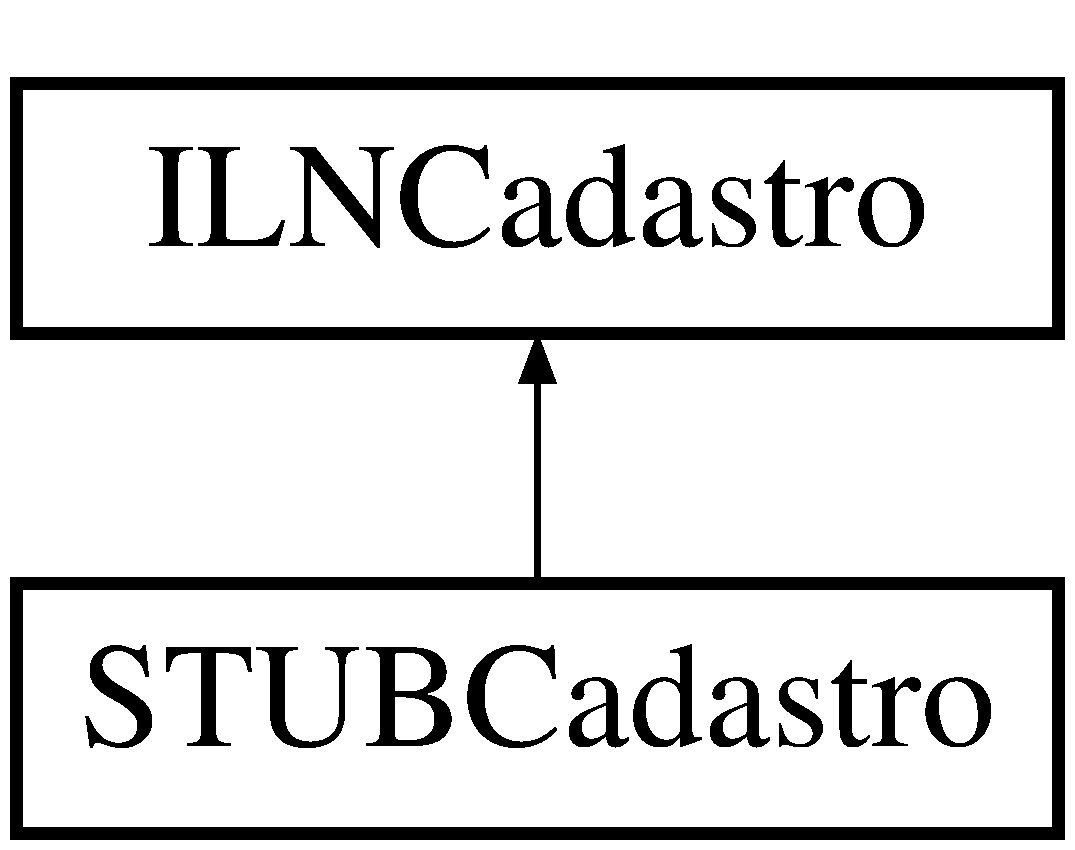
\includegraphics[height=2.000000cm]{classSTUBCadastro}
\end{center}
\end{figure}
\subsection*{Public Member Functions}
\begin{DoxyCompactItemize}
\item 
\hyperlink{classResultado}{Resultado} \hyperlink{classSTUBCadastro_a030d1572eee2691495fc4401c052d99b}{cadastrar} (\hyperlink{classNome}{Nome} nome, \hyperlink{classApelido}{Apelido} apelido, \hyperlink{classSenha}{Senha} senha, \hyperlink{classTelefone}{Telefone} telefone)  throw (runtime\+\_\+error)
\end{DoxyCompactItemize}
\subsection*{Static Public Attributes}
\begin{DoxyCompactItemize}
\item 
\mbox{\Hypertarget{classSTUBCadastro_a4cb2c182b8e8637adff931bd593dfca3}\label{classSTUBCadastro_a4cb2c182b8e8637adff931bd593dfca3}} 
static const string {\bfseries T\+R\+I\+G\+G\+E\+R\+\_\+\+F\+A\+L\+H\+A\+\_\+\+C\+A\+D\+A\+S\+T\+RO} = \char`\"{}Lucas\char`\"{}
\item 
\mbox{\Hypertarget{classSTUBCadastro_aced27b1215db103532d8ec4418e57ffb}\label{classSTUBCadastro_aced27b1215db103532d8ec4418e57ffb}} 
static const string {\bfseries T\+R\+I\+G\+G\+E\+R\+\_\+\+E\+R\+R\+O\+\_\+\+S\+I\+S\+T\+E\+M\+A\+\_\+\+C\+A\+D\+A\+S\+T\+RO} = \char`\"{}Caio\char`\"{}
\end{DoxyCompactItemize}


\subsection{Detailed Description}
Classe que representa o S\+T\+UB de cadastro de usuários. 

\subsection{Member Function Documentation}
\mbox{\Hypertarget{classSTUBCadastro_a030d1572eee2691495fc4401c052d99b}\label{classSTUBCadastro_a030d1572eee2691495fc4401c052d99b}} 
\index{S\+T\+U\+B\+Cadastro@{S\+T\+U\+B\+Cadastro}!cadastrar@{cadastrar}}
\index{cadastrar@{cadastrar}!S\+T\+U\+B\+Cadastro@{S\+T\+U\+B\+Cadastro}}
\subsubsection{\texorpdfstring{cadastrar()}{cadastrar()}}
{\footnotesize\ttfamily \hyperlink{classResultado}{Resultado} S\+T\+U\+B\+Cadastro\+::cadastrar (\begin{DoxyParamCaption}\item[{\hyperlink{classNome}{Nome}}]{nome,  }\item[{\hyperlink{classApelido}{Apelido}}]{apelido,  }\item[{\hyperlink{classSenha}{Senha}}]{senha,  }\item[{\hyperlink{classTelefone}{Telefone}}]{telefone }\end{DoxyParamCaption}) throw  runtime\+\_\+error) \hspace{0.3cm}{\ttfamily [virtual]}}

Método de implementação do S\+T\+UB do cadastro de usuários 

Implements \hyperlink{classILNCadastro}{I\+L\+N\+Cadastro}.



The documentation for this class was generated from the following files\+:\begin{DoxyCompactItemize}
\item 
stubs.\+h\item 
stubs.\+cpp\end{DoxyCompactItemize}

\hypertarget{classSTUBCadastrolivro}{}\section{S\+T\+U\+B\+Cadastrolivro Class Reference}
\label{classSTUBCadastrolivro}\index{S\+T\+U\+B\+Cadastrolivro@{S\+T\+U\+B\+Cadastrolivro}}


Classe que representa o S\+T\+UB de cadastro de livros.  




{\ttfamily \#include $<$stubs.\+h$>$}

Inheritance diagram for S\+T\+U\+B\+Cadastrolivro\+:\begin{figure}[H]
\begin{center}
\leavevmode
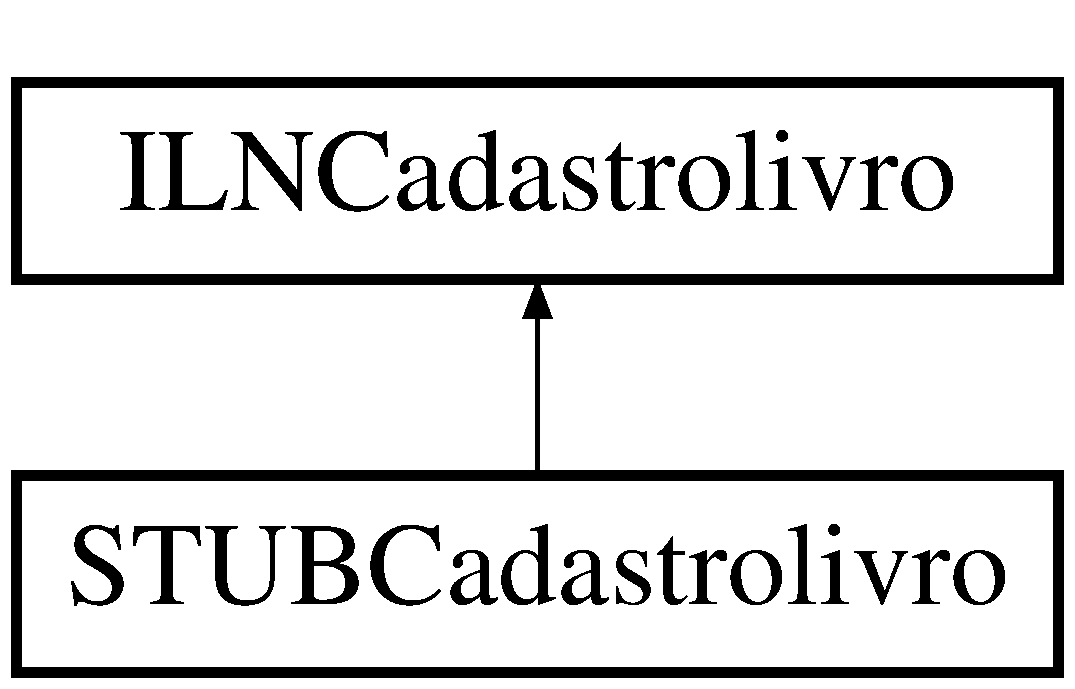
\includegraphics[height=2.000000cm]{classSTUBCadastrolivro}
\end{center}
\end{figure}
\subsection*{Public Member Functions}
\begin{DoxyCompactItemize}
\item 
\hyperlink{classResultado}{Resultado} \hyperlink{classSTUBCadastrolivro_ae0ef9f6f0a4ea7c397285b4a609bf07b}{cadastrarlivro} (const \hyperlink{classTitulo}{Titulo} \&, const \hyperlink{classNome}{Nome} \&, const \hyperlink{classData}{Data} \&, const \hyperlink{classCodigo}{Codigo} \&, const \hyperlink{classGenero}{Genero} \&)  throw (runtime\+\_\+error)
\end{DoxyCompactItemize}
\subsection*{Static Public Attributes}
\begin{DoxyCompactItemize}
\item 
\mbox{\Hypertarget{classSTUBCadastrolivro_a2623ead55b1b8332c8c69291d5e1b49d}\label{classSTUBCadastrolivro_a2623ead55b1b8332c8c69291d5e1b49d}} 
static const string {\bfseries T\+R\+I\+G\+G\+E\+R\+\_\+\+F\+A\+L\+H\+A\+\_\+\+C\+A\+D\+A\+S\+T\+R\+O\+\_\+\+L\+I\+V\+RO} = \char`\"{}12/12/12\char`\"{}
\item 
\mbox{\Hypertarget{classSTUBCadastrolivro_aa4536f549272d3878dc791211779353e}\label{classSTUBCadastrolivro_aa4536f549272d3878dc791211779353e}} 
static const string {\bfseries T\+R\+I\+G\+G\+E\+R\+\_\+\+E\+R\+R\+O\+\_\+\+S\+I\+S\+T\+E\+M\+A\+\_\+\+C\+A\+D\+A\+S\+T\+R\+O\+\_\+\+L\+I\+V\+RO} = \char`\"{}12/11/12\char`\"{}
\end{DoxyCompactItemize}


\subsection{Detailed Description}
Classe que representa o S\+T\+UB de cadastro de livros. 

\subsection{Member Function Documentation}
\mbox{\Hypertarget{classSTUBCadastrolivro_ae0ef9f6f0a4ea7c397285b4a609bf07b}\label{classSTUBCadastrolivro_ae0ef9f6f0a4ea7c397285b4a609bf07b}} 
\index{S\+T\+U\+B\+Cadastrolivro@{S\+T\+U\+B\+Cadastrolivro}!cadastrarlivro@{cadastrarlivro}}
\index{cadastrarlivro@{cadastrarlivro}!S\+T\+U\+B\+Cadastrolivro@{S\+T\+U\+B\+Cadastrolivro}}
\subsubsection{\texorpdfstring{cadastrarlivro()}{cadastrarlivro()}}
{\footnotesize\ttfamily \hyperlink{classResultado}{Resultado} S\+T\+U\+B\+Cadastrolivro\+::cadastrarlivro (\begin{DoxyParamCaption}\item[{const \hyperlink{classTitulo}{Titulo} \&}]{titulo,  }\item[{const \hyperlink{classNome}{Nome} \&}]{autor,  }\item[{const \hyperlink{classData}{Data} \&}]{data,  }\item[{const \hyperlink{classCodigo}{Codigo} \&}]{codigo,  }\item[{const \hyperlink{classGenero}{Genero} \&}]{genero }\end{DoxyParamCaption}) throw  runtime\+\_\+error) \hspace{0.3cm}{\ttfamily [virtual]}}

Método de implementação do S\+T\+UB do cadastro de livros 

Implements \hyperlink{classILNCadastrolivro}{I\+L\+N\+Cadastrolivro}.



The documentation for this class was generated from the following files\+:\begin{DoxyCompactItemize}
\item 
stubs.\+h\item 
stubs.\+cpp\end{DoxyCompactItemize}

\hypertarget{classSTUBComandosusuarioautenticado}{}\section{S\+T\+U\+B\+Comandosusuarioautenticado Class Reference}
\label{classSTUBComandosusuarioautenticado}\index{S\+T\+U\+B\+Comandosusuarioautenticado@{S\+T\+U\+B\+Comandosusuarioautenticado}}


Classe que representa o S\+T\+UB de comandos de um usuário autenticado.  




{\ttfamily \#include $<$stubs.\+h$>$}

Inheritance diagram for S\+T\+U\+B\+Comandosusuarioautenticado\+:\begin{figure}[H]
\begin{center}
\leavevmode
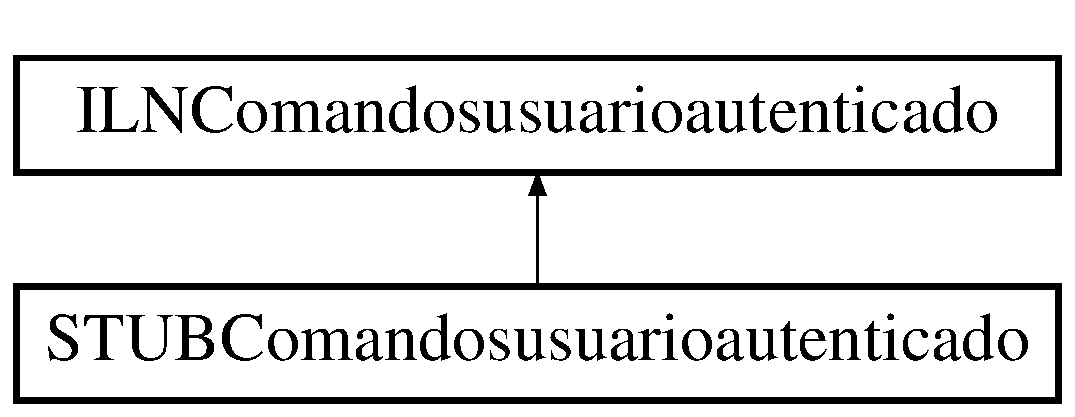
\includegraphics[height=2.000000cm]{classSTUBComandosusuarioautenticado}
\end{center}
\end{figure}
\subsection*{Public Member Functions}
\begin{DoxyCompactItemize}
\item 
\hyperlink{classResultado}{Resultado} \hyperlink{classSTUBComandosusuarioautenticado_ac9e1818a8953c75e8c608f2eac526d4d}{incluir} (const \hyperlink{classTitulo}{Titulo} \&, const \hyperlink{classNome}{Nome} \&, const \hyperlink{classData}{Data} \&, const \hyperlink{classCodigo}{Codigo} \&, const \hyperlink{classGenero}{Genero} \&)  throw (runtime\+\_\+error)
\item 
\hyperlink{classResultado}{Resultado} \hyperlink{classSTUBComandosusuarioautenticado_a80c1a29ca48ebb60f6ba0d417946d595}{remover} (const \hyperlink{classTitulo}{Titulo} \&)  throw (runtime\+\_\+error)
\item 
\hyperlink{classResultado}{Resultado} \hyperlink{classSTUBComandosusuarioautenticado_a39e1508359209fe795a91817f0c96e20}{registrarresenha} (const \hyperlink{classNome}{Nome} \&, const \hyperlink{classTitulo}{Titulo} \&, const \hyperlink{classTexto}{Texto} \&)  throw (runtime\+\_\+error)
\item 
\hyperlink{classResultado}{Resultado} \hyperlink{classSTUBComandosusuarioautenticado_a435e243be205e8898efb085ff40aedc2}{trocarlivro} (const \hyperlink{classTitulo}{Titulo} \&)  throw (runtime\+\_\+error)
\item 
\hyperlink{classResultado}{Resultado} \hyperlink{classSTUBComandosusuarioautenticado_a12f684d2240412050e6eee54ebdd1a57}{buscarlivro} (const \hyperlink{classTitulo}{Titulo} \&)  throw (runtime\+\_\+error)
\item 
\hyperlink{classResultado}{Resultado} \hyperlink{classSTUBComandosusuarioautenticado_ad156d9cd3554e120bc8fff5916955465}{buscarusuario} (const \hyperlink{classApelido}{Apelido} \&)  throw (runtime\+\_\+error)
\end{DoxyCompactItemize}
\subsection*{Static Public Attributes}
\begin{DoxyCompactItemize}
\item 
\mbox{\Hypertarget{classSTUBComandosusuarioautenticado_a6130917026c71c1c20d2aee41ab916a8}\label{classSTUBComandosusuarioautenticado_a6130917026c71c1c20d2aee41ab916a8}} 
static const string {\bfseries T\+R\+I\+G\+G\+E\+R\+\_\+\+F\+A\+L\+H\+A\+\_\+\+C\+A\+D\+A\+S\+T\+R\+O\+\_\+\+L\+I\+V\+RO} = \char`\"{}forrest\char`\"{}
\item 
\mbox{\Hypertarget{classSTUBComandosusuarioautenticado_a07ca908a055324beeb90eab1f3926933}\label{classSTUBComandosusuarioautenticado_a07ca908a055324beeb90eab1f3926933}} 
static const string {\bfseries T\+R\+I\+G\+G\+E\+R\+\_\+\+E\+R\+R\+O\+\_\+\+S\+I\+S\+T\+E\+M\+A\+\_\+\+C\+A\+D\+A\+S\+T\+R\+O\+\_\+\+L\+I\+V\+RO} = \char`\"{}gump\char`\"{}
\item 
\mbox{\Hypertarget{classSTUBComandosusuarioautenticado_a5b1058157df116b390a06c1f802b8c3b}\label{classSTUBComandosusuarioautenticado_a5b1058157df116b390a06c1f802b8c3b}} 
static const string {\bfseries T\+R\+I\+G\+G\+E\+R\+\_\+\+F\+A\+L\+H\+A\+\_\+\+R\+E\+G\+I\+S\+T\+R\+O\+\_\+\+R\+E\+S\+E\+N\+HA} = \char`\"{}B\+A\+N\+A\+NA\char`\"{}
\item 
\mbox{\Hypertarget{classSTUBComandosusuarioautenticado_a9f46bca32f1eb4d9efdf336f63c40397}\label{classSTUBComandosusuarioautenticado_a9f46bca32f1eb4d9efdf336f63c40397}} 
static const string {\bfseries T\+R\+I\+G\+G\+E\+R\+\_\+\+E\+R\+R\+O\+\_\+\+S\+I\+S\+T\+E\+M\+A\+\_\+\+R\+E\+G\+I\+S\+T\+R\+O\+\_\+\+R\+E\+S\+E\+N\+HA} = \char`\"{}L\+A\+R\+A\+N\+JA\char`\"{}
\item 
\mbox{\Hypertarget{classSTUBComandosusuarioautenticado_aaf54abf3405c0feca3ebc1130ed2d9ae}\label{classSTUBComandosusuarioautenticado_aaf54abf3405c0feca3ebc1130ed2d9ae}} 
static const string {\bfseries T\+R\+I\+G\+G\+E\+R\+\_\+\+F\+A\+L\+H\+A\+\_\+\+B\+U\+S\+C\+A\+R\+\_\+\+U\+S\+U\+A\+R\+IO} = \char`\"{}luca\char`\"{}
\item 
\mbox{\Hypertarget{classSTUBComandosusuarioautenticado_ab9d312722af5596334113f2afea9646d}\label{classSTUBComandosusuarioautenticado_ab9d312722af5596334113f2afea9646d}} 
static const string {\bfseries T\+R\+I\+G\+G\+E\+R\+\_\+\+E\+R\+R\+O\+\_\+\+S\+I\+S\+T\+E\+M\+A\+\_\+\+B\+U\+S\+C\+A\+R\+\_\+\+U\+S\+U\+A\+R\+IO} = \char`\"{}caio\char`\"{}
\item 
\mbox{\Hypertarget{classSTUBComandosusuarioautenticado_a55a441d1b1a4c579d028f23eb9fe6611}\label{classSTUBComandosusuarioautenticado_a55a441d1b1a4c579d028f23eb9fe6611}} 
static const string {\bfseries T\+R\+I\+G\+G\+E\+R\+\_\+\+F\+A\+L\+H\+A\+\_\+\+B\+U\+S\+C\+A\+R\+\_\+\+L\+I\+V\+RO} = \char`\"{}forrest\char`\"{}
\item 
\mbox{\Hypertarget{classSTUBComandosusuarioautenticado_a29ead874532d57f9f1b86f8c287f813a}\label{classSTUBComandosusuarioautenticado_a29ead874532d57f9f1b86f8c287f813a}} 
static const string {\bfseries T\+R\+I\+G\+G\+E\+R\+\_\+\+E\+R\+R\+O\+\_\+\+S\+I\+S\+T\+E\+M\+A\+\_\+\+B\+U\+S\+C\+A\+R\+\_\+\+L\+I\+V\+RO} = \char`\"{}gump\char`\"{}
\item 
\mbox{\Hypertarget{classSTUBComandosusuarioautenticado_a6af222cd1eff0bac96ab7194d496c903}\label{classSTUBComandosusuarioautenticado_a6af222cd1eff0bac96ab7194d496c903}} 
static const string {\bfseries T\+R\+I\+G\+G\+E\+R\+\_\+\+F\+A\+L\+H\+A\+\_\+\+T\+R\+O\+C\+A\+R\+\_\+\+L\+I\+V\+RO} = \char`\"{}forrest\char`\"{}
\item 
\mbox{\Hypertarget{classSTUBComandosusuarioautenticado_ada4a785006c657fb829db2b2f764af4d}\label{classSTUBComandosusuarioautenticado_ada4a785006c657fb829db2b2f764af4d}} 
static const string {\bfseries T\+R\+I\+G\+G\+E\+R\+\_\+\+E\+R\+R\+O\+\_\+\+S\+I\+S\+T\+E\+M\+A\+\_\+\+T\+R\+O\+C\+A\+R\+\_\+\+L\+I\+V\+RO} = \char`\"{}gump\char`\"{}
\item 
\mbox{\Hypertarget{classSTUBComandosusuarioautenticado_a5488361abe4431ae3f37b57f45d11f1f}\label{classSTUBComandosusuarioautenticado_a5488361abe4431ae3f37b57f45d11f1f}} 
static const string {\bfseries L\+I\+V\+R\+O\+\_\+\+D\+I\+S\+P\+O\+N\+I\+V\+E\+L\+\_\+\+T\+R\+O\+CA} = \char`\"{}Lobinho\char`\"{}
\item 
\mbox{\Hypertarget{classSTUBComandosusuarioautenticado_a6f5b109074186321b63b1bbb55be8b88}\label{classSTUBComandosusuarioautenticado_a6f5b109074186321b63b1bbb55be8b88}} 
static const string {\bfseries L\+I\+V\+R\+O\+\_\+\+C\+A\+D\+A\+S\+T\+R\+A\+DO} = \char`\"{}Lobinho\char`\"{}
\item 
\mbox{\Hypertarget{classSTUBComandosusuarioautenticado_a3fae6f1d9ef8d902f72f6bcd9044a3c3}\label{classSTUBComandosusuarioautenticado_a3fae6f1d9ef8d902f72f6bcd9044a3c3}} 
static const string {\bfseries U\+S\+U\+A\+R\+I\+O\+\_\+\+C\+A\+D\+A\+S\+T\+R\+A\+DO} = \char`\"{}jon\char`\"{}
\end{DoxyCompactItemize}


\subsection{Detailed Description}
Classe que representa o S\+T\+UB de comandos de um usuário autenticado. 

\subsection{Member Function Documentation}
\mbox{\Hypertarget{classSTUBComandosusuarioautenticado_a12f684d2240412050e6eee54ebdd1a57}\label{classSTUBComandosusuarioautenticado_a12f684d2240412050e6eee54ebdd1a57}} 
\index{S\+T\+U\+B\+Comandosusuarioautenticado@{S\+T\+U\+B\+Comandosusuarioautenticado}!buscarlivro@{buscarlivro}}
\index{buscarlivro@{buscarlivro}!S\+T\+U\+B\+Comandosusuarioautenticado@{S\+T\+U\+B\+Comandosusuarioautenticado}}
\subsubsection{\texorpdfstring{buscarlivro()}{buscarlivro()}}
{\footnotesize\ttfamily \hyperlink{classResultado}{Resultado} S\+T\+U\+B\+Comandosusuarioautenticado\+::buscarlivro (\begin{DoxyParamCaption}\item[{const \hyperlink{classTitulo}{Titulo} \&}]{titulo }\end{DoxyParamCaption}) throw  runtime\+\_\+error) \hspace{0.3cm}{\ttfamily [virtual]}}

Método de implementação do S\+T\+UB do comando de busca de livros de um usuário autenticado 

Implements \hyperlink{classILNComandosusuarioautenticado}{I\+L\+N\+Comandosusuarioautenticado}.

\mbox{\Hypertarget{classSTUBComandosusuarioautenticado_ad156d9cd3554e120bc8fff5916955465}\label{classSTUBComandosusuarioautenticado_ad156d9cd3554e120bc8fff5916955465}} 
\index{S\+T\+U\+B\+Comandosusuarioautenticado@{S\+T\+U\+B\+Comandosusuarioautenticado}!buscarusuario@{buscarusuario}}
\index{buscarusuario@{buscarusuario}!S\+T\+U\+B\+Comandosusuarioautenticado@{S\+T\+U\+B\+Comandosusuarioautenticado}}
\subsubsection{\texorpdfstring{buscarusuario()}{buscarusuario()}}
{\footnotesize\ttfamily \hyperlink{classResultado}{Resultado} S\+T\+U\+B\+Comandosusuarioautenticado\+::buscarusuario (\begin{DoxyParamCaption}\item[{const \hyperlink{classApelido}{Apelido} \&}]{apelido }\end{DoxyParamCaption}) throw  runtime\+\_\+error) \hspace{0.3cm}{\ttfamily [virtual]}}

Método de implementação do S\+T\+UB do comando de busca de usuários de um usuário autenticado 

Implements \hyperlink{classILNComandosusuarioautenticado}{I\+L\+N\+Comandosusuarioautenticado}.

\mbox{\Hypertarget{classSTUBComandosusuarioautenticado_ac9e1818a8953c75e8c608f2eac526d4d}\label{classSTUBComandosusuarioautenticado_ac9e1818a8953c75e8c608f2eac526d4d}} 
\index{S\+T\+U\+B\+Comandosusuarioautenticado@{S\+T\+U\+B\+Comandosusuarioautenticado}!incluir@{incluir}}
\index{incluir@{incluir}!S\+T\+U\+B\+Comandosusuarioautenticado@{S\+T\+U\+B\+Comandosusuarioautenticado}}
\subsubsection{\texorpdfstring{incluir()}{incluir()}}
{\footnotesize\ttfamily \hyperlink{classResultado}{Resultado} S\+T\+U\+B\+Comandosusuarioautenticado\+::incluir (\begin{DoxyParamCaption}\item[{const \hyperlink{classTitulo}{Titulo} \&}]{titulo,  }\item[{const \hyperlink{classNome}{Nome} \&}]{autor,  }\item[{const \hyperlink{classData}{Data} \&}]{data,  }\item[{const \hyperlink{classCodigo}{Codigo} \&}]{codigo,  }\item[{const \hyperlink{classGenero}{Genero} \&}]{genero }\end{DoxyParamCaption}) throw  runtime\+\_\+error) \hspace{0.3cm}{\ttfamily [virtual]}}

Método de implementação do S\+T\+UB do comando de inclusão de um usuário autenticado 

Implements \hyperlink{classILNComandosusuarioautenticado}{I\+L\+N\+Comandosusuarioautenticado}.

\mbox{\Hypertarget{classSTUBComandosusuarioautenticado_a39e1508359209fe795a91817f0c96e20}\label{classSTUBComandosusuarioautenticado_a39e1508359209fe795a91817f0c96e20}} 
\index{S\+T\+U\+B\+Comandosusuarioautenticado@{S\+T\+U\+B\+Comandosusuarioautenticado}!registrarresenha@{registrarresenha}}
\index{registrarresenha@{registrarresenha}!S\+T\+U\+B\+Comandosusuarioautenticado@{S\+T\+U\+B\+Comandosusuarioautenticado}}
\subsubsection{\texorpdfstring{registrarresenha()}{registrarresenha()}}
{\footnotesize\ttfamily \hyperlink{classResultado}{Resultado} S\+T\+U\+B\+Comandosusuarioautenticado\+::registrarresenha (\begin{DoxyParamCaption}\item[{const \hyperlink{classNome}{Nome} \&}]{autor,  }\item[{const \hyperlink{classTitulo}{Titulo} \&}]{titulo,  }\item[{const \hyperlink{classTexto}{Texto} \&}]{texto }\end{DoxyParamCaption}) throw  runtime\+\_\+error) \hspace{0.3cm}{\ttfamily [virtual]}}

Método de implementação do S\+T\+UB do comando de registro de resenhas de um usuário autenticado 

Implements \hyperlink{classILNComandosusuarioautenticado}{I\+L\+N\+Comandosusuarioautenticado}.

\mbox{\Hypertarget{classSTUBComandosusuarioautenticado_a80c1a29ca48ebb60f6ba0d417946d595}\label{classSTUBComandosusuarioautenticado_a80c1a29ca48ebb60f6ba0d417946d595}} 
\index{S\+T\+U\+B\+Comandosusuarioautenticado@{S\+T\+U\+B\+Comandosusuarioautenticado}!remover@{remover}}
\index{remover@{remover}!S\+T\+U\+B\+Comandosusuarioautenticado@{S\+T\+U\+B\+Comandosusuarioautenticado}}
\subsubsection{\texorpdfstring{remover()}{remover()}}
{\footnotesize\ttfamily \hyperlink{classResultado}{Resultado} S\+T\+U\+B\+Comandosusuarioautenticado\+::remover (\begin{DoxyParamCaption}\item[{const \hyperlink{classTitulo}{Titulo} \&}]{titulo }\end{DoxyParamCaption}) throw  runtime\+\_\+error) \hspace{0.3cm}{\ttfamily [virtual]}}

Método de implementação do S\+T\+UB do comando de exclusão de um usuário autenticado 

Implements \hyperlink{classILNComandosusuarioautenticado}{I\+L\+N\+Comandosusuarioautenticado}.

\mbox{\Hypertarget{classSTUBComandosusuarioautenticado_a435e243be205e8898efb085ff40aedc2}\label{classSTUBComandosusuarioautenticado_a435e243be205e8898efb085ff40aedc2}} 
\index{S\+T\+U\+B\+Comandosusuarioautenticado@{S\+T\+U\+B\+Comandosusuarioautenticado}!trocarlivro@{trocarlivro}}
\index{trocarlivro@{trocarlivro}!S\+T\+U\+B\+Comandosusuarioautenticado@{S\+T\+U\+B\+Comandosusuarioautenticado}}
\subsubsection{\texorpdfstring{trocarlivro()}{trocarlivro()}}
{\footnotesize\ttfamily \hyperlink{classResultado}{Resultado} S\+T\+U\+B\+Comandosusuarioautenticado\+::trocarlivro (\begin{DoxyParamCaption}\item[{const \hyperlink{classTitulo}{Titulo} \&}]{titulo }\end{DoxyParamCaption}) throw  runtime\+\_\+error) \hspace{0.3cm}{\ttfamily [virtual]}}

Método de implementação do S\+T\+UB do comando de troca de livros de um usuário autenticado 

Implements \hyperlink{classILNComandosusuarioautenticado}{I\+L\+N\+Comandosusuarioautenticado}.



The documentation for this class was generated from the following files\+:\begin{DoxyCompactItemize}
\item 
stubs.\+h\item 
stubs.\+cpp\end{DoxyCompactItemize}

\hypertarget{classSTUBRegistroresenha}{}\section{S\+T\+U\+B\+Registroresenha Class Reference}
\label{classSTUBRegistroresenha}\index{S\+T\+U\+B\+Registroresenha@{S\+T\+U\+B\+Registroresenha}}


Classe que representa o S\+T\+UB de cadastro de registro de resenhas.  




{\ttfamily \#include $<$stubs.\+h$>$}

Inheritance diagram for S\+T\+U\+B\+Registroresenha\+:\begin{figure}[H]
\begin{center}
\leavevmode
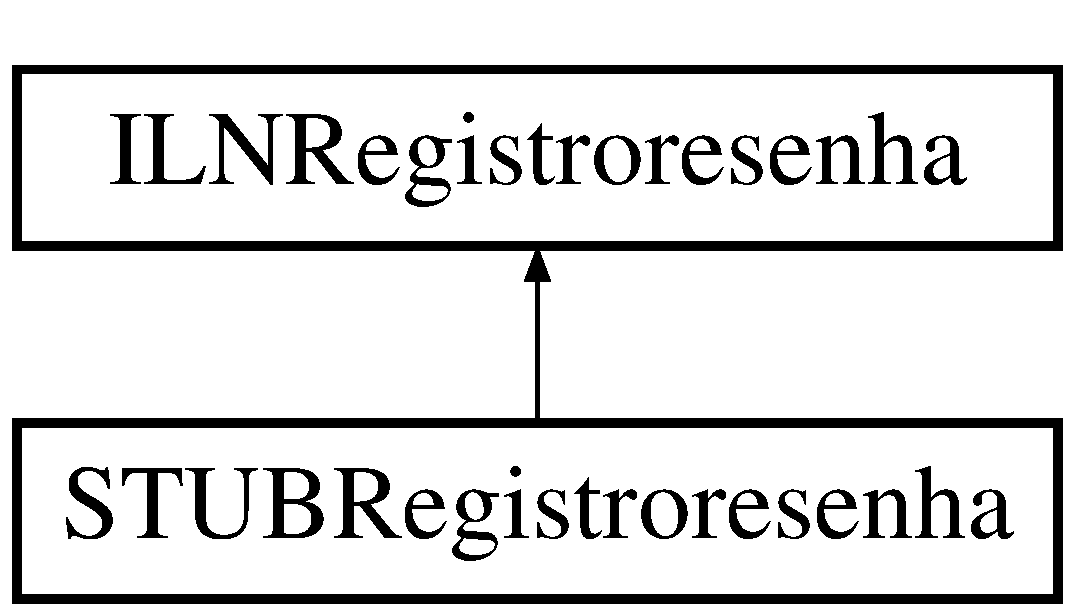
\includegraphics[height=2.000000cm]{classSTUBRegistroresenha}
\end{center}
\end{figure}
\subsection*{Public Member Functions}
\begin{DoxyCompactItemize}
\item 
\hyperlink{classResultado}{Resultado} \hyperlink{classSTUBRegistroresenha_a98762ff953cb017d00a225a0772b6394}{registrarresenha} (const \hyperlink{classNome}{Nome} \&, const \hyperlink{classTitulo}{Titulo} \&, const \hyperlink{classTexto}{Texto} \&)  throw (runtime\+\_\+error)
\end{DoxyCompactItemize}
\subsection*{Static Public Attributes}
\begin{DoxyCompactItemize}
\item 
\mbox{\Hypertarget{classSTUBRegistroresenha_a94328e1c8f7e2e0e6d6483364e2ab68a}\label{classSTUBRegistroresenha_a94328e1c8f7e2e0e6d6483364e2ab68a}} 
static const string {\bfseries T\+R\+I\+G\+G\+E\+R\+\_\+\+F\+A\+L\+H\+A\+\_\+\+R\+E\+G\+I\+S\+T\+R\+O\+\_\+\+R\+E\+S\+E\+N\+HA} = \char`\"{}forrest\char`\"{}
\item 
\mbox{\Hypertarget{classSTUBRegistroresenha_aaa64d45e5b6a55ec5554d3b764d04e74}\label{classSTUBRegistroresenha_aaa64d45e5b6a55ec5554d3b764d04e74}} 
static const string {\bfseries T\+R\+I\+G\+G\+E\+R\+\_\+\+E\+R\+R\+O\+\_\+\+S\+I\+S\+T\+E\+M\+A\+\_\+\+R\+E\+G\+I\+S\+T\+R\+O\+\_\+\+R\+E\+S\+E\+N\+HA} = \char`\"{}gump\char`\"{}
\end{DoxyCompactItemize}


\subsection{Detailed Description}
Classe que representa o S\+T\+UB de cadastro de registro de resenhas. 

\subsection{Member Function Documentation}
\mbox{\Hypertarget{classSTUBRegistroresenha_a98762ff953cb017d00a225a0772b6394}\label{classSTUBRegistroresenha_a98762ff953cb017d00a225a0772b6394}} 
\index{S\+T\+U\+B\+Registroresenha@{S\+T\+U\+B\+Registroresenha}!registrarresenha@{registrarresenha}}
\index{registrarresenha@{registrarresenha}!S\+T\+U\+B\+Registroresenha@{S\+T\+U\+B\+Registroresenha}}
\subsubsection{\texorpdfstring{registrarresenha()}{registrarresenha()}}
{\footnotesize\ttfamily \hyperlink{classResultado}{Resultado} S\+T\+U\+B\+Registroresenha\+::registrarresenha (\begin{DoxyParamCaption}\item[{const \hyperlink{classNome}{Nome} \&}]{autor,  }\item[{const \hyperlink{classTitulo}{Titulo} \&}]{titulo,  }\item[{const \hyperlink{classTexto}{Texto} \&}]{texto }\end{DoxyParamCaption}) throw  runtime\+\_\+error) \hspace{0.3cm}{\ttfamily [virtual]}}

Método de implementação do S\+T\+UB do registro de resenhas 

Implements \hyperlink{classILNRegistroresenha}{I\+L\+N\+Registroresenha}.



The documentation for this class was generated from the following files\+:\begin{DoxyCompactItemize}
\item 
stubs.\+h\item 
stubs.\+cpp\end{DoxyCompactItemize}

\hypertarget{classSTUBTrocarlivro}{}\section{S\+T\+U\+B\+Trocarlivro Class Reference}
\label{classSTUBTrocarlivro}\index{S\+T\+U\+B\+Trocarlivro@{S\+T\+U\+B\+Trocarlivro}}


Classe que representa o S\+T\+UB de troca de livros.  




{\ttfamily \#include $<$stubs.\+h$>$}

Inheritance diagram for S\+T\+U\+B\+Trocarlivro\+:\begin{figure}[H]
\begin{center}
\leavevmode
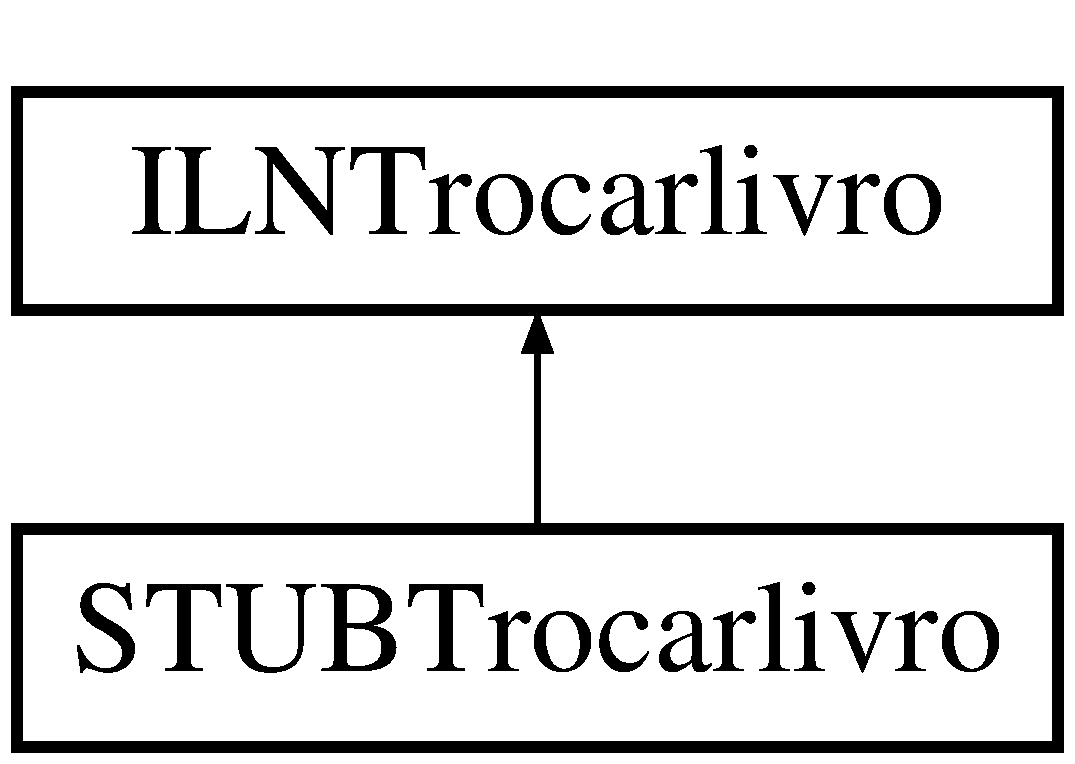
\includegraphics[height=2.000000cm]{classSTUBTrocarlivro}
\end{center}
\end{figure}
\subsection*{Public Member Functions}
\begin{DoxyCompactItemize}
\item 
\hyperlink{classResultado}{Resultado} \hyperlink{classSTUBTrocarlivro_ac94fcf8594839d0edff8f2c9ab556d21}{trocarlivro} (const \hyperlink{classTitulo}{Titulo} \&)  throw (runtime\+\_\+error)
\end{DoxyCompactItemize}
\subsection*{Static Public Attributes}
\begin{DoxyCompactItemize}
\item 
\mbox{\Hypertarget{classSTUBTrocarlivro_a6971aeacf6543cbea47bb134aa71a396}\label{classSTUBTrocarlivro_a6971aeacf6543cbea47bb134aa71a396}} 
static const string {\bfseries T\+R\+I\+G\+G\+E\+R\+\_\+\+F\+A\+L\+H\+A\+\_\+\+T\+R\+O\+C\+A\+R\+\_\+\+L\+I\+V\+RO} = \char`\"{}forrest\char`\"{}
\item 
\mbox{\Hypertarget{classSTUBTrocarlivro_a84a662aa66292900dd8a3eb176653516}\label{classSTUBTrocarlivro_a84a662aa66292900dd8a3eb176653516}} 
static const string {\bfseries T\+R\+I\+G\+G\+E\+R\+\_\+\+E\+R\+R\+O\+\_\+\+S\+I\+S\+T\+E\+M\+A\+\_\+\+T\+R\+O\+C\+A\+R\+\_\+\+L\+I\+V\+RO} = \char`\"{}gump\char`\"{}
\item 
\mbox{\Hypertarget{classSTUBTrocarlivro_a8052c570d33fcb70e9ec015515deb5fd}\label{classSTUBTrocarlivro_a8052c570d33fcb70e9ec015515deb5fd}} 
static const string {\bfseries L\+I\+V\+R\+O\+\_\+\+D\+I\+S\+P\+O\+N\+I\+V\+E\+L\+\_\+\+T\+R\+O\+CA} = \char`\"{}Lobinho\char`\"{}
\end{DoxyCompactItemize}


\subsection{Detailed Description}
Classe que representa o S\+T\+UB de troca de livros. 

\subsection{Member Function Documentation}
\mbox{\Hypertarget{classSTUBTrocarlivro_ac94fcf8594839d0edff8f2c9ab556d21}\label{classSTUBTrocarlivro_ac94fcf8594839d0edff8f2c9ab556d21}} 
\index{S\+T\+U\+B\+Trocarlivro@{S\+T\+U\+B\+Trocarlivro}!trocarlivro@{trocarlivro}}
\index{trocarlivro@{trocarlivro}!S\+T\+U\+B\+Trocarlivro@{S\+T\+U\+B\+Trocarlivro}}
\subsubsection{\texorpdfstring{trocarlivro()}{trocarlivro()}}
{\footnotesize\ttfamily \hyperlink{classResultado}{Resultado} S\+T\+U\+B\+Trocarlivro\+::trocarlivro (\begin{DoxyParamCaption}\item[{const \hyperlink{classTitulo}{Titulo} \&}]{titulo }\end{DoxyParamCaption}) throw  runtime\+\_\+error) \hspace{0.3cm}{\ttfamily [virtual]}}

Método de implementação do S\+T\+UB da troca de livros 

Implements \hyperlink{classILNTrocarlivro}{I\+L\+N\+Trocarlivro}.



The documentation for this class was generated from the following files\+:\begin{DoxyCompactItemize}
\item 
stubs.\+h\item 
stubs.\+cpp\end{DoxyCompactItemize}

\hypertarget{classTelefone}{}\section{Telefone Class Reference}
\label{classTelefone}\index{Telefone@{Telefone}}
\subsection*{Public Member Functions}
\begin{DoxyCompactItemize}
\item 
\mbox{\Hypertarget{classTelefone_a79516b37434ff927bd2a9bd66080a36d}\label{classTelefone_a79516b37434ff927bd2a9bd66080a36d}} 
void {\bfseries set\+Telefone} (string)  throw (invalid\+\_\+argument)
\item 
\mbox{\Hypertarget{classTelefone_a64d1e99657fde65bb698ddcd56e7eb04}\label{classTelefone_a64d1e99657fde65bb698ddcd56e7eb04}} 
string {\bfseries get\+Telefone} () const
\end{DoxyCompactItemize}


The documentation for this class was generated from the following files\+:\begin{DoxyCompactItemize}
\item 
dominios.\+h\item 
dominios.\+cpp\end{DoxyCompactItemize}

\hypertarget{classTexto}{}\section{Texto Class Reference}
\label{classTexto}\index{Texto@{Texto}}
\subsection*{Public Member Functions}
\begin{DoxyCompactItemize}
\item 
\mbox{\Hypertarget{classTexto_a2757e0409bd76bb77c8eb6ecb09cc69d}\label{classTexto_a2757e0409bd76bb77c8eb6ecb09cc69d}} 
void {\bfseries set\+Texto} (string)  throw (invalid\+\_\+argument)
\item 
\mbox{\Hypertarget{classTexto_a69463b543f36eaf86076ef48c896987f}\label{classTexto_a69463b543f36eaf86076ef48c896987f}} 
string {\bfseries get\+Texto} () const
\end{DoxyCompactItemize}


The documentation for this class was generated from the following files\+:\begin{DoxyCompactItemize}
\item 
dominios.\+h\item 
dominios.\+cpp\end{DoxyCompactItemize}

\hypertarget{classTitulo}{}\section{Titulo Class Reference}
\label{classTitulo}\index{Titulo@{Titulo}}
\subsection*{Public Member Functions}
\begin{DoxyCompactItemize}
\item 
\mbox{\Hypertarget{classTitulo_ac4b3e70d24f498a9085ae9d01d51ef12}\label{classTitulo_ac4b3e70d24f498a9085ae9d01d51ef12}} 
void {\bfseries set\+Titulo} (string)  throw (invalid\+\_\+argument)
\item 
\mbox{\Hypertarget{classTitulo_ad13d7166263fe5b8053532a820165390}\label{classTitulo_ad13d7166263fe5b8053532a820165390}} 
string {\bfseries get\+Titulo} () const
\end{DoxyCompactItemize}


The documentation for this class was generated from the following files\+:\begin{DoxyCompactItemize}
\item 
dominios.\+h\item 
dominios.\+cpp\end{DoxyCompactItemize}

\hypertarget{classTUApelido}{}\section{T\+U\+Apelido Class Reference}
\label{classTUApelido}\index{T\+U\+Apelido@{T\+U\+Apelido}}
\subsection*{Public Member Functions}
\begin{DoxyCompactItemize}
\item 
\mbox{\Hypertarget{classTUApelido_ab5aabaa60fd00030d047ef8bf6c55fec}\label{classTUApelido_ab5aabaa60fd00030d047ef8bf6c55fec}} 
int {\bfseries run} ()
\end{DoxyCompactItemize}
\subsection*{Static Public Attributes}
\begin{DoxyCompactItemize}
\item 
\mbox{\Hypertarget{classTUApelido_aa100f19a4867e7bf07c49161bb2efef0}\label{classTUApelido_aa100f19a4867e7bf07c49161bb2efef0}} 
static const int {\bfseries S\+U\+C\+E\+S\+SO} = 0
\item 
\mbox{\Hypertarget{classTUApelido_afdc614cde9b44f65a445dbaf41142698}\label{classTUApelido_afdc614cde9b44f65a445dbaf41142698}} 
static const int {\bfseries F\+A\+L\+HA} = -\/1
\end{DoxyCompactItemize}


The documentation for this class was generated from the following files\+:\begin{DoxyCompactItemize}
\item 
T\+Udominios.\+h\item 
T\+Udominios.\+cpp\end{DoxyCompactItemize}

\hypertarget{classTUCodigo}{}\section{T\+U\+Codigo Class Reference}
\label{classTUCodigo}\index{T\+U\+Codigo@{T\+U\+Codigo}}
\subsection*{Public Member Functions}
\begin{DoxyCompactItemize}
\item 
\mbox{\Hypertarget{classTUCodigo_a4e6994bcde0011cdf0b0bb7a2c4d94d9}\label{classTUCodigo_a4e6994bcde0011cdf0b0bb7a2c4d94d9}} 
int {\bfseries run} ()
\end{DoxyCompactItemize}
\subsection*{Static Public Attributes}
\begin{DoxyCompactItemize}
\item 
\mbox{\Hypertarget{classTUCodigo_ae74fd939ebced94047b47878406f53d1}\label{classTUCodigo_ae74fd939ebced94047b47878406f53d1}} 
static const int {\bfseries S\+U\+C\+E\+S\+SO} = 0
\item 
\mbox{\Hypertarget{classTUCodigo_abff6dd7b04006df40462c76f8b769123}\label{classTUCodigo_abff6dd7b04006df40462c76f8b769123}} 
static const int {\bfseries F\+A\+L\+HA} = -\/1
\end{DoxyCompactItemize}


The documentation for this class was generated from the following files\+:\begin{DoxyCompactItemize}
\item 
T\+Udominios.\+h\item 
T\+Udominios.\+cpp\end{DoxyCompactItemize}

\hypertarget{classTUData}{}\section{T\+U\+Data Class Reference}
\label{classTUData}\index{T\+U\+Data@{T\+U\+Data}}
\subsection*{Public Member Functions}
\begin{DoxyCompactItemize}
\item 
\mbox{\Hypertarget{classTUData_a4fd95b821fa6d55bdc82be6f3a3cbef2}\label{classTUData_a4fd95b821fa6d55bdc82be6f3a3cbef2}} 
int {\bfseries run} ()
\end{DoxyCompactItemize}
\subsection*{Static Public Attributes}
\begin{DoxyCompactItemize}
\item 
\mbox{\Hypertarget{classTUData_a59be2c38007b733030111a5aadfb4517}\label{classTUData_a59be2c38007b733030111a5aadfb4517}} 
static const int {\bfseries S\+U\+C\+E\+S\+SO} = 0
\item 
\mbox{\Hypertarget{classTUData_a691cfac8c7fc4b3da149ef868de44f35}\label{classTUData_a691cfac8c7fc4b3da149ef868de44f35}} 
static const int {\bfseries F\+A\+L\+HA} = -\/1
\end{DoxyCompactItemize}


The documentation for this class was generated from the following files\+:\begin{DoxyCompactItemize}
\item 
T\+Udominios.\+h\item 
T\+Udominios.\+cpp\end{DoxyCompactItemize}

\hypertarget{classTUGenero}{}\section{T\+U\+Genero Class Reference}
\label{classTUGenero}\index{T\+U\+Genero@{T\+U\+Genero}}
\subsection*{Public Member Functions}
\begin{DoxyCompactItemize}
\item 
\mbox{\Hypertarget{classTUGenero_ade5f70b689c22924dfbd50bfabf0666c}\label{classTUGenero_ade5f70b689c22924dfbd50bfabf0666c}} 
int {\bfseries run} ()
\end{DoxyCompactItemize}
\subsection*{Static Public Attributes}
\begin{DoxyCompactItemize}
\item 
\mbox{\Hypertarget{classTUGenero_ab15bab45434471dc39d2f7059f6a0dbe}\label{classTUGenero_ab15bab45434471dc39d2f7059f6a0dbe}} 
static const int {\bfseries S\+U\+C\+E\+S\+SO} = 0
\item 
\mbox{\Hypertarget{classTUGenero_abb6dc9bf4224ec579dcc876da2b10daa}\label{classTUGenero_abb6dc9bf4224ec579dcc876da2b10daa}} 
static const int {\bfseries F\+A\+L\+HA} = -\/1
\end{DoxyCompactItemize}


The documentation for this class was generated from the following files\+:\begin{DoxyCompactItemize}
\item 
T\+Udominios.\+h\item 
T\+Udominios.\+cpp\end{DoxyCompactItemize}

\hypertarget{classTULivro}{}\section{T\+U\+Livro Class Reference}
\label{classTULivro}\index{T\+U\+Livro@{T\+U\+Livro}}
\subsection*{Public Member Functions}
\begin{DoxyCompactItemize}
\item 
\mbox{\Hypertarget{classTULivro_ab5966f07d89cd055f1cb35bdf0769169}\label{classTULivro_ab5966f07d89cd055f1cb35bdf0769169}} 
int {\bfseries run} ()
\end{DoxyCompactItemize}
\subsection*{Static Public Attributes}
\begin{DoxyCompactItemize}
\item 
\mbox{\Hypertarget{classTULivro_a9f66d4598c6c74fea2b06b77e0e1e340}\label{classTULivro_a9f66d4598c6c74fea2b06b77e0e1e340}} 
static const int {\bfseries S\+U\+C\+E\+S\+SO} = 0
\item 
\mbox{\Hypertarget{classTULivro_a15c83153ff3decb1066d41d50c7429c6}\label{classTULivro_a15c83153ff3decb1066d41d50c7429c6}} 
static const int {\bfseries F\+A\+L\+HA} = -\/1
\end{DoxyCompactItemize}


The documentation for this class was generated from the following files\+:\begin{DoxyCompactItemize}
\item 
T\+Uentidades.\+h\item 
T\+Uentidades.\+cpp\end{DoxyCompactItemize}

\hypertarget{classTUNome}{}\section{T\+U\+Nome Class Reference}
\label{classTUNome}\index{T\+U\+Nome@{T\+U\+Nome}}


Uma Classe de testes de unidade para o domínio \hyperlink{classNome}{Nome}.  




{\ttfamily \#include $<$T\+Udominios.\+h$>$}

\subsection*{Public Member Functions}
\begin{DoxyCompactItemize}
\item 
int \hyperlink{classTUNome_ae20734cb15f71890e57aff02a00f6313}{run} ()
\begin{DoxyCompactList}\small\item\em Método responsável por executar os testes para cenários de Sucesso e Falha. \end{DoxyCompactList}\end{DoxyCompactItemize}
\subsection*{Static Public Attributes}
\begin{DoxyCompactItemize}
\item 
\mbox{\Hypertarget{classTUNome_af1d3faa5a4f6a302f96d193478f3013b}\label{classTUNome_af1d3faa5a4f6a302f96d193478f3013b}} 
static const int \hyperlink{classTUNome_af1d3faa5a4f6a302f96d193478f3013b}{S\+U\+C\+E\+S\+SO} = 0
\begin{DoxyCompactList}\small\item\em Constante adotada para indicar o sucesso na execução do teste de unidade. \end{DoxyCompactList}\item 
\mbox{\Hypertarget{classTUNome_a50bf8928bc5e773eaf15a2fb5eb2f065}\label{classTUNome_a50bf8928bc5e773eaf15a2fb5eb2f065}} 
static const int \hyperlink{classTUNome_a50bf8928bc5e773eaf15a2fb5eb2f065}{F\+A\+L\+HA} = -\/1
\begin{DoxyCompactList}\small\item\em Constante adotada para indicar a falha na execução do teste de unidade. \end{DoxyCompactList}\end{DoxyCompactItemize}


\subsection{Detailed Description}
Uma Classe de testes de unidade para o domínio \hyperlink{classNome}{Nome}. 

\subsection{Member Function Documentation}
\mbox{\Hypertarget{classTUNome_ae20734cb15f71890e57aff02a00f6313}\label{classTUNome_ae20734cb15f71890e57aff02a00f6313}} 
\index{T\+U\+Nome@{T\+U\+Nome}!run@{run}}
\index{run@{run}!T\+U\+Nome@{T\+U\+Nome}}
\subsubsection{\texorpdfstring{run()}{run()}}
{\footnotesize\ttfamily int T\+U\+Nome\+::run (\begin{DoxyParamCaption}{ }\end{DoxyParamCaption})}



Método responsável por executar os testes para cenários de Sucesso e Falha. 

Método responsável por executar o teste do domínio \hyperlink{classNome}{Nome}. Não é necessário entrada para sua execução. É testado se, de fato, ocorre o armazenamento de um valor válido para o atributo \hyperlink{classNome}{Nome}, como, também, se há lançamento de exceção para um valor inválido. Retorna a constante S\+U\+C\+E\+S\+SO caso os testes tenham ocorrido da maneira esperada e a constante F\+A\+L\+HA, caso contrário. 

The documentation for this class was generated from the following files\+:\begin{DoxyCompactItemize}
\item 
T\+Udominios.\+h\item 
T\+Udominios.\+cpp\end{DoxyCompactItemize}

\hypertarget{classTUResenha}{}\section{T\+U\+Resenha Class Reference}
\label{classTUResenha}\index{T\+U\+Resenha@{T\+U\+Resenha}}
\subsection*{Public Member Functions}
\begin{DoxyCompactItemize}
\item 
\mbox{\Hypertarget{classTUResenha_a255531383ebe29a85c654a848288d89c}\label{classTUResenha_a255531383ebe29a85c654a848288d89c}} 
int {\bfseries run} ()
\end{DoxyCompactItemize}
\subsection*{Static Public Attributes}
\begin{DoxyCompactItemize}
\item 
\mbox{\Hypertarget{classTUResenha_a851535b308f0a5a46a465fc428128ea0}\label{classTUResenha_a851535b308f0a5a46a465fc428128ea0}} 
static const int {\bfseries S\+U\+C\+E\+S\+SO} = 0
\item 
\mbox{\Hypertarget{classTUResenha_a947f43cb8d4384ab279d9884232dc5f7}\label{classTUResenha_a947f43cb8d4384ab279d9884232dc5f7}} 
static const int {\bfseries F\+A\+L\+HA} = -\/1
\end{DoxyCompactItemize}


The documentation for this class was generated from the following files\+:\begin{DoxyCompactItemize}
\item 
T\+Uentidades.\+h\item 
T\+Uentidades.\+cpp\end{DoxyCompactItemize}

\hypertarget{classTUSenha}{}\section{T\+U\+Senha Class Reference}
\label{classTUSenha}\index{T\+U\+Senha@{T\+U\+Senha}}
\subsection*{Public Member Functions}
\begin{DoxyCompactItemize}
\item 
\mbox{\Hypertarget{classTUSenha_ac5ddea52ed42b828961f343b82074125}\label{classTUSenha_ac5ddea52ed42b828961f343b82074125}} 
int {\bfseries run} ()
\end{DoxyCompactItemize}
\subsection*{Static Public Attributes}
\begin{DoxyCompactItemize}
\item 
\mbox{\Hypertarget{classTUSenha_a1a1dabe034b25a899150c95acbc0684c}\label{classTUSenha_a1a1dabe034b25a899150c95acbc0684c}} 
static const int {\bfseries S\+U\+C\+E\+S\+SO} = 0
\item 
\mbox{\Hypertarget{classTUSenha_a71eb0d9005b2d36da6a8530c0dd31842}\label{classTUSenha_a71eb0d9005b2d36da6a8530c0dd31842}} 
static const int {\bfseries F\+A\+L\+HA} = -\/1
\end{DoxyCompactItemize}


The documentation for this class was generated from the following files\+:\begin{DoxyCompactItemize}
\item 
T\+Udominios.\+h\item 
T\+Udominios.\+cpp\end{DoxyCompactItemize}

\hypertarget{classTUTelefone}{}\section{T\+U\+Telefone Class Reference}
\label{classTUTelefone}\index{T\+U\+Telefone@{T\+U\+Telefone}}


Uma Classe de testes de unidade para o domínio \hyperlink{classTelefone}{Telefone}.  




{\ttfamily \#include $<$T\+Udominios.\+h$>$}

\subsection*{Public Member Functions}
\begin{DoxyCompactItemize}
\item 
int \hyperlink{classTUTelefone_abdf98e48a737ab44ad59cc63f26d6788}{run} ()
\begin{DoxyCompactList}\small\item\em Método responsável por executar os testes para cenários de Sucesso e Falha. \end{DoxyCompactList}\end{DoxyCompactItemize}
\subsection*{Static Public Attributes}
\begin{DoxyCompactItemize}
\item 
\mbox{\Hypertarget{classTUTelefone_a26c0d033f5372652434fdcb5b054c16e}\label{classTUTelefone_a26c0d033f5372652434fdcb5b054c16e}} 
static const int \hyperlink{classTUTelefone_a26c0d033f5372652434fdcb5b054c16e}{S\+U\+C\+E\+S\+SO} = 0
\begin{DoxyCompactList}\small\item\em Constante adotada para indicar o sucesso na execução do teste de unidade. \end{DoxyCompactList}\item 
\mbox{\Hypertarget{classTUTelefone_a6bfda7ef5af9266bd5ca1b246002f3c7}\label{classTUTelefone_a6bfda7ef5af9266bd5ca1b246002f3c7}} 
static const int \hyperlink{classTUTelefone_a6bfda7ef5af9266bd5ca1b246002f3c7}{F\+A\+L\+HA} = -\/1
\begin{DoxyCompactList}\small\item\em Constante adotada para indicar a falha na execução do teste de unidade. \end{DoxyCompactList}\end{DoxyCompactItemize}


\subsection{Detailed Description}
Uma Classe de testes de unidade para o domínio \hyperlink{classTelefone}{Telefone}. 

\subsection{Member Function Documentation}
\mbox{\Hypertarget{classTUTelefone_abdf98e48a737ab44ad59cc63f26d6788}\label{classTUTelefone_abdf98e48a737ab44ad59cc63f26d6788}} 
\index{T\+U\+Telefone@{T\+U\+Telefone}!run@{run}}
\index{run@{run}!T\+U\+Telefone@{T\+U\+Telefone}}
\subsubsection{\texorpdfstring{run()}{run()}}
{\footnotesize\ttfamily int T\+U\+Telefone\+::run (\begin{DoxyParamCaption}{ }\end{DoxyParamCaption})}



Método responsável por executar os testes para cenários de Sucesso e Falha. 

Método responsável por executar o teste do domínio \hyperlink{classTelefone}{Telefone}. Não é necessário entrada para sua execução. É testado se, de fato, ocorre o armazenamento de um valor válido para o atributo \hyperlink{classTelefone}{Telefone}, como, também, se há lançamento de exceção para um valor inválido. Retorna a constante S\+U\+C\+E\+S\+SO caso os testes tenham ocorrido da maneira esperada e a constante F\+A\+L\+HA, caso contrário. 

The documentation for this class was generated from the following files\+:\begin{DoxyCompactItemize}
\item 
T\+Udominios.\+h\item 
T\+Udominios.\+cpp\end{DoxyCompactItemize}

\hypertarget{classTUTexto}{}\section{T\+U\+Texto Class Reference}
\label{classTUTexto}\index{T\+U\+Texto@{T\+U\+Texto}}
\subsection*{Public Member Functions}
\begin{DoxyCompactItemize}
\item 
\mbox{\Hypertarget{classTUTexto_afd0ced06861f0e336ef7248f36b31e2c}\label{classTUTexto_afd0ced06861f0e336ef7248f36b31e2c}} 
int {\bfseries run} ()
\end{DoxyCompactItemize}
\subsection*{Static Public Attributes}
\begin{DoxyCompactItemize}
\item 
\mbox{\Hypertarget{classTUTexto_a85843f1840647cc1c8dc2606fe03dc36}\label{classTUTexto_a85843f1840647cc1c8dc2606fe03dc36}} 
static const int {\bfseries S\+U\+C\+E\+S\+SO} = 0
\item 
\mbox{\Hypertarget{classTUTexto_ad225db82ebc02a313957712dbc70abd2}\label{classTUTexto_ad225db82ebc02a313957712dbc70abd2}} 
static const int {\bfseries F\+A\+L\+HA} = -\/1
\end{DoxyCompactItemize}


The documentation for this class was generated from the following files\+:\begin{DoxyCompactItemize}
\item 
T\+Udominios.\+h\item 
T\+Udominios.\+cpp\end{DoxyCompactItemize}

\hypertarget{classTUTitulo}{}\section{T\+U\+Titulo Class Reference}
\label{classTUTitulo}\index{T\+U\+Titulo@{T\+U\+Titulo}}


Uma Classe de testes de unidade para o domínio \hyperlink{classTitulo}{Titulo}.  




{\ttfamily \#include $<$T\+Udominios.\+h$>$}

\subsection*{Public Member Functions}
\begin{DoxyCompactItemize}
\item 
int \hyperlink{classTUTitulo_a2bf05b935f07f368b03c694d1f8ce8c7}{run} ()
\begin{DoxyCompactList}\small\item\em Método responsável por executar os testes para cenários de Sucesso e Falha. \end{DoxyCompactList}\end{DoxyCompactItemize}
\subsection*{Static Public Attributes}
\begin{DoxyCompactItemize}
\item 
\mbox{\Hypertarget{classTUTitulo_aaea6696cee40d23798e3777c1e17688f}\label{classTUTitulo_aaea6696cee40d23798e3777c1e17688f}} 
static const int \hyperlink{classTUTitulo_aaea6696cee40d23798e3777c1e17688f}{S\+U\+C\+E\+S\+SO} = 0
\begin{DoxyCompactList}\small\item\em Constante adotada para indicar o sucesso na execução do teste de unidade. \end{DoxyCompactList}\item 
\mbox{\Hypertarget{classTUTitulo_a5f60ebb41aa0607f6a7a4b825907b6ee}\label{classTUTitulo_a5f60ebb41aa0607f6a7a4b825907b6ee}} 
static const int \hyperlink{classTUTitulo_a5f60ebb41aa0607f6a7a4b825907b6ee}{F\+A\+L\+HA} = -\/1
\begin{DoxyCompactList}\small\item\em Constante adotada para indicar a falha na execução do teste de unidade. \end{DoxyCompactList}\end{DoxyCompactItemize}


\subsection{Detailed Description}
Uma Classe de testes de unidade para o domínio \hyperlink{classTitulo}{Titulo}. 

\subsection{Member Function Documentation}
\mbox{\Hypertarget{classTUTitulo_a2bf05b935f07f368b03c694d1f8ce8c7}\label{classTUTitulo_a2bf05b935f07f368b03c694d1f8ce8c7}} 
\index{T\+U\+Titulo@{T\+U\+Titulo}!run@{run}}
\index{run@{run}!T\+U\+Titulo@{T\+U\+Titulo}}
\subsubsection{\texorpdfstring{run()}{run()}}
{\footnotesize\ttfamily int T\+U\+Titulo\+::run (\begin{DoxyParamCaption}{ }\end{DoxyParamCaption})}



Método responsável por executar os testes para cenários de Sucesso e Falha. 

Método responsável por executar o teste do domínio Título. Não é necessário entrada para sua execução. É testado se, de fato, ocorre o armazenamento de um valor válido para o atributo Título, como, também, se há lançamento de exceção para um valor inválido. Retorna a constante S\+U\+C\+E\+S\+SO caso os testes tenham ocorrido da maneira esperada e a constante F\+A\+L\+HA, caso contrário. 

The documentation for this class was generated from the following files\+:\begin{DoxyCompactItemize}
\item 
T\+Udominios.\+h\item 
T\+Udominios.\+cpp\end{DoxyCompactItemize}

\hypertarget{classTUUsuario}{}\section{T\+U\+Usuario Class Reference}
\label{classTUUsuario}\index{T\+U\+Usuario@{T\+U\+Usuario}}


Uma Classe de testes de unidade para a entidade \hyperlink{classUsuario}{Usuario}.  




{\ttfamily \#include $<$T\+Uentidades.\+h$>$}

\subsection*{Public Member Functions}
\begin{DoxyCompactItemize}
\item 
int \hyperlink{classTUUsuario_af12e1b9020cfb11a1f659373a70268fa}{run} ()
\begin{DoxyCompactList}\small\item\em Método responsável por executar os testes para cenários de Sucesso e Falha. \end{DoxyCompactList}\end{DoxyCompactItemize}
\subsection*{Static Public Attributes}
\begin{DoxyCompactItemize}
\item 
\mbox{\Hypertarget{classTUUsuario_aa9302e7d6f13452c83f21224fd335e54}\label{classTUUsuario_aa9302e7d6f13452c83f21224fd335e54}} 
static const int \hyperlink{classTUUsuario_aa9302e7d6f13452c83f21224fd335e54}{S\+U\+C\+E\+S\+SO} = 0
\begin{DoxyCompactList}\small\item\em Constante adotada para indicar o sucesso na execução do teste de unidade. \end{DoxyCompactList}\item 
\mbox{\Hypertarget{classTUUsuario_af1a7217e0d002f0d0b524c901bb75c98}\label{classTUUsuario_af1a7217e0d002f0d0b524c901bb75c98}} 
static const int \hyperlink{classTUUsuario_af1a7217e0d002f0d0b524c901bb75c98}{F\+A\+L\+HA} = -\/1
\begin{DoxyCompactList}\small\item\em Constante adotada para indicar a falha na execução do teste de unidade. \end{DoxyCompactList}\end{DoxyCompactItemize}


\subsection{Detailed Description}
Uma Classe de testes de unidade para a entidade \hyperlink{classUsuario}{Usuario}. 

\subsection{Member Function Documentation}
\mbox{\Hypertarget{classTUUsuario_af12e1b9020cfb11a1f659373a70268fa}\label{classTUUsuario_af12e1b9020cfb11a1f659373a70268fa}} 
\index{T\+U\+Usuario@{T\+U\+Usuario}!run@{run}}
\index{run@{run}!T\+U\+Usuario@{T\+U\+Usuario}}
\subsubsection{\texorpdfstring{run()}{run()}}
{\footnotesize\ttfamily int T\+U\+Usuario\+::run (\begin{DoxyParamCaption}{ }\end{DoxyParamCaption})}



Método responsável por executar os testes para cenários de Sucesso e Falha. 

Método responsável por executar o teste da entidade Usuário. Não é necessário entrada para sua execução. É testado se, de fato, ocorre o armazenamento de um conjunto de valores válidos para o atributos da entidade Usuário, como, também, se há lançamento de exceção para valores inválidos. Retorna a constante S\+U\+C\+E\+S\+SO caso os testes tenham ocorrido da maneira esperada e a constante F\+A\+L\+HA, caso contrário. 

The documentation for this class was generated from the following files\+:\begin{DoxyCompactItemize}
\item 
T\+Uentidades.\+h\item 
T\+Uentidades.\+cpp\end{DoxyCompactItemize}

\hypertarget{classUsuario}{}\section{Usuario Class Reference}
\label{classUsuario}\index{Usuario@{Usuario}}
\subsection*{Public Member Functions}
\begin{DoxyCompactItemize}
\item 
void \hyperlink{classUsuario_a0d002d4ceff9c827457269a24a3e6c24}{set\+Nome} (string)  throw (invalid\+\_\+argument)
\item 
string \hyperlink{classUsuario_a6aeb8cccd96e84aedeb50a68b4f9a3d4}{get\+Nome} () const
\item 
void \hyperlink{classUsuario_a1da1c9170ba41c06b9adea159d21c092}{set\+Apelido} (string)  throw (invalid\+\_\+argument)
\item 
string \hyperlink{classUsuario_a78d374a50eed8b7ceeec4b874ba154d4}{get\+Apelido} () const
\item 
void \hyperlink{classUsuario_adae349ec93a5a83bb4e2b379a181431b}{set\+Telefone} (string)  throw (invalid\+\_\+argument)
\item 
string \hyperlink{classUsuario_ae2a44b0716930c62458e6fc8c7339537}{get\+Telefone} () const
\item 
void \hyperlink{classUsuario_a428675e3b6d3743e05b1297cca1dee42}{set\+Senha} (string)  throw (invalid\+\_\+argument)
\item 
string \hyperlink{classUsuario_a5a6149716b03d4b1408aaa6a0dc4bb32}{get\+Senha} () const
\end{DoxyCompactItemize}


\subsection{Member Function Documentation}
\mbox{\Hypertarget{classUsuario_a78d374a50eed8b7ceeec4b874ba154d4}\label{classUsuario_a78d374a50eed8b7ceeec4b874ba154d4}} 
\index{Usuario@{Usuario}!get\+Apelido@{get\+Apelido}}
\index{get\+Apelido@{get\+Apelido}!Usuario@{Usuario}}
\subsubsection{\texorpdfstring{get\+Apelido()}{getApelido()}}
{\footnotesize\ttfamily string Usuario\+::get\+Apelido (\begin{DoxyParamCaption}{ }\end{DoxyParamCaption}) const\hspace{0.3cm}{\ttfamily [inline]}}

Método responsável por retornar o apelido do usuário. Retorna uma string. \mbox{\Hypertarget{classUsuario_a6aeb8cccd96e84aedeb50a68b4f9a3d4}\label{classUsuario_a6aeb8cccd96e84aedeb50a68b4f9a3d4}} 
\index{Usuario@{Usuario}!get\+Nome@{get\+Nome}}
\index{get\+Nome@{get\+Nome}!Usuario@{Usuario}}
\subsubsection{\texorpdfstring{get\+Nome()}{getNome()}}
{\footnotesize\ttfamily string Usuario\+::get\+Nome (\begin{DoxyParamCaption}{ }\end{DoxyParamCaption}) const\hspace{0.3cm}{\ttfamily [inline]}}

Método responsável por retornar o nome do usuário. Retorna uma string. \mbox{\Hypertarget{classUsuario_a5a6149716b03d4b1408aaa6a0dc4bb32}\label{classUsuario_a5a6149716b03d4b1408aaa6a0dc4bb32}} 
\index{Usuario@{Usuario}!get\+Senha@{get\+Senha}}
\index{get\+Senha@{get\+Senha}!Usuario@{Usuario}}
\subsubsection{\texorpdfstring{get\+Senha()}{getSenha()}}
{\footnotesize\ttfamily string Usuario\+::get\+Senha (\begin{DoxyParamCaption}{ }\end{DoxyParamCaption}) const\hspace{0.3cm}{\ttfamily [inline]}}

Método responsável por retornar a senha do usuário que fora armazenada. Retorna uma string. \mbox{\Hypertarget{classUsuario_ae2a44b0716930c62458e6fc8c7339537}\label{classUsuario_ae2a44b0716930c62458e6fc8c7339537}} 
\index{Usuario@{Usuario}!get\+Telefone@{get\+Telefone}}
\index{get\+Telefone@{get\+Telefone}!Usuario@{Usuario}}
\subsubsection{\texorpdfstring{get\+Telefone()}{getTelefone()}}
{\footnotesize\ttfamily string Usuario\+::get\+Telefone (\begin{DoxyParamCaption}{ }\end{DoxyParamCaption}) const\hspace{0.3cm}{\ttfamily [inline]}}

Método responsável por retornar o telefone do usuário. Retorna uma string. \mbox{\Hypertarget{classUsuario_a1da1c9170ba41c06b9adea159d21c092}\label{classUsuario_a1da1c9170ba41c06b9adea159d21c092}} 
\index{Usuario@{Usuario}!set\+Apelido@{set\+Apelido}}
\index{set\+Apelido@{set\+Apelido}!Usuario@{Usuario}}
\subsubsection{\texorpdfstring{set\+Apelido()}{setApelido()}}
{\footnotesize\ttfamily void Usuario\+::set\+Apelido (\begin{DoxyParamCaption}\item[{string}]{apelido }\end{DoxyParamCaption}) throw  invalid\+\_\+argument) }

Método responsável por armazenar o apelido de determinado usuário. É necessário uma string como entrada e lança uma exceção caso esta não seja válida. \mbox{\Hypertarget{classUsuario_a0d002d4ceff9c827457269a24a3e6c24}\label{classUsuario_a0d002d4ceff9c827457269a24a3e6c24}} 
\index{Usuario@{Usuario}!set\+Nome@{set\+Nome}}
\index{set\+Nome@{set\+Nome}!Usuario@{Usuario}}
\subsubsection{\texorpdfstring{set\+Nome()}{setNome()}}
{\footnotesize\ttfamily void Usuario\+::set\+Nome (\begin{DoxyParamCaption}\item[{string}]{nome }\end{DoxyParamCaption}) throw  invalid\+\_\+argument) }

Método responsável por armazenar o nome de determinado usuário. É necessário uma string como entrada e lança uma exceção caso esta não seja válida. \mbox{\Hypertarget{classUsuario_a428675e3b6d3743e05b1297cca1dee42}\label{classUsuario_a428675e3b6d3743e05b1297cca1dee42}} 
\index{Usuario@{Usuario}!set\+Senha@{set\+Senha}}
\index{set\+Senha@{set\+Senha}!Usuario@{Usuario}}
\subsubsection{\texorpdfstring{set\+Senha()}{setSenha()}}
{\footnotesize\ttfamily void Usuario\+::set\+Senha (\begin{DoxyParamCaption}\item[{string}]{senha }\end{DoxyParamCaption}) throw  invalid\+\_\+argument) }

Método responsável por armazenar a senha de determinado usuário. É necessário uma string como entrada e lança uma exceção caso esta não seja válida. \mbox{\Hypertarget{classUsuario_adae349ec93a5a83bb4e2b379a181431b}\label{classUsuario_adae349ec93a5a83bb4e2b379a181431b}} 
\index{Usuario@{Usuario}!set\+Telefone@{set\+Telefone}}
\index{set\+Telefone@{set\+Telefone}!Usuario@{Usuario}}
\subsubsection{\texorpdfstring{set\+Telefone()}{setTelefone()}}
{\footnotesize\ttfamily void Usuario\+::set\+Telefone (\begin{DoxyParamCaption}\item[{string}]{telefone }\end{DoxyParamCaption}) throw  invalid\+\_\+argument) }

Método responsável por armazenar o telefone de determinado usuário. É necessário uma string como entrada e lança uma exceção caso esta não seja válida. 

The documentation for this class was generated from the following files\+:\begin{DoxyCompactItemize}
\item 
entidades.\+h\item 
entidades.\+cpp\end{DoxyCompactItemize}

%--- End generated contents ---

% Index
\backmatter
\newpage
\phantomsection
\clearemptydoublepage
\addcontentsline{toc}{chapter}{Index}
\printindex

\end{document}
